\documentclass[a4paper]{book}
\usepackage{makeidx}
\usepackage{natbib}
\usepackage{graphicx}
\usepackage{multicol}
\usepackage{float}
\usepackage{listings}
\usepackage{color}
\usepackage{ifthen}
\usepackage[table]{xcolor}
\usepackage{textcomp}
\usepackage{alltt}
\usepackage{ifpdf}
\ifpdf
\usepackage[pdftex,
            pagebackref=true,
            colorlinks=true,
            linkcolor=blue,
            unicode
           ]{hyperref}
\else
\usepackage[ps2pdf,
            pagebackref=true,
            colorlinks=true,
            linkcolor=blue,
            unicode
           ]{hyperref}
\usepackage{pspicture}
\fi
\usepackage[utf8]{inputenc}
\usepackage{mathptmx}
\usepackage[scaled=.90]{helvet}
\usepackage{courier}
\usepackage{sectsty}
\usepackage[titles]{tocloft}
\usepackage{doxygen}
\lstset{language=C++,inputencoding=utf8,basicstyle=\footnotesize,breaklines=true,breakatwhitespace=true,tabsize=8,numbers=left }
\makeindex
\setcounter{tocdepth}{3}
\renewcommand{\footrulewidth}{0.4pt}
\renewcommand{\familydefault}{\sfdefault}
\hfuzz=15pt
\setlength{\emergencystretch}{15pt}
\hbadness=750
\tolerance=750
\begin{document}
\hypersetup{pageanchor=false,citecolor=blue}
\begin{titlepage}
\vspace*{7cm}
\begin{center}
{\Large \-Urania }\\
\vspace*{1cm}
{\large \-Generated by Doxygen 1.7.6.1}\\
\vspace*{0.5cm}
{\small Tue Apr 10 2012 18:54:09}\\
\end{center}
\end{titlepage}
\clearemptydoublepage
\pagenumbering{roman}
\tableofcontents
\clearemptydoublepage
\pagenumbering{arabic}
\hypersetup{pageanchor=true,citecolor=blue}
\chapter{\-Todo \-List}
\label{todo}
\hypertarget{todo}{}

\begin{DoxyRefList}
\item[\label{todo__todo000003}%
\hypertarget{todo__todo000003}{}%
\-Member \hyperlink{classhsom_1_1_a_n_n_classifier_a2777506e21fc1fcb2900ede529aaefac}{hsom\-:\-:\-A\-N\-N\-Classifier\-:\-:classify} (\-Suspect\-Ptr suspect)]\-Move the input and output width parameters down into the base class 

ensure that the output widths match  
\item[\label{todo__todo000001}%
\hypertarget{todo__todo000001}{}%
\-Member \hyperlink{classhsom_1_1_a_n_n_classifier_a615dc19a6aa3f45ee00926e2707386e0}{hsom\-:\-:\-A\-N\-N\-Classifier\-:\-:read\-Classifier\-Data} (\-Q\-Dom\-Element \&element)]\-Insert some sort of verification here to make sure that the load went ok  
\item[\label{todo__todo000002}%
\hypertarget{todo__todo000002}{}%
\-Member \hyperlink{classhsom_1_1_a_n_n_classifier_ac3f43b1ab6681ad13acc52924e3c3fc5}{hsom\-:\-:\-A\-N\-N\-Classifier\-:\-:train\-Classifier} (\-Q\-Vector$<$ Suspect\-Ptr $>$ suspects, \-Q\-Map$<$ Q\-String, Q\-Variant $>$ training\-Parameters)]\-Move the input and output width parameters down into the base class  
\item[\label{todo__todo000006}%
\hypertarget{todo__todo000006}{}%
\-Member \hyperlink{classhsom_1_1_fast_hex_grid_a7fc65f0095eb0b5e14d41b116ea140d4}{hsom\-:\-:\-Fast\-Hex\-Grid$<$ \-T $>$\-:\-:diagonal} ()]\-Come up with a more precise computation of this 

\-Come up with a more precise computation of this  
\item[\label{todo__todo000005}%
\hypertarget{todo__todo000005}{}%
\-Member \hyperlink{classhsom_1_1_feature_afef971a3f4a596af3b7f6bfa8dd77341}{hsom\-:\-:\-Feature\-:\-:distance} (\-Feature other) const ]\-: make sure that the two features are the same size!  
\item[\label{todo__todo000007}%
\hypertarget{todo__todo000007}{}%
\-Member \hyperlink{classhsom_1_1_grid_ac4d7188e7b75823a03a53317656473fa}{hsom\-:\-:\-Grid$<$ \-T $>$\-:\-:operator\mbox{[}\mbox{]}} (int idx)]\-Add a bounds checking here and custom exceptions would be nice  
\item[\label{todo__todo000008}%
\hypertarget{todo__todo000008}{}%
\-Member \hyperlink{classhsom_1_1_hex_grid_aa1fe9291ee1c82da00bca12b906959cb}{hsom\-:\-:\-Hex\-Grid$<$ \-T $>$\-:\-:diagonal} ()]\-Come up with a more precise computation of this  
\item[\label{todo__todo000012}%
\hypertarget{todo__todo000012}{}%
\-Member \hyperlink{classhsom_1_1_histogram_a8f4a1e9947fa29a974e550c0b97f7496}{hsom\-:\-:\-Histogram\-:\-:normalize} ()]\-Add a parameter to choose normalization method 

investigate other normalizations.  
\item[\label{todo__todo000014}%
\hypertarget{todo__todo000014}{}%
\-Class \hyperlink{classhsom_1_1_h_s_o_m}{hsom\-:\-:\-H\-S\-O\-M} ]\-Implement this as a thread so that training can run in the background  
\item[\label{todo__todo000015}%
\hypertarget{todo__todo000015}{}%
\-Class \hyperlink{classhsom_1_1_normalizer}{hsom\-:\-:\-Normalizer} ]\-Document \-Classes and files  
\item[\label{todo__todo000009}%
\hypertarget{todo__todo000009}{}%
\-Member \hyperlink{classhsom_1_1_quad_grid_a8f5bc5583e2d254f3850dfa0542a5505}{hsom\-:\-:\-Quad\-Grid$<$ \-T $>$\-:\-:diagonal} ()]\-Come up with a more precise computation of this  
\item[\label{todo__todo000016}%
\hypertarget{todo__todo000016}{}%
\-Member \hyperlink{classhsom_1_1_s_o_m_ab49f133b064128ddce266f806ece2229}{hsom\-:\-:\-S\-O\-M\-:\-:initialize\-Training} (\-Q\-Map$<$ Q\-String, Q\-Variant $>$ som\-Parameters, \-Normalizer\-Ptr normalizer, int feature\-Size)]\-Add range check to alpha (hint on values) 

\-Perhaps use default values if the parameters aren't specified 

determine if there should be other constraints to alpha and radius ratio (negatives, ffs!) 
\end{DoxyRefList}
\chapter{\-Class \-Index}
\section{\-Class \-Hierarchy}
\-This inheritance list is sorted roughly, but not completely, alphabetically\-:\begin{DoxyCompactList}
\item \contentsline{section}{hsom\-:\-:\-Classifier}{\pageref{classhsom_1_1_classifier}}{}
\begin{DoxyCompactList}
\item \contentsline{section}{hsom\-:\-:\-A\-N\-N\-Classifier}{\pageref{classhsom_1_1_a_n_n_classifier}}{}
\end{DoxyCompactList}
\item \contentsline{section}{\-Color\-Suspect}{\pageref{class_color_suspect}}{}
\item \contentsline{section}{somtk\-:\-:\-Feature}{\pageref{classsomtk_1_1_feature}}{}
\item \contentsline{section}{somtk\-:\-:\-Grid$<$ \-T $>$}{\pageref{classsomtk_1_1_grid}}{}
\begin{DoxyCompactList}
\item \contentsline{section}{somtk\-:\-:\-Fast\-Hex\-Grid$<$ \-T $>$}{\pageref{classsomtk_1_1_fast_hex_grid}}{}
\begin{DoxyCompactList}
\item \contentsline{section}{somtk\-:\-:\-Wrap\-Hex\-Grid$<$ \-T $>$}{\pageref{classsomtk_1_1_wrap_hex_grid}}{}
\end{DoxyCompactList}
\item \contentsline{section}{somtk\-:\-:\-Hex\-Grid$<$ \-T $>$}{\pageref{classsomtk_1_1_hex_grid}}{}
\item \contentsline{section}{somtk\-:\-:\-Quad\-Grid$<$ \-T $>$}{\pageref{classsomtk_1_1_quad_grid}}{}
\end{DoxyCompactList}
\item \contentsline{section}{somtk\-:\-:\-Grid$<$ double $>$}{\pageref{classsomtk_1_1_grid}}{}
\begin{DoxyCompactList}
\item \contentsline{section}{somtk\-:\-:\-Hex\-Grid$<$ double $>$}{\pageref{classsomtk_1_1_hex_grid}}{}
\begin{DoxyCompactList}
\item \contentsline{section}{somtk\-:\-:\-Histogram}{\pageref{classsomtk_1_1_histogram}}{}
\end{DoxyCompactList}
\end{DoxyCompactList}
\item \contentsline{section}{somtk\-:\-:\-H\-S\-O\-M}{\pageref{classsomtk_1_1_h_s_o_m}}{}
\item \contentsline{section}{somtk\-:\-:\-Normalizer}{\pageref{classsomtk_1_1_normalizer}}{}
\begin{DoxyCompactList}
\item \contentsline{section}{somtk\-:\-:\-Min\-Max\-Normalizer}{\pageref{classsomtk_1_1_min_max_normalizer}}{}
\item \contentsline{section}{somtk\-:\-:\-Null\-Normalizer}{\pageref{classsomtk_1_1_null_normalizer}}{}
\item \contentsline{section}{somtk\-:\-:\-Sigmoid\-Normalizer}{\pageref{classsomtk_1_1_sigmoid_normalizer}}{}
\end{DoxyCompactList}
\item \contentsline{section}{somtk\-:\-:\-S\-O\-M}{\pageref{classsomtk_1_1_s_o_m}}{}
\item \contentsline{section}{somtk\-:\-:\-S\-O\-M\-Error}{\pageref{classsomtk_1_1_s_o_m_error}}{}
\end{DoxyCompactList}

\chapter{\-Class \-Index}
\section{\-Class \-List}
\-Here are the classes, structs, unions and interfaces with brief descriptions\-:\begin{DoxyCompactList}
\item\contentsline{section}{\hyperlink{classhsom_1_1_a_n_n_classifier}{hsom\-::\-A\-N\-N\-Classifier} }{\pageref{classhsom_1_1_a_n_n_classifier}}{}
\item\contentsline{section}{\hyperlink{classhsom_1_1_classifier}{hsom\-::\-Classifier} }{\pageref{classhsom_1_1_classifier}}{}
\item\contentsline{section}{\hyperlink{class_color_suspect}{\-Color\-Suspect} }{\pageref{class_color_suspect}}{}
\item\contentsline{section}{\hyperlink{classsomtk_1_1_fast_hex_grid}{somtk\-::\-Fast\-Hex\-Grid$<$ T $>$} }{\pageref{classsomtk_1_1_fast_hex_grid}}{}
\item\contentsline{section}{\hyperlink{classsomtk_1_1_feature}{somtk\-::\-Feature} \\*\-The feature class provides an abstract base class for \hyperlink{classsomtk_1_1_s_o_m}{\-S\-O\-M} features }{\pageref{classsomtk_1_1_feature}}{}
\item\contentsline{section}{\hyperlink{classsomtk_1_1_grid}{somtk\-::\-Grid$<$ T $>$} }{\pageref{classsomtk_1_1_grid}}{}
\item\contentsline{section}{\hyperlink{classsomtk_1_1_hex_grid}{somtk\-::\-Hex\-Grid$<$ T $>$} }{\pageref{classsomtk_1_1_hex_grid}}{}
\item\contentsline{section}{\hyperlink{classsomtk_1_1_histogram}{somtk\-::\-Histogram} }{\pageref{classsomtk_1_1_histogram}}{}
\item\contentsline{section}{\hyperlink{classsomtk_1_1_h_s_o_m}{somtk\-::\-H\-S\-O\-M} \\*\-The \hyperlink{classsomtk_1_1_s_o_m}{\-S\-O\-M} class provides an abstract base class for \-Self-\/\-Organizing \-Maps }{\pageref{classsomtk_1_1_h_s_o_m}}{}
\item\contentsline{section}{\hyperlink{classsomtk_1_1_min_max_normalizer}{somtk\-::\-Min\-Max\-Normalizer} }{\pageref{classsomtk_1_1_min_max_normalizer}}{}
\item\contentsline{section}{\hyperlink{classsomtk_1_1_normalizer}{somtk\-::\-Normalizer} }{\pageref{classsomtk_1_1_normalizer}}{}
\item\contentsline{section}{\hyperlink{classsomtk_1_1_null_normalizer}{somtk\-::\-Null\-Normalizer} }{\pageref{classsomtk_1_1_null_normalizer}}{}
\item\contentsline{section}{\hyperlink{classsomtk_1_1_quad_grid}{somtk\-::\-Quad\-Grid$<$ T $>$} }{\pageref{classsomtk_1_1_quad_grid}}{}
\item\contentsline{section}{\hyperlink{classsomtk_1_1_sigmoid_normalizer}{somtk\-::\-Sigmoid\-Normalizer} }{\pageref{classsomtk_1_1_sigmoid_normalizer}}{}
\item\contentsline{section}{\hyperlink{classsomtk_1_1_s_o_m}{somtk\-::\-S\-O\-M} }{\pageref{classsomtk_1_1_s_o_m}}{}
\item\contentsline{section}{\hyperlink{classsomtk_1_1_s_o_m_error}{somtk\-::\-S\-O\-M\-Error} }{\pageref{classsomtk_1_1_s_o_m_error}}{}
\item\contentsline{section}{\hyperlink{classsomtk_1_1_wrap_hex_grid}{somtk\-::\-Wrap\-Hex\-Grid$<$ T $>$} }{\pageref{classsomtk_1_1_wrap_hex_grid}}{}
\end{DoxyCompactList}

\chapter{\-Class \-Documentation}
\hypertarget{classhsom_1_1_a_n_n_classifier}{\section{hsom\-:\-:\-A\-N\-N\-Classifier \-Class \-Reference}
\label{classhsom_1_1_a_n_n_classifier}\index{hsom\-::\-A\-N\-N\-Classifier@{hsom\-::\-A\-N\-N\-Classifier}}
}
\-Inheritance diagram for hsom\-:\-:\-A\-N\-N\-Classifier\-:\begin{figure}[H]
\begin{center}
\leavevmode
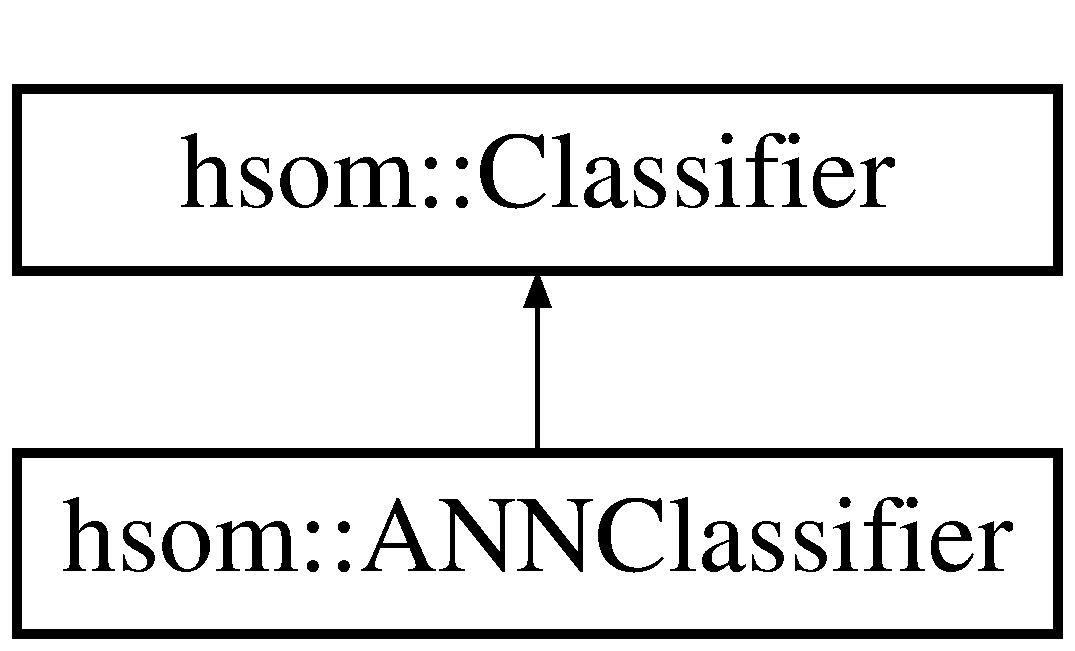
\includegraphics[height=2.000000cm]{classhsom_1_1_a_n_n_classifier}
\end{center}
\end{figure}
\subsection*{\-Public \-Member \-Functions}
\begin{DoxyCompactItemize}
\item 
\hypertarget{classhsom_1_1_a_n_n_classifier_a1af6ffad791c85dd9629131c5c5020f9}{{\bfseries \-A\-N\-N\-Classifier} (\-Q\-String file\-Name)}\label{classhsom_1_1_a_n_n_classifier_a1af6ffad791c85dd9629131c5c5020f9}

\item 
virtual void \hyperlink{classhsom_1_1_a_n_n_classifier_a2777506e21fc1fcb2900ede529aaefac}{classify} (\-Suspect\-Ptr suspect)
\begin{DoxyCompactList}\small\item\em \-Classifies a single suspect. \end{DoxyCompactList}\end{DoxyCompactItemize}
\subsection*{\-Protected \-Member \-Functions}
\begin{DoxyCompactItemize}
\item 
virtual void \hyperlink{classhsom_1_1_a_n_n_classifier_a615dc19a6aa3f45ee00926e2707386e0}{read\-Classifier\-Data} (\-Q\-Dom\-Element \&element)
\begin{DoxyCompactList}\small\item\em \-Interfaces with the \-Persist\-X\-M\-L \-A\-P\-I to ensure correct loading order for a classifier. \end{DoxyCompactList}\item 
virtual void \hyperlink{classhsom_1_1_a_n_n_classifier_a16189d3191b92fefe2f3103b5b789a9d}{write\-Classifier\-Data} (\-Q\-Dom\-Element \&element)
\begin{DoxyCompactList}\small\item\em \-Interfaces with the \-Persist\-X\-M\-L \-A\-P\-I to ensure correct saving order for a classifier. \end{DoxyCompactList}\item 
virtual void \hyperlink{classhsom_1_1_a_n_n_classifier_ac3f43b1ab6681ad13acc52924e3c3fc5}{train\-Classifier} (\-Q\-Vector$<$ \-Suspect\-Ptr $>$ suspects, \-Q\-Map$<$ \-Q\-String, \-Q\-Variant $>$ training\-Parameters)
\begin{DoxyCompactList}\small\item\em \-Performs specific training algorithm for a classifier. \end{DoxyCompactList}\end{DoxyCompactItemize}


\subsection{\-Member \-Function \-Documentation}
\hypertarget{classhsom_1_1_a_n_n_classifier_a2777506e21fc1fcb2900ede529aaefac}{\index{hsom\-::\-A\-N\-N\-Classifier@{hsom\-::\-A\-N\-N\-Classifier}!classify@{classify}}
\index{classify@{classify}!hsom::ANNClassifier@{hsom\-::\-A\-N\-N\-Classifier}}
\subsubsection[{classify}]{\setlength{\rightskip}{0pt plus 5cm}void {\bf hsom\-::\-A\-N\-N\-Classifier\-::classify} (
\begin{DoxyParamCaption}
\item[{\-Suspect\-Ptr}]{suspect}
\end{DoxyParamCaption}
)\hspace{0.3cm}{\ttfamily  \mbox{[}virtual\mbox{]}}}}\label{classhsom_1_1_a_n_n_classifier_a2777506e21fc1fcb2900ede529aaefac}


\-Classifies a single suspect. 

\begin{DoxyRefDesc}{\-Todo}
\item[\hyperlink{todo__todo000003}{\-Todo}]\-Move the input and output width parameters down into the base class \end{DoxyRefDesc}


\begin{DoxyRefDesc}{\-Todo}
\item[\hyperlink{todo__todo000004}{\-Todo}]ensure that the output widths match \end{DoxyRefDesc}


\-Implements \hyperlink{classhsom_1_1_classifier_afe72e6af42ffe1bc2921b3ade481d800}{hsom\-::\-Classifier}.

\hypertarget{classhsom_1_1_a_n_n_classifier_a615dc19a6aa3f45ee00926e2707386e0}{\index{hsom\-::\-A\-N\-N\-Classifier@{hsom\-::\-A\-N\-N\-Classifier}!read\-Classifier\-Data@{read\-Classifier\-Data}}
\index{read\-Classifier\-Data@{read\-Classifier\-Data}!hsom::ANNClassifier@{hsom\-::\-A\-N\-N\-Classifier}}
\subsubsection[{read\-Classifier\-Data}]{\setlength{\rightskip}{0pt plus 5cm}void {\bf hsom\-::\-A\-N\-N\-Classifier\-::read\-Classifier\-Data} (
\begin{DoxyParamCaption}
\item[{\-Q\-Dom\-Element \&}]{element}
\end{DoxyParamCaption}
)\hspace{0.3cm}{\ttfamily  \mbox{[}protected, virtual\mbox{]}}}}\label{classhsom_1_1_a_n_n_classifier_a615dc19a6aa3f45ee00926e2707386e0}


\-Interfaces with the \-Persist\-X\-M\-L \-A\-P\-I to ensure correct loading order for a classifier. 

\begin{DoxyNote}{\-Note}
\-This is optional. \-If not implemented by a derived class, this function does nothing 
\end{DoxyNote}
\begin{DoxyRefDesc}{\-Todo}
\item[\hyperlink{todo__todo000001}{\-Todo}]\-Insert some sort of verification here to make sure that the load went ok \end{DoxyRefDesc}


\-Reimplemented from \hyperlink{classhsom_1_1_classifier_a7005afab0da6cfd49119ba21e31f0d35}{hsom\-::\-Classifier}.

\hypertarget{classhsom_1_1_a_n_n_classifier_ac3f43b1ab6681ad13acc52924e3c3fc5}{\index{hsom\-::\-A\-N\-N\-Classifier@{hsom\-::\-A\-N\-N\-Classifier}!train\-Classifier@{train\-Classifier}}
\index{train\-Classifier@{train\-Classifier}!hsom::ANNClassifier@{hsom\-::\-A\-N\-N\-Classifier}}
\subsubsection[{train\-Classifier}]{\setlength{\rightskip}{0pt plus 5cm}void {\bf hsom\-::\-A\-N\-N\-Classifier\-::train\-Classifier} (
\begin{DoxyParamCaption}
\item[{\-Q\-Vector$<$ \-Suspect\-Ptr $>$}]{suspects, }
\item[{\-Q\-Map$<$ \-Q\-String, \-Q\-Variant $>$}]{training\-Parameters}
\end{DoxyParamCaption}
)\hspace{0.3cm}{\ttfamily  \mbox{[}protected, virtual\mbox{]}}}}\label{classhsom_1_1_a_n_n_classifier_ac3f43b1ab6681ad13acc52924e3c3fc5}


\-Performs specific training algorithm for a classifier. 

\begin{DoxyRefDesc}{\-Todo}
\item[\hyperlink{todo__todo000002}{\-Todo}]\-Move the input and output width parameters down into the base class \end{DoxyRefDesc}


\-Implements \hyperlink{classhsom_1_1_classifier_a1f622d490d89f851c8641b0401648acb}{hsom\-::\-Classifier}.

\hypertarget{classhsom_1_1_a_n_n_classifier_a16189d3191b92fefe2f3103b5b789a9d}{\index{hsom\-::\-A\-N\-N\-Classifier@{hsom\-::\-A\-N\-N\-Classifier}!write\-Classifier\-Data@{write\-Classifier\-Data}}
\index{write\-Classifier\-Data@{write\-Classifier\-Data}!hsom::ANNClassifier@{hsom\-::\-A\-N\-N\-Classifier}}
\subsubsection[{write\-Classifier\-Data}]{\setlength{\rightskip}{0pt plus 5cm}void {\bf hsom\-::\-A\-N\-N\-Classifier\-::write\-Classifier\-Data} (
\begin{DoxyParamCaption}
\item[{\-Q\-Dom\-Element \&}]{element}
\end{DoxyParamCaption}
)\hspace{0.3cm}{\ttfamily  \mbox{[}protected, virtual\mbox{]}}}}\label{classhsom_1_1_a_n_n_classifier_a16189d3191b92fefe2f3103b5b789a9d}


\-Interfaces with the \-Persist\-X\-M\-L \-A\-P\-I to ensure correct saving order for a classifier. 

\begin{DoxyNote}{\-Note}
\-This is optional. \-If not implemented by a derived class, this function does nothing 
\end{DoxyNote}


\-Reimplemented from \hyperlink{classhsom_1_1_classifier_a44fd60ca14d06f5f3889e3d49573cd75}{hsom\-::\-Classifier}.



\-The documentation for this class was generated from the following files\-:\begin{DoxyCompactItemize}
\item 
\-C\-:/\-Users/d3x874/\-Documents/source/urania/classifiers/annclassifier.\-h\item 
\-C\-:/\-Users/d3x874/\-Documents/source/urania/classifiers/annclassifier.\-cpp\end{DoxyCompactItemize}

\hypertarget{classhsom_1_1_classifier}{\section{hsom\-:\-:\-Classifier \-Class \-Reference}
\label{classhsom_1_1_classifier}\index{hsom\-::\-Classifier@{hsom\-::\-Classifier}}
}
\-Inheritance diagram for hsom\-:\-:\-Classifier\-:\begin{figure}[H]
\begin{center}
\leavevmode
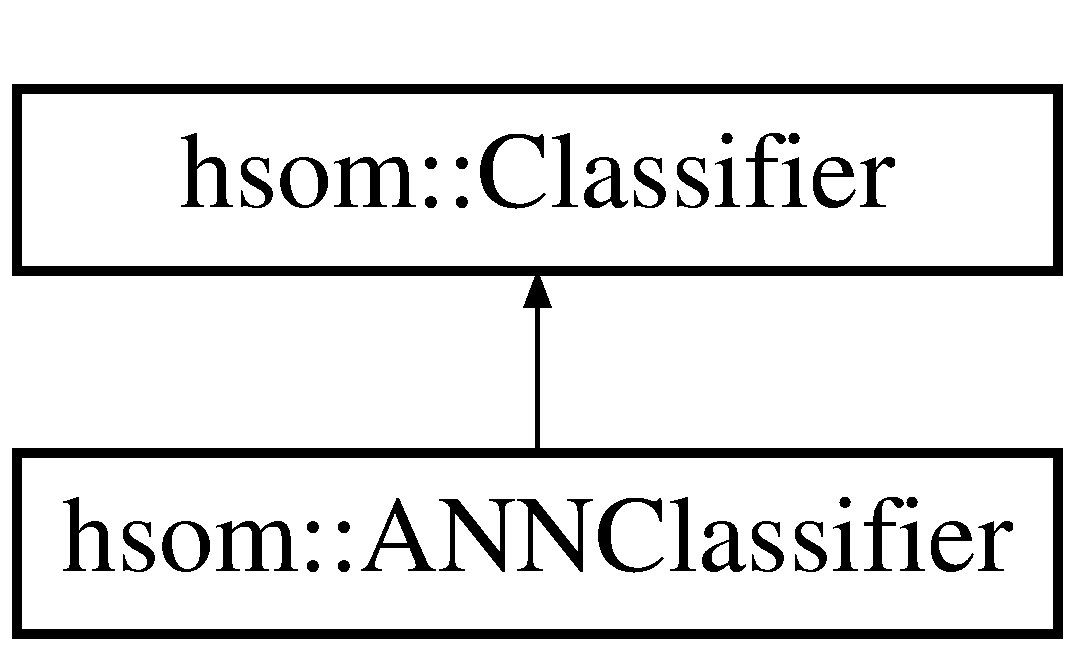
\includegraphics[height=2.000000cm]{classhsom_1_1_classifier}
\end{center}
\end{figure}
\subsection*{\-Public \-Member \-Functions}
\begin{DoxyCompactItemize}
\item 
\hypertarget{classhsom_1_1_classifier_a10514744eb67348a8dd8f71ec2c1631e}{\hyperlink{classhsom_1_1_classifier_a10514744eb67348a8dd8f71ec2c1631e}{\-Classifier} ()}\label{classhsom_1_1_classifier_a10514744eb67348a8dd8f71ec2c1631e}

\begin{DoxyCompactList}\small\item\em \-Constructs a classifier base instance. \end{DoxyCompactList}\item 
void \hyperlink{classhsom_1_1_classifier_a86175b0c10c80d7e0ea84e608ec49d19}{train} (\-Q\-Vector$<$ \-Suspect\-Ptr $>$ suspects, \-Q\-Map$<$ \-Q\-String, \-Q\-Variant $>$ training\-Parameters)
\begin{DoxyCompactList}\small\item\em \-Trains the classifier using a collection of known suspects. \end{DoxyCompactList}\item 
virtual void \hyperlink{classhsom_1_1_classifier_afe72e6af42ffe1bc2921b3ade481d800}{classify} (\-Suspect\-Ptr suspect)=0
\begin{DoxyCompactList}\small\item\em \-Classifies a single suspect. \end{DoxyCompactList}\item 
\hypertarget{classhsom_1_1_classifier_ad7a6005aea99220ef0391b1155310337}{virtual void {\bfseries read\-Data} (\-Q\-Dom\-Element \&element)}\label{classhsom_1_1_classifier_ad7a6005aea99220ef0391b1155310337}

\item 
\hypertarget{classhsom_1_1_classifier_a526942872ee1edea3ac51e37f0f45231}{virtual void {\bfseries write\-Data} (\-Q\-Dom\-Element \&element)}\label{classhsom_1_1_classifier_a526942872ee1edea3ac51e37f0f45231}

\end{DoxyCompactItemize}
\subsection*{\-Protected \-Member \-Functions}
\begin{DoxyCompactItemize}
\item 
virtual void \hyperlink{classhsom_1_1_classifier_a7005afab0da6cfd49119ba21e31f0d35}{read\-Classifier\-Data} (\-Q\-Dom\-Element \&element)
\begin{DoxyCompactList}\small\item\em \-Interfaces with the \-Persist\-X\-M\-L \-A\-P\-I to ensure correct loading order for a classifier. \end{DoxyCompactList}\item 
virtual void \hyperlink{classhsom_1_1_classifier_a44fd60ca14d06f5f3889e3d49573cd75}{write\-Classifier\-Data} (\-Q\-Dom\-Element \&element)
\begin{DoxyCompactList}\small\item\em \-Interfaces with the \-Persist\-X\-M\-L \-A\-P\-I to ensure correct saving order for a classifier. \end{DoxyCompactList}\item 
virtual void \hyperlink{classhsom_1_1_classifier_a1f622d490d89f851c8641b0401648acb}{train\-Classifier} (\-Q\-Vector$<$ \-Suspect\-Ptr $>$ suspects, \-Q\-Map$<$ \-Q\-String, \-Q\-Variant $>$ training\-Parameters)=0
\begin{DoxyCompactList}\small\item\em \-Performs specific training algorithm for a classifier. \end{DoxyCompactList}\end{DoxyCompactItemize}
\subsection*{\-Protected \-Attributes}
\begin{DoxyCompactItemize}
\item 
\hypertarget{classhsom_1_1_classifier_a57f42894e3369a20b4fd0f3dd8f3d8a5}{\-Q\-Map$<$ \-Q\-String, \-Q\-Variant $>$ \hyperlink{classhsom_1_1_classifier_a57f42894e3369a20b4fd0f3dd8f3d8a5}{\-\_\-training\-Parameters}}\label{classhsom_1_1_classifier_a57f42894e3369a20b4fd0f3dd8f3d8a5}

\begin{DoxyCompactList}\small\item\em \-Describes the parameters used to tune the training of this classifier. \end{DoxyCompactList}\end{DoxyCompactItemize}


\subsection{\-Member \-Function \-Documentation}
\hypertarget{classhsom_1_1_classifier_afe72e6af42ffe1bc2921b3ade481d800}{\index{hsom\-::\-Classifier@{hsom\-::\-Classifier}!classify@{classify}}
\index{classify@{classify}!hsom::Classifier@{hsom\-::\-Classifier}}
\subsubsection[{classify}]{\setlength{\rightskip}{0pt plus 5cm}virtual void {\bf hsom\-::\-Classifier\-::classify} (
\begin{DoxyParamCaption}
\item[{\-Suspect\-Ptr}]{suspect}
\end{DoxyParamCaption}
)\hspace{0.3cm}{\ttfamily  \mbox{[}pure virtual\mbox{]}}}}\label{classhsom_1_1_classifier_afe72e6af42ffe1bc2921b3ade481d800}


\-Classifies a single suspect. 


\begin{DoxyParams}{\-Parameters}
{\em suspect} & \-The suspect to be classified \\
\hline
\end{DoxyParams}


\-Implemented in \hyperlink{classhsom_1_1_a_n_n_classifier_a2777506e21fc1fcb2900ede529aaefac}{hsom\-::\-A\-N\-N\-Classifier}.

\hypertarget{classhsom_1_1_classifier_a7005afab0da6cfd49119ba21e31f0d35}{\index{hsom\-::\-Classifier@{hsom\-::\-Classifier}!read\-Classifier\-Data@{read\-Classifier\-Data}}
\index{read\-Classifier\-Data@{read\-Classifier\-Data}!hsom::Classifier@{hsom\-::\-Classifier}}
\subsubsection[{read\-Classifier\-Data}]{\setlength{\rightskip}{0pt plus 5cm}void {\bf hsom\-::\-Classifier\-::read\-Classifier\-Data} (
\begin{DoxyParamCaption}
\item[{\-Q\-Dom\-Element \&}]{element}
\end{DoxyParamCaption}
)\hspace{0.3cm}{\ttfamily  \mbox{[}protected, virtual\mbox{]}}}}\label{classhsom_1_1_classifier_a7005afab0da6cfd49119ba21e31f0d35}


\-Interfaces with the \-Persist\-X\-M\-L \-A\-P\-I to ensure correct loading order for a classifier. 

\begin{DoxyNote}{\-Note}
\-This is optional. \-If not implemented by a derived class, this function does nothing 
\end{DoxyNote}


\-Reimplemented in \hyperlink{classhsom_1_1_a_n_n_classifier_a615dc19a6aa3f45ee00926e2707386e0}{hsom\-::\-A\-N\-N\-Classifier}.

\hypertarget{classhsom_1_1_classifier_a86175b0c10c80d7e0ea84e608ec49d19}{\index{hsom\-::\-Classifier@{hsom\-::\-Classifier}!train@{train}}
\index{train@{train}!hsom::Classifier@{hsom\-::\-Classifier}}
\subsubsection[{train}]{\setlength{\rightskip}{0pt plus 5cm}void {\bf hsom\-::\-Classifier\-::train} (
\begin{DoxyParamCaption}
\item[{\-Q\-Vector$<$ \-Suspect\-Ptr $>$}]{suspects, }
\item[{\-Q\-Map$<$ \-Q\-String, \-Q\-Variant $>$}]{training\-Parameters}
\end{DoxyParamCaption}
)}}\label{classhsom_1_1_classifier_a86175b0c10c80d7e0ea84e608ec49d19}


\-Trains the classifier using a collection of known suspects. 


\begin{DoxyParams}{\-Parameters}
{\em suspects} & \-The list of suspects with which to train this classifier \\
\hline
{\em training\-Parameters} & \-The tuning parameters used to train this classifier \\
\hline
\end{DoxyParams}
\hypertarget{classhsom_1_1_classifier_a1f622d490d89f851c8641b0401648acb}{\index{hsom\-::\-Classifier@{hsom\-::\-Classifier}!train\-Classifier@{train\-Classifier}}
\index{train\-Classifier@{train\-Classifier}!hsom::Classifier@{hsom\-::\-Classifier}}
\subsubsection[{train\-Classifier}]{\setlength{\rightskip}{0pt plus 5cm}virtual void {\bf hsom\-::\-Classifier\-::train\-Classifier} (
\begin{DoxyParamCaption}
\item[{\-Q\-Vector$<$ \-Suspect\-Ptr $>$}]{suspects, }
\item[{\-Q\-Map$<$ \-Q\-String, \-Q\-Variant $>$}]{training\-Parameters}
\end{DoxyParamCaption}
)\hspace{0.3cm}{\ttfamily  \mbox{[}protected, pure virtual\mbox{]}}}}\label{classhsom_1_1_classifier_a1f622d490d89f851c8641b0401648acb}


\-Performs specific training algorithm for a classifier. 


\begin{DoxyParams}{\-Parameters}
{\em suspects} & \-The list of suspects with which to train this classifier \\
\hline
{\em training\-Parameters} & \-The tuning parameters used to train this classifier \\
\hline
\end{DoxyParams}


\-Implemented in \hyperlink{classhsom_1_1_a_n_n_classifier_ac3f43b1ab6681ad13acc52924e3c3fc5}{hsom\-::\-A\-N\-N\-Classifier}.

\hypertarget{classhsom_1_1_classifier_a44fd60ca14d06f5f3889e3d49573cd75}{\index{hsom\-::\-Classifier@{hsom\-::\-Classifier}!write\-Classifier\-Data@{write\-Classifier\-Data}}
\index{write\-Classifier\-Data@{write\-Classifier\-Data}!hsom::Classifier@{hsom\-::\-Classifier}}
\subsubsection[{write\-Classifier\-Data}]{\setlength{\rightskip}{0pt plus 5cm}void {\bf hsom\-::\-Classifier\-::write\-Classifier\-Data} (
\begin{DoxyParamCaption}
\item[{\-Q\-Dom\-Element \&}]{element}
\end{DoxyParamCaption}
)\hspace{0.3cm}{\ttfamily  \mbox{[}protected, virtual\mbox{]}}}}\label{classhsom_1_1_classifier_a44fd60ca14d06f5f3889e3d49573cd75}


\-Interfaces with the \-Persist\-X\-M\-L \-A\-P\-I to ensure correct saving order for a classifier. 

\begin{DoxyNote}{\-Note}
\-This is optional. \-If not implemented by a derived class, this function does nothing 
\end{DoxyNote}


\-Reimplemented in \hyperlink{classhsom_1_1_a_n_n_classifier_a16189d3191b92fefe2f3103b5b789a9d}{hsom\-::\-A\-N\-N\-Classifier}.



\-The documentation for this class was generated from the following files\-:\begin{DoxyCompactItemize}
\item 
\-C\-:/\-Users/d3x874/\-Documents/source/urania/classifiers/classifier.\-h\item 
\-C\-:/\-Users/d3x874/\-Documents/source/urania/classifiers/classifier.\-cpp\end{DoxyCompactItemize}

\hypertarget{class_color_feature}{\section{\-Color\-Feature \-Class \-Reference}
\label{class_color_feature}\index{\-Color\-Feature@{\-Color\-Feature}}
}
\subsection*{\-Public \-Member \-Functions}
\begin{DoxyCompactItemize}
\item 
\hypertarget{class_color_feature_a92a4e970e61c6222a748790456a1142f}{{\bfseries \-Color\-Feature} (double red, double green, double blue)}\label{class_color_feature_a92a4e970e61c6222a748790456a1142f}

\end{DoxyCompactItemize}


\-The documentation for this class was generated from the following files\-:\begin{DoxyCompactItemize}
\item 
\-C\-:/\-Users/d3x874/\-Documents/source/urania/colorfeature.\-h\item 
\-C\-:/\-Users/d3x874/\-Documents/source/urania/colorfeature.\-cpp\end{DoxyCompactItemize}

\hypertarget{class_color_suspect}{\section{\-Color\-Suspect \-Class \-Reference}
\label{class_color_suspect}\index{\-Color\-Suspect@{\-Color\-Suspect}}
}
\subsection*{\-Public \-Member \-Functions}
\begin{DoxyCompactItemize}
\item 
\hyperlink{class_color_suspect_afbbbbd9c577ff42ecada23b497a451cb}{\-Color\-Suspect} (const cv\-::\-Mat \&img, int real\-Cat, int cat\-Ct, const \-Size\-Plus$<$ int $>$ \&hist\-Sz, std\-::string name)
\item 
virtual \hyperlink{class_color_suspect_acd02132c6855e7a8f63ddd8b5d790996}{$\sim$\-Color\-Suspect} ()
\item 
virtual \-Feature $\ast$ \hyperlink{class_color_suspect_ae9d514be897435ac42d73a7aed5bf855}{get\-Next\-Feature} ()
\end{DoxyCompactItemize}


\subsection{\-Constructor \& \-Destructor \-Documentation}
\hypertarget{class_color_suspect_afbbbbd9c577ff42ecada23b497a451cb}{\index{\-Color\-Suspect@{\-Color\-Suspect}!\-Color\-Suspect@{\-Color\-Suspect}}
\index{\-Color\-Suspect@{\-Color\-Suspect}!ColorSuspect@{\-Color\-Suspect}}
\subsubsection[{\-Color\-Suspect}]{\setlength{\rightskip}{0pt plus 5cm}\-Color\-Suspect\-::\-Color\-Suspect (
\begin{DoxyParamCaption}
\item[{const cv\-::\-Mat \&}]{img, }
\item[{int}]{real\-Cat, }
\item[{int}]{cat\-Ct, }
\item[{const \-Size\-Plus$<$ int $>$ \&}]{hist\-Sz, }
\item[{std\-::string}]{name}
\end{DoxyParamCaption}
)}}\label{class_color_suspect_afbbbbd9c577ff42ecada23b497a451cb}
\-Creates a new \hyperlink{class_color_suspect}{\-Color\-Suspect} 
\begin{DoxyParams}{\-Parameters}
{\em img} & -\/ \-The image that this \-Suspect represents \\
\hline
{\em real\-Cat} & -\/ \-The actual category for this \-Suspect \\
\hline
{\em cat\-Ct} & -\/ \-The number of categories possilbel for this \-Suspect \\
\hline
{\em grid\-Sz} & -\/ \-The size of this \-Suspect's histogram \\
\hline
{\em name} & -\/ \-The name of this \-Suspect \\
\hline
\end{DoxyParams}
\hypertarget{class_color_suspect_acd02132c6855e7a8f63ddd8b5d790996}{\index{\-Color\-Suspect@{\-Color\-Suspect}!$\sim$\-Color\-Suspect@{$\sim$\-Color\-Suspect}}
\index{$\sim$\-Color\-Suspect@{$\sim$\-Color\-Suspect}!ColorSuspect@{\-Color\-Suspect}}
\subsubsection[{$\sim$\-Color\-Suspect}]{\setlength{\rightskip}{0pt plus 5cm}{\bf \-Color\-Suspect\-::$\sim$\-Color\-Suspect} (
\begin{DoxyParamCaption}
{}
\end{DoxyParamCaption}
)\hspace{0.3cm}{\ttfamily  \mbox{[}virtual\mbox{]}}}}\label{class_color_suspect_acd02132c6855e7a8f63ddd8b5d790996}
\-Destructs this suspect 

\subsection{\-Member \-Function \-Documentation}
\hypertarget{class_color_suspect_ae9d514be897435ac42d73a7aed5bf855}{\index{\-Color\-Suspect@{\-Color\-Suspect}!get\-Next\-Feature@{get\-Next\-Feature}}
\index{get\-Next\-Feature@{get\-Next\-Feature}!ColorSuspect@{\-Color\-Suspect}}
\subsubsection[{get\-Next\-Feature}]{\setlength{\rightskip}{0pt plus 5cm}\-Feature $\ast$ {\bf \-Color\-Suspect\-::get\-Next\-Feature} (
\begin{DoxyParamCaption}
{}
\end{DoxyParamCaption}
)\hspace{0.3cm}{\ttfamily  \mbox{[}virtual\mbox{]}}}}\label{class_color_suspect_ae9d514be897435ac42d73a7aed5bf855}
\-Generates the next feature from this \-Suspect 

\-The documentation for this class was generated from the following files\-:\begin{DoxyCompactItemize}
\item 
\-C\-:/\-Users/d3x874/\-Documents/source/urania/suspects/colorsuspect.\-h\item 
\-C\-:/\-Users/d3x874/\-Documents/source/urania/suspects/colorsuspect.\-cpp\end{DoxyCompactItemize}

\hypertarget{classhsom_1_1_fast_hex_grid}{\section{hsom\-:\-:\-Fast\-Hex\-Grid$<$ \-T $>$ \-Class \-Template \-Reference}
\label{classhsom_1_1_fast_hex_grid}\index{hsom\-::\-Fast\-Hex\-Grid$<$ T $>$@{hsom\-::\-Fast\-Hex\-Grid$<$ T $>$}}
}


{\ttfamily \#include $<$fasthexgrid.\-hpp$>$}

\-Inheritance diagram for hsom\-:\-:\-Fast\-Hex\-Grid$<$ \-T $>$\-:\begin{figure}[H]
\begin{center}
\leavevmode
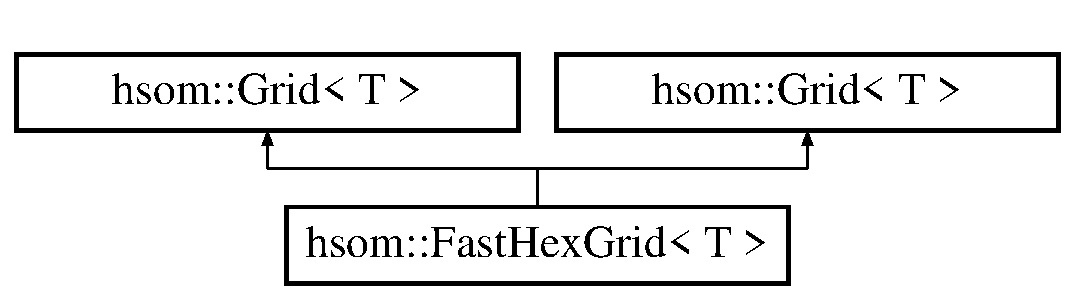
\includegraphics[height=2.000000cm]{classhsom_1_1_fast_hex_grid}
\end{center}
\end{figure}
\subsection*{\-Public \-Member \-Functions}
\begin{DoxyCompactItemize}
\item 
\hypertarget{classhsom_1_1_fast_hex_grid_a7d82cd1ac4c97eac37fd7bf0579d16a3}{\hyperlink{classhsom_1_1_fast_hex_grid_a7d82cd1ac4c97eac37fd7bf0579d16a3}{\-Fast\-Hex\-Grid} ()}\label{classhsom_1_1_fast_hex_grid_a7d82cd1ac4c97eac37fd7bf0579d16a3}

\begin{DoxyCompactList}\small\item\em \-Constructs a hex grid with no size information. \end{DoxyCompactList}\item 
\hyperlink{classhsom_1_1_fast_hex_grid_aec7541c31bf2b26837cdbf887d66fa5a}{\-Fast\-Hex\-Grid} (\-Q\-Vector$<$ int $>$ \hyperlink{classhsom_1_1_grid_a3e846473299eb2c7c259659eb61a6234}{size})
\begin{DoxyCompactList}\small\item\em \-Constructs the hex grid with a specified size. \end{DoxyCompactList}\item 
\hyperlink{classhsom_1_1_fast_hex_grid_a09b2f049297965971e33ea7d6e583da3}{\-Fast\-Hex\-Grid} (int s)
\begin{DoxyCompactList}\small\item\em \-Constructs the hex grid with a specified size. \end{DoxyCompactList}\item 
\hyperlink{classhsom_1_1_fast_hex_grid_a9dc41236780c5544948dfe3dd5cccf3e}{\-Fast\-Hex\-Grid} (\-Q\-Vector$<$ int $>$ \hyperlink{classhsom_1_1_grid_a3e846473299eb2c7c259659eb61a6234}{size}, \-Q\-Vector$<$ \-T $>$ \hyperlink{classhsom_1_1_grid_ae6b6ffb72e86c3904e8ac21253d85a24}{items})
\begin{DoxyCompactList}\small\item\em \-Constructs the hex grid with the specified size and fills it with the supplied values. \end{DoxyCompactList}\item 
\hyperlink{classhsom_1_1_fast_hex_grid_ad8e600cd2711e0882b3a97a3facbca8e}{\-Fast\-Hex\-Grid} (int s, \-Q\-Vector$<$ \-T $>$ \hyperlink{classhsom_1_1_grid_ae6b6ffb72e86c3904e8ac21253d85a24}{items})
\begin{DoxyCompactList}\small\item\em \-Constructs the hex grid with the specified size and fills it with the supplied values. \end{DoxyCompactList}\item 
\hypertarget{classhsom_1_1_fast_hex_grid_a9afacd0fd3f937ff69f14b196bef9cfa}{virtual \hyperlink{classhsom_1_1_fast_hex_grid_a9afacd0fd3f937ff69f14b196bef9cfa}{$\sim$\-Fast\-Hex\-Grid} ()}\label{classhsom_1_1_fast_hex_grid_a9afacd0fd3f937ff69f14b196bef9cfa}

\begin{DoxyCompactList}\small\item\em \-Destructs the \hyperlink{classhsom_1_1_hex_grid}{\-Hex\-Grid}. \end{DoxyCompactList}\item 
\hypertarget{classhsom_1_1_fast_hex_grid_a262cbfb75a0861ac88d5d79112e157a7}{int {\bfseries s} ()}\label{classhsom_1_1_fast_hex_grid_a262cbfb75a0861ac88d5d79112e157a7}

\item 
\hypertarget{classhsom_1_1_fast_hex_grid_a2e66b85ee6f69bc1fa7cd51cec4dcd2e}{virtual void \hyperlink{classhsom_1_1_fast_hex_grid_a2e66b85ee6f69bc1fa7cd51cec4dcd2e}{check\-Size} (\-Q\-Vector$<$ int $>$ \hyperlink{classhsom_1_1_grid_a3e846473299eb2c7c259659eb61a6234}{size})}\label{classhsom_1_1_fast_hex_grid_a2e66b85ee6f69bc1fa7cd51cec4dcd2e}

\begin{DoxyCompactList}\small\item\em \-Checks the supplied size to ensure that it is valid for the \hyperlink{classhsom_1_1_grid}{\-Grid}. \end{DoxyCompactList}\item 
\hypertarget{classhsom_1_1_fast_hex_grid_a592489c96e73a494258e46e02e324eec}{virtual int \hyperlink{classhsom_1_1_fast_hex_grid_a592489c96e73a494258e46e02e324eec}{capacity\-From\-Size} (\-Q\-Vector$<$ int $>$ \hyperlink{classhsom_1_1_grid_a3e846473299eb2c7c259659eb61a6234}{size})}\label{classhsom_1_1_fast_hex_grid_a592489c96e73a494258e46e02e324eec}

\begin{DoxyCompactList}\small\item\em \-Gets the capacity of a grid based on the size of the grid. \end{DoxyCompactList}\item 
\hypertarget{classhsom_1_1_fast_hex_grid_a8617bee85643b77b31b54644f019ceb3}{virtual void \hyperlink{classhsom_1_1_fast_hex_grid_a8617bee85643b77b31b54644f019ceb3}{check\-Coords} (\-Q\-Vector$<$ int $>$ \hyperlink{classhsom_1_1_fast_hex_grid_a5305b83a2932122381f5c78a162cd147}{coords})}\label{classhsom_1_1_fast_hex_grid_a8617bee85643b77b31b54644f019ceb3}

\begin{DoxyCompactList}\small\item\em \-Checks a given point to ensure it is a valid reference to an element in the grid. \end{DoxyCompactList}\item 
virtual int \hyperlink{classhsom_1_1_fast_hex_grid_a74ef97079e75235a07f9dc70bdbf238a}{index} (\-Q\-Vector$<$ int $>$ \hyperlink{classhsom_1_1_fast_hex_grid_a5305b83a2932122381f5c78a162cd147}{coords})
\begin{DoxyCompactList}\small\item\em \-Fetches the index for the slot at the specified coordinates. \end{DoxyCompactList}\item 
virtual \-Q\-Vector$<$ int $>$ \hyperlink{classhsom_1_1_fast_hex_grid_a5305b83a2932122381f5c78a162cd147}{coords} (int idx)
\begin{DoxyCompactList}\small\item\em \-Fetches the coordinates given an index. \end{DoxyCompactList}\item 
\hypertarget{classhsom_1_1_fast_hex_grid_aaae85f5b93f54a9e8100f4b3335708d8}{virtual \-Q\-Vector$<$ double $>$ \hyperlink{classhsom_1_1_fast_hex_grid_aaae85f5b93f54a9e8100f4b3335708d8}{real\-Bounds} ()}\label{classhsom_1_1_fast_hex_grid_aaae85f5b93f54a9e8100f4b3335708d8}

\begin{DoxyCompactList}\small\item\em \-Fetches the extents of the real coordinate mapping space ( should only be used for visualization ) \end{DoxyCompactList}\item 
\hypertarget{classhsom_1_1_fast_hex_grid_a3c8c27adc0c2bc408b45d831997f2799}{virtual \-Q\-Vector$<$ double $>$ \hyperlink{classhsom_1_1_fast_hex_grid_a3c8c27adc0c2bc408b45d831997f2799}{real\-Coords} (int idx)}\label{classhsom_1_1_fast_hex_grid_a3c8c27adc0c2bc408b45d831997f2799}

\begin{DoxyCompactList}\small\item\em \-Fetches the real coordinates of a given index in the grid ( should only be used for visualization ) \end{DoxyCompactList}\item 
virtual int \hyperlink{classhsom_1_1_fast_hex_grid_a7fc65f0095eb0b5e14d41b116ea140d4}{diagonal} ()
\begin{DoxyCompactList}\small\item\em \-Fetches the length of the major diagonal running through the grid. \end{DoxyCompactList}\item 
\hypertarget{classhsom_1_1_fast_hex_grid_a5577744b71fe38a5825e56a80f470c68}{virtual int \hyperlink{classhsom_1_1_fast_hex_grid_a5577744b71fe38a5825e56a80f470c68}{distance} (int idx0, int idx1)}\label{classhsom_1_1_fast_hex_grid_a5577744b71fe38a5825e56a80f470c68}

\begin{DoxyCompactList}\small\item\em \-Fetches the distance between two cells in the grid. \end{DoxyCompactList}\item 
\hypertarget{classhsom_1_1_fast_hex_grid_a7d82cd1ac4c97eac37fd7bf0579d16a3}{\hyperlink{classhsom_1_1_fast_hex_grid_a7d82cd1ac4c97eac37fd7bf0579d16a3}{\-Fast\-Hex\-Grid} ()}\label{classhsom_1_1_fast_hex_grid_a7d82cd1ac4c97eac37fd7bf0579d16a3}

\begin{DoxyCompactList}\small\item\em \-Constructs a hex grid with no size information. \end{DoxyCompactList}\item 
\hyperlink{classhsom_1_1_fast_hex_grid_aec7541c31bf2b26837cdbf887d66fa5a}{\-Fast\-Hex\-Grid} (\-Q\-Vector$<$ int $>$ \hyperlink{classhsom_1_1_grid_a3e846473299eb2c7c259659eb61a6234}{size})
\begin{DoxyCompactList}\small\item\em \-Constructs the hex grid with a specified size. \end{DoxyCompactList}\item 
\hyperlink{classhsom_1_1_fast_hex_grid_a09b2f049297965971e33ea7d6e583da3}{\-Fast\-Hex\-Grid} (int s)
\begin{DoxyCompactList}\small\item\em \-Constructs the hex grid with a specified size. \end{DoxyCompactList}\item 
\hyperlink{classhsom_1_1_fast_hex_grid_a9dc41236780c5544948dfe3dd5cccf3e}{\-Fast\-Hex\-Grid} (\-Q\-Vector$<$ int $>$ \hyperlink{classhsom_1_1_grid_a3e846473299eb2c7c259659eb61a6234}{size}, \-Q\-Vector$<$ \-T $>$ \hyperlink{classhsom_1_1_grid_ae6b6ffb72e86c3904e8ac21253d85a24}{items})
\begin{DoxyCompactList}\small\item\em \-Constructs the hex grid with the specified size and fills it with the supplied values. \end{DoxyCompactList}\item 
\hyperlink{classhsom_1_1_fast_hex_grid_ad8e600cd2711e0882b3a97a3facbca8e}{\-Fast\-Hex\-Grid} (int s, \-Q\-Vector$<$ \-T $>$ \hyperlink{classhsom_1_1_grid_ae6b6ffb72e86c3904e8ac21253d85a24}{items})
\begin{DoxyCompactList}\small\item\em \-Constructs the hex grid with the specified size and fills it with the supplied values. \end{DoxyCompactList}\item 
\hypertarget{classhsom_1_1_fast_hex_grid_a9afacd0fd3f937ff69f14b196bef9cfa}{virtual \hyperlink{classhsom_1_1_fast_hex_grid_a9afacd0fd3f937ff69f14b196bef9cfa}{$\sim$\-Fast\-Hex\-Grid} ()}\label{classhsom_1_1_fast_hex_grid_a9afacd0fd3f937ff69f14b196bef9cfa}

\begin{DoxyCompactList}\small\item\em \-Destructs the \hyperlink{classhsom_1_1_hex_grid}{\-Hex\-Grid}. \end{DoxyCompactList}\item 
\hypertarget{classhsom_1_1_fast_hex_grid_a262cbfb75a0861ac88d5d79112e157a7}{int {\bfseries s} ()}\label{classhsom_1_1_fast_hex_grid_a262cbfb75a0861ac88d5d79112e157a7}

\item 
\hypertarget{classhsom_1_1_fast_hex_grid_a2e66b85ee6f69bc1fa7cd51cec4dcd2e}{virtual void \hyperlink{classhsom_1_1_fast_hex_grid_a2e66b85ee6f69bc1fa7cd51cec4dcd2e}{check\-Size} (\-Q\-Vector$<$ int $>$ \hyperlink{classhsom_1_1_grid_a3e846473299eb2c7c259659eb61a6234}{size})}\label{classhsom_1_1_fast_hex_grid_a2e66b85ee6f69bc1fa7cd51cec4dcd2e}

\begin{DoxyCompactList}\small\item\em \-Checks the supplied size to ensure that it is valid for the \hyperlink{classhsom_1_1_grid}{\-Grid}. \end{DoxyCompactList}\item 
\hypertarget{classhsom_1_1_fast_hex_grid_a592489c96e73a494258e46e02e324eec}{virtual int \hyperlink{classhsom_1_1_fast_hex_grid_a592489c96e73a494258e46e02e324eec}{capacity\-From\-Size} (\-Q\-Vector$<$ int $>$ \hyperlink{classhsom_1_1_grid_a3e846473299eb2c7c259659eb61a6234}{size})}\label{classhsom_1_1_fast_hex_grid_a592489c96e73a494258e46e02e324eec}

\begin{DoxyCompactList}\small\item\em \-Gets the capacity of a grid based on the size of the grid. \end{DoxyCompactList}\item 
\hypertarget{classhsom_1_1_fast_hex_grid_a8617bee85643b77b31b54644f019ceb3}{virtual void \hyperlink{classhsom_1_1_fast_hex_grid_a8617bee85643b77b31b54644f019ceb3}{check\-Coords} (\-Q\-Vector$<$ int $>$ \hyperlink{classhsom_1_1_fast_hex_grid_a5305b83a2932122381f5c78a162cd147}{coords})}\label{classhsom_1_1_fast_hex_grid_a8617bee85643b77b31b54644f019ceb3}

\begin{DoxyCompactList}\small\item\em \-Checks a given point to ensure it is a valid reference to an element in the grid. \end{DoxyCompactList}\item 
virtual int \hyperlink{classhsom_1_1_fast_hex_grid_a74ef97079e75235a07f9dc70bdbf238a}{index} (\-Q\-Vector$<$ int $>$ \hyperlink{classhsom_1_1_fast_hex_grid_a5305b83a2932122381f5c78a162cd147}{coords})
\begin{DoxyCompactList}\small\item\em \-Fetches the index for the slot at the specified coordinates. \end{DoxyCompactList}\item 
virtual \-Q\-Vector$<$ int $>$ \hyperlink{classhsom_1_1_fast_hex_grid_a5305b83a2932122381f5c78a162cd147}{coords} (int idx)
\begin{DoxyCompactList}\small\item\em \-Fetches the coordinates given an index. \end{DoxyCompactList}\item 
\hypertarget{classhsom_1_1_fast_hex_grid_aaae85f5b93f54a9e8100f4b3335708d8}{virtual \-Q\-Vector$<$ double $>$ \hyperlink{classhsom_1_1_fast_hex_grid_aaae85f5b93f54a9e8100f4b3335708d8}{real\-Bounds} ()}\label{classhsom_1_1_fast_hex_grid_aaae85f5b93f54a9e8100f4b3335708d8}

\begin{DoxyCompactList}\small\item\em \-Fetches the extents of the real coordinate mapping space ( should only be used for visualization ) \end{DoxyCompactList}\item 
\hypertarget{classhsom_1_1_fast_hex_grid_a3c8c27adc0c2bc408b45d831997f2799}{virtual \-Q\-Vector$<$ double $>$ \hyperlink{classhsom_1_1_fast_hex_grid_a3c8c27adc0c2bc408b45d831997f2799}{real\-Coords} (int idx)}\label{classhsom_1_1_fast_hex_grid_a3c8c27adc0c2bc408b45d831997f2799}

\begin{DoxyCompactList}\small\item\em \-Fetches the real coordinates of a given index in the grid ( should only be used for visualization ) \end{DoxyCompactList}\item 
virtual int \hyperlink{classhsom_1_1_fast_hex_grid_a7fc65f0095eb0b5e14d41b116ea140d4}{diagonal} ()
\begin{DoxyCompactList}\small\item\em \-Fetches the length of the major diagonal running through the grid. \end{DoxyCompactList}\item 
\hypertarget{classhsom_1_1_fast_hex_grid_a5577744b71fe38a5825e56a80f470c68}{virtual int \hyperlink{classhsom_1_1_fast_hex_grid_a5577744b71fe38a5825e56a80f470c68}{distance} (int idx0, int idx1)}\label{classhsom_1_1_fast_hex_grid_a5577744b71fe38a5825e56a80f470c68}

\begin{DoxyCompactList}\small\item\em \-Fetches the distance between two cells in the grid. \end{DoxyCompactList}\end{DoxyCompactItemize}


\subsection{\-Detailed \-Description}
\subsubsection*{template$<$class T$>$class hsom\-::\-Fast\-Hex\-Grid$<$ T $>$}

\-The \hyperlink{classhsom_1_1_hex_grid}{\-Hex\-Grid} class provides the basis for the spatial organization of the \-Self \-Organizing \-Map. \-It provides a hexagonal grid which supports neighborhood searches, edge wrapping, and other functionality. 

\subsection{\-Constructor \& \-Destructor \-Documentation}
\hypertarget{classhsom_1_1_fast_hex_grid_aec7541c31bf2b26837cdbf887d66fa5a}{\index{hsom\-::\-Fast\-Hex\-Grid@{hsom\-::\-Fast\-Hex\-Grid}!\-Fast\-Hex\-Grid@{\-Fast\-Hex\-Grid}}
\index{\-Fast\-Hex\-Grid@{\-Fast\-Hex\-Grid}!hsom::FastHexGrid@{hsom\-::\-Fast\-Hex\-Grid}}
\subsubsection[{\-Fast\-Hex\-Grid}]{\setlength{\rightskip}{0pt plus 5cm}template$<$class T $>$ {\bf hsom\-::\-Fast\-Hex\-Grid}$<$ \-T $>$\-::{\bf \-Fast\-Hex\-Grid} (
\begin{DoxyParamCaption}
\item[{\-Q\-Vector$<$ int $>$}]{size}
\end{DoxyParamCaption}
)\hspace{0.3cm}{\ttfamily  \mbox{[}inline\mbox{]}}}}\label{classhsom_1_1_fast_hex_grid_aec7541c31bf2b26837cdbf887d66fa5a}


\-Constructs the hex grid with a specified size. 


\begin{DoxyParams}{\-Parameters}
{\em size} & \-The size of the new grid \\
\hline
\end{DoxyParams}
\hypertarget{classhsom_1_1_fast_hex_grid_a09b2f049297965971e33ea7d6e583da3}{\index{hsom\-::\-Fast\-Hex\-Grid@{hsom\-::\-Fast\-Hex\-Grid}!\-Fast\-Hex\-Grid@{\-Fast\-Hex\-Grid}}
\index{\-Fast\-Hex\-Grid@{\-Fast\-Hex\-Grid}!hsom::FastHexGrid@{hsom\-::\-Fast\-Hex\-Grid}}
\subsubsection[{\-Fast\-Hex\-Grid}]{\setlength{\rightskip}{0pt plus 5cm}template$<$class T $>$ {\bf hsom\-::\-Fast\-Hex\-Grid}$<$ \-T $>$\-::{\bf \-Fast\-Hex\-Grid} (
\begin{DoxyParamCaption}
\item[{int}]{s}
\end{DoxyParamCaption}
)\hspace{0.3cm}{\ttfamily  \mbox{[}inline\mbox{]}}}}\label{classhsom_1_1_fast_hex_grid_a09b2f049297965971e33ea7d6e583da3}


\-Constructs the hex grid with a specified size. 


\begin{DoxyParams}{\-Parameters}
{\em s} & \-The length of one side of the grid \\
\hline
\end{DoxyParams}
\hypertarget{classhsom_1_1_fast_hex_grid_a9dc41236780c5544948dfe3dd5cccf3e}{\index{hsom\-::\-Fast\-Hex\-Grid@{hsom\-::\-Fast\-Hex\-Grid}!\-Fast\-Hex\-Grid@{\-Fast\-Hex\-Grid}}
\index{\-Fast\-Hex\-Grid@{\-Fast\-Hex\-Grid}!hsom::FastHexGrid@{hsom\-::\-Fast\-Hex\-Grid}}
\subsubsection[{\-Fast\-Hex\-Grid}]{\setlength{\rightskip}{0pt plus 5cm}template$<$class T $>$ {\bf hsom\-::\-Fast\-Hex\-Grid}$<$ \-T $>$\-::{\bf \-Fast\-Hex\-Grid} (
\begin{DoxyParamCaption}
\item[{\-Q\-Vector$<$ int $>$}]{size, }
\item[{\-Q\-Vector$<$ \-T $>$}]{items}
\end{DoxyParamCaption}
)\hspace{0.3cm}{\ttfamily  \mbox{[}inline\mbox{]}}}}\label{classhsom_1_1_fast_hex_grid_a9dc41236780c5544948dfe3dd5cccf3e}


\-Constructs the hex grid with the specified size and fills it with the supplied values. 


\begin{DoxyParams}{\-Parameters}
{\em size} & \-The size of the new grid \\
\hline
{\em items} & \-The items with which to populate the grid \\
\hline
\end{DoxyParams}
\hypertarget{classhsom_1_1_fast_hex_grid_ad8e600cd2711e0882b3a97a3facbca8e}{\index{hsom\-::\-Fast\-Hex\-Grid@{hsom\-::\-Fast\-Hex\-Grid}!\-Fast\-Hex\-Grid@{\-Fast\-Hex\-Grid}}
\index{\-Fast\-Hex\-Grid@{\-Fast\-Hex\-Grid}!hsom::FastHexGrid@{hsom\-::\-Fast\-Hex\-Grid}}
\subsubsection[{\-Fast\-Hex\-Grid}]{\setlength{\rightskip}{0pt plus 5cm}template$<$class T $>$ {\bf hsom\-::\-Fast\-Hex\-Grid}$<$ \-T $>$\-::{\bf \-Fast\-Hex\-Grid} (
\begin{DoxyParamCaption}
\item[{int}]{s, }
\item[{\-Q\-Vector$<$ \-T $>$}]{items}
\end{DoxyParamCaption}
)\hspace{0.3cm}{\ttfamily  \mbox{[}inline\mbox{]}}}}\label{classhsom_1_1_fast_hex_grid_ad8e600cd2711e0882b3a97a3facbca8e}


\-Constructs the hex grid with the specified size and fills it with the supplied values. 


\begin{DoxyParams}{\-Parameters}
{\em s} & \-The length of one side of the grid \\
\hline
{\em items} & \-The items with which to populate the grid \\
\hline
\end{DoxyParams}
\hypertarget{classhsom_1_1_fast_hex_grid_aec7541c31bf2b26837cdbf887d66fa5a}{\index{hsom\-::\-Fast\-Hex\-Grid@{hsom\-::\-Fast\-Hex\-Grid}!\-Fast\-Hex\-Grid@{\-Fast\-Hex\-Grid}}
\index{\-Fast\-Hex\-Grid@{\-Fast\-Hex\-Grid}!hsom::FastHexGrid@{hsom\-::\-Fast\-Hex\-Grid}}
\subsubsection[{\-Fast\-Hex\-Grid}]{\setlength{\rightskip}{0pt plus 5cm}template$<$class T $>$ {\bf hsom\-::\-Fast\-Hex\-Grid}$<$ \-T $>$\-::{\bf \-Fast\-Hex\-Grid} (
\begin{DoxyParamCaption}
\item[{\-Q\-Vector$<$ int $>$}]{size}
\end{DoxyParamCaption}
)\hspace{0.3cm}{\ttfamily  \mbox{[}inline\mbox{]}}}}\label{classhsom_1_1_fast_hex_grid_aec7541c31bf2b26837cdbf887d66fa5a}


\-Constructs the hex grid with a specified size. 


\begin{DoxyParams}{\-Parameters}
{\em size} & \-The size of the new grid \\
\hline
\end{DoxyParams}
\hypertarget{classhsom_1_1_fast_hex_grid_a09b2f049297965971e33ea7d6e583da3}{\index{hsom\-::\-Fast\-Hex\-Grid@{hsom\-::\-Fast\-Hex\-Grid}!\-Fast\-Hex\-Grid@{\-Fast\-Hex\-Grid}}
\index{\-Fast\-Hex\-Grid@{\-Fast\-Hex\-Grid}!hsom::FastHexGrid@{hsom\-::\-Fast\-Hex\-Grid}}
\subsubsection[{\-Fast\-Hex\-Grid}]{\setlength{\rightskip}{0pt plus 5cm}template$<$class T $>$ {\bf hsom\-::\-Fast\-Hex\-Grid}$<$ \-T $>$\-::{\bf \-Fast\-Hex\-Grid} (
\begin{DoxyParamCaption}
\item[{int}]{s}
\end{DoxyParamCaption}
)\hspace{0.3cm}{\ttfamily  \mbox{[}inline\mbox{]}}}}\label{classhsom_1_1_fast_hex_grid_a09b2f049297965971e33ea7d6e583da3}


\-Constructs the hex grid with a specified size. 


\begin{DoxyParams}{\-Parameters}
{\em s} & \-The length of one side of the grid \\
\hline
\end{DoxyParams}
\hypertarget{classhsom_1_1_fast_hex_grid_a9dc41236780c5544948dfe3dd5cccf3e}{\index{hsom\-::\-Fast\-Hex\-Grid@{hsom\-::\-Fast\-Hex\-Grid}!\-Fast\-Hex\-Grid@{\-Fast\-Hex\-Grid}}
\index{\-Fast\-Hex\-Grid@{\-Fast\-Hex\-Grid}!hsom::FastHexGrid@{hsom\-::\-Fast\-Hex\-Grid}}
\subsubsection[{\-Fast\-Hex\-Grid}]{\setlength{\rightskip}{0pt plus 5cm}template$<$class T $>$ {\bf hsom\-::\-Fast\-Hex\-Grid}$<$ \-T $>$\-::{\bf \-Fast\-Hex\-Grid} (
\begin{DoxyParamCaption}
\item[{\-Q\-Vector$<$ int $>$}]{size, }
\item[{\-Q\-Vector$<$ \-T $>$}]{items}
\end{DoxyParamCaption}
)\hspace{0.3cm}{\ttfamily  \mbox{[}inline\mbox{]}}}}\label{classhsom_1_1_fast_hex_grid_a9dc41236780c5544948dfe3dd5cccf3e}


\-Constructs the hex grid with the specified size and fills it with the supplied values. 


\begin{DoxyParams}{\-Parameters}
{\em size} & \-The size of the new grid \\
\hline
{\em items} & \-The items with which to populate the grid \\
\hline
\end{DoxyParams}
\hypertarget{classhsom_1_1_fast_hex_grid_ad8e600cd2711e0882b3a97a3facbca8e}{\index{hsom\-::\-Fast\-Hex\-Grid@{hsom\-::\-Fast\-Hex\-Grid}!\-Fast\-Hex\-Grid@{\-Fast\-Hex\-Grid}}
\index{\-Fast\-Hex\-Grid@{\-Fast\-Hex\-Grid}!hsom::FastHexGrid@{hsom\-::\-Fast\-Hex\-Grid}}
\subsubsection[{\-Fast\-Hex\-Grid}]{\setlength{\rightskip}{0pt plus 5cm}template$<$class T $>$ {\bf hsom\-::\-Fast\-Hex\-Grid}$<$ \-T $>$\-::{\bf \-Fast\-Hex\-Grid} (
\begin{DoxyParamCaption}
\item[{int}]{s, }
\item[{\-Q\-Vector$<$ \-T $>$}]{items}
\end{DoxyParamCaption}
)\hspace{0.3cm}{\ttfamily  \mbox{[}inline\mbox{]}}}}\label{classhsom_1_1_fast_hex_grid_ad8e600cd2711e0882b3a97a3facbca8e}


\-Constructs the hex grid with the specified size and fills it with the supplied values. 


\begin{DoxyParams}{\-Parameters}
{\em s} & \-The length of one side of the grid \\
\hline
{\em items} & \-The items with which to populate the grid \\
\hline
\end{DoxyParams}


\subsection{\-Member \-Function \-Documentation}
\hypertarget{classhsom_1_1_fast_hex_grid_a5305b83a2932122381f5c78a162cd147}{\index{hsom\-::\-Fast\-Hex\-Grid@{hsom\-::\-Fast\-Hex\-Grid}!coords@{coords}}
\index{coords@{coords}!hsom::FastHexGrid@{hsom\-::\-Fast\-Hex\-Grid}}
\subsubsection[{coords}]{\setlength{\rightskip}{0pt plus 5cm}template$<$class T $>$ virtual \-Q\-Vector$<$int$>$ {\bf hsom\-::\-Fast\-Hex\-Grid}$<$ \-T $>$\-::{\bf coords} (
\begin{DoxyParamCaption}
\item[{int}]{idx}
\end{DoxyParamCaption}
)\hspace{0.3cm}{\ttfamily  \mbox{[}inline, virtual\mbox{]}}}}\label{classhsom_1_1_fast_hex_grid_a5305b83a2932122381f5c78a162cd147}


\-Fetches the coordinates given an index. 


\begin{DoxyParams}{\-Parameters}
{\em idx} & \-The index in the grid for which to fetch the coordinates \\
\hline
\end{DoxyParams}


\-Implements \hyperlink{classhsom_1_1_grid_a4a68c15ff3ffcd052bff769e4d9e899b}{hsom\-::\-Grid$<$ T $>$}.

\hypertarget{classhsom_1_1_fast_hex_grid_a5305b83a2932122381f5c78a162cd147}{\index{hsom\-::\-Fast\-Hex\-Grid@{hsom\-::\-Fast\-Hex\-Grid}!coords@{coords}}
\index{coords@{coords}!hsom::FastHexGrid@{hsom\-::\-Fast\-Hex\-Grid}}
\subsubsection[{coords}]{\setlength{\rightskip}{0pt plus 5cm}template$<$class T $>$ virtual \-Q\-Vector$<$int$>$ {\bf hsom\-::\-Fast\-Hex\-Grid}$<$ \-T $>$\-::{\bf coords} (
\begin{DoxyParamCaption}
\item[{int}]{idx}
\end{DoxyParamCaption}
)\hspace{0.3cm}{\ttfamily  \mbox{[}inline, virtual\mbox{]}}}}\label{classhsom_1_1_fast_hex_grid_a5305b83a2932122381f5c78a162cd147}


\-Fetches the coordinates given an index. 


\begin{DoxyParams}{\-Parameters}
{\em idx} & \-The index in the grid for which to fetch the coordinates \\
\hline
\end{DoxyParams}


\-Implements \hyperlink{classhsom_1_1_grid_a4a68c15ff3ffcd052bff769e4d9e899b}{hsom\-::\-Grid$<$ T $>$}.

\hypertarget{classhsom_1_1_fast_hex_grid_a7fc65f0095eb0b5e14d41b116ea140d4}{\index{hsom\-::\-Fast\-Hex\-Grid@{hsom\-::\-Fast\-Hex\-Grid}!diagonal@{diagonal}}
\index{diagonal@{diagonal}!hsom::FastHexGrid@{hsom\-::\-Fast\-Hex\-Grid}}
\subsubsection[{diagonal}]{\setlength{\rightskip}{0pt plus 5cm}template$<$class T $>$ virtual int {\bf hsom\-::\-Fast\-Hex\-Grid}$<$ \-T $>$\-::{\bf diagonal} (
\begin{DoxyParamCaption}
{}
\end{DoxyParamCaption}
)\hspace{0.3cm}{\ttfamily  \mbox{[}inline, virtual\mbox{]}}}}\label{classhsom_1_1_fast_hex_grid_a7fc65f0095eb0b5e14d41b116ea140d4}


\-Fetches the length of the major diagonal running through the grid. 

\begin{DoxyRefDesc}{\-Todo}
\item[\hyperlink{todo__todo000006}{\-Todo}]\-Come up with a more precise computation of this \end{DoxyRefDesc}


\-Implements \hyperlink{classhsom_1_1_grid_acc0364a698525d1239a7042eb01f79e6}{hsom\-::\-Grid$<$ T $>$}.

\hypertarget{classhsom_1_1_fast_hex_grid_a7fc65f0095eb0b5e14d41b116ea140d4}{\index{hsom\-::\-Fast\-Hex\-Grid@{hsom\-::\-Fast\-Hex\-Grid}!diagonal@{diagonal}}
\index{diagonal@{diagonal}!hsom::FastHexGrid@{hsom\-::\-Fast\-Hex\-Grid}}
\subsubsection[{diagonal}]{\setlength{\rightskip}{0pt plus 5cm}template$<$class T $>$ virtual int {\bf hsom\-::\-Fast\-Hex\-Grid}$<$ \-T $>$\-::{\bf diagonal} (
\begin{DoxyParamCaption}
{}
\end{DoxyParamCaption}
)\hspace{0.3cm}{\ttfamily  \mbox{[}inline, virtual\mbox{]}}}}\label{classhsom_1_1_fast_hex_grid_a7fc65f0095eb0b5e14d41b116ea140d4}


\-Fetches the length of the major diagonal running through the grid. 

\begin{DoxyRefDesc}{\-Todo}
\item[\hyperlink{todo__todo000010}{\-Todo}]\-Come up with a more precise computation of this \end{DoxyRefDesc}


\-Implements \hyperlink{classhsom_1_1_grid_acc0364a698525d1239a7042eb01f79e6}{hsom\-::\-Grid$<$ T $>$}.

\hypertarget{classhsom_1_1_fast_hex_grid_a74ef97079e75235a07f9dc70bdbf238a}{\index{hsom\-::\-Fast\-Hex\-Grid@{hsom\-::\-Fast\-Hex\-Grid}!index@{index}}
\index{index@{index}!hsom::FastHexGrid@{hsom\-::\-Fast\-Hex\-Grid}}
\subsubsection[{index}]{\setlength{\rightskip}{0pt plus 5cm}template$<$class T $>$ virtual int {\bf hsom\-::\-Fast\-Hex\-Grid}$<$ \-T $>$\-::{\bf index} (
\begin{DoxyParamCaption}
\item[{\-Q\-Vector$<$ int $>$}]{coords}
\end{DoxyParamCaption}
)\hspace{0.3cm}{\ttfamily  \mbox{[}inline, virtual\mbox{]}}}}\label{classhsom_1_1_fast_hex_grid_a74ef97079e75235a07f9dc70bdbf238a}


\-Fetches the index for the slot at the specified coordinates. 


\begin{DoxyParams}{\-Parameters}
{\em coords} & \-The point in the grid for which to fetch the index \\
\hline
\end{DoxyParams}


\-Implements \hyperlink{classhsom_1_1_grid_a1c3162ea843ab3f7e79136425e011a5d}{hsom\-::\-Grid$<$ T $>$}.

\hypertarget{classhsom_1_1_fast_hex_grid_a74ef97079e75235a07f9dc70bdbf238a}{\index{hsom\-::\-Fast\-Hex\-Grid@{hsom\-::\-Fast\-Hex\-Grid}!index@{index}}
\index{index@{index}!hsom::FastHexGrid@{hsom\-::\-Fast\-Hex\-Grid}}
\subsubsection[{index}]{\setlength{\rightskip}{0pt plus 5cm}template$<$class T $>$ virtual int {\bf hsom\-::\-Fast\-Hex\-Grid}$<$ \-T $>$\-::{\bf index} (
\begin{DoxyParamCaption}
\item[{\-Q\-Vector$<$ int $>$}]{coords}
\end{DoxyParamCaption}
)\hspace{0.3cm}{\ttfamily  \mbox{[}inline, virtual\mbox{]}}}}\label{classhsom_1_1_fast_hex_grid_a74ef97079e75235a07f9dc70bdbf238a}


\-Fetches the index for the slot at the specified coordinates. 


\begin{DoxyParams}{\-Parameters}
{\em coords} & \-The point in the grid for which to fetch the index \\
\hline
\end{DoxyParams}


\-Implements \hyperlink{classhsom_1_1_grid_a1c3162ea843ab3f7e79136425e011a5d}{hsom\-::\-Grid$<$ T $>$}.



\-The documentation for this class was generated from the following files\-:\begin{DoxyCompactItemize}
\item 
\-C\-:/\-Users/d3x874/\-Documents/source/urania/grids/fasthexgrid.\-hpp\item 
\-C\-:/\-Users/d3x874/\-Documents/source/urania/grids/wraphexgrid.\-hpp\end{DoxyCompactItemize}

\hypertarget{classhsom_1_1_feature}{\section{hsom\-:\-:\-Feature \-Class \-Reference}
\label{classhsom_1_1_feature}\index{hsom\-::\-Feature@{hsom\-::\-Feature}}
}


\-The feature class provides an abstract base class for \hyperlink{classhsom_1_1_s_o_m}{\-S\-O\-M} features.  




{\ttfamily \#include $<$feature.\-h$>$}

\subsection*{\-Public \-Member \-Functions}
\begin{DoxyCompactItemize}
\item 
\hypertarget{classhsom_1_1_feature_a0796b38e45a905c0e4ddebea0707659d}{\hyperlink{classhsom_1_1_feature_a0796b38e45a905c0e4ddebea0707659d}{\-Feature} ()}\label{classhsom_1_1_feature_a0796b38e45a905c0e4ddebea0707659d}

\begin{DoxyCompactList}\small\item\em \-Constructs an empty \hyperlink{classhsom_1_1_feature}{\-Feature}. \end{DoxyCompactList}\item 
\hypertarget{classhsom_1_1_feature_a11b0bacfcbcc239314d831f674922d4c}{\hyperlink{classhsom_1_1_feature_a11b0bacfcbcc239314d831f674922d4c}{\-Feature} (int size)}\label{classhsom_1_1_feature_a11b0bacfcbcc239314d831f674922d4c}

\begin{DoxyCompactList}\small\item\em \-Constructs a feature of a given size. \end{DoxyCompactList}\item 
\hypertarget{classhsom_1_1_feature_a2b913a37bf2e351ab4157bbcfaac356d}{\hyperlink{classhsom_1_1_feature_a2b913a37bf2e351ab4157bbcfaac356d}{\-Feature} (\-Q\-Vector$<$ double $>$ other)}\label{classhsom_1_1_feature_a2b913a37bf2e351ab4157bbcfaac356d}

\begin{DoxyCompactList}\small\item\em \-Constructs the \hyperlink{classhsom_1_1_feature}{\-Feature} from a data vector. \end{DoxyCompactList}\item 
double \hyperlink{classhsom_1_1_feature_afef971a3f4a596af3b7f6bfa8dd77341}{distance} (\hyperlink{classhsom_1_1_feature}{\-Feature} other) const 
\begin{DoxyCompactList}\small\item\em \-Calculates the \-Euclidean distance between this and another feature. \end{DoxyCompactList}\item 
void \hyperlink{classhsom_1_1_feature_a0c14b0dad4bb7e5f1d62795a79e9895d}{adjust} (\hyperlink{classhsom_1_1_feature}{\-Feature} other, double scale\-Factor)
\begin{DoxyCompactList}\small\item\em \-Adjusts the value of this \hyperlink{classhsom_1_1_feature}{\-Feature} to make it more like an input feature. \end{DoxyCompactList}\end{DoxyCompactItemize}


\subsection{\-Detailed \-Description}
\-The feature class provides an abstract base class for \hyperlink{classhsom_1_1_s_o_m}{\-S\-O\-M} features. 

\subsection{\-Member \-Function \-Documentation}
\hypertarget{classhsom_1_1_feature_a0c14b0dad4bb7e5f1d62795a79e9895d}{\index{hsom\-::\-Feature@{hsom\-::\-Feature}!adjust@{adjust}}
\index{adjust@{adjust}!hsom::Feature@{hsom\-::\-Feature}}
\subsubsection[{adjust}]{\setlength{\rightskip}{0pt plus 5cm}void {\bf hsom\-::\-Feature\-::adjust} (
\begin{DoxyParamCaption}
\item[{{\bf \-Feature}}]{other, }
\item[{double}]{scale\-Factor}
\end{DoxyParamCaption}
)}}\label{classhsom_1_1_feature_a0c14b0dad4bb7e5f1d62795a79e9895d}


\-Adjusts the value of this \hyperlink{classhsom_1_1_feature}{\-Feature} to make it more like an input feature. 


\begin{DoxyParams}{\-Parameters}
{\em other} & \-The other \hyperlink{classhsom_1_1_feature}{\-Feature} to compare against \\
\hline
{\em scale\-Factor} & \-The scaling factor by which to augment the adjustment \\
\hline
\end{DoxyParams}
\hypertarget{classhsom_1_1_feature_afef971a3f4a596af3b7f6bfa8dd77341}{\index{hsom\-::\-Feature@{hsom\-::\-Feature}!distance@{distance}}
\index{distance@{distance}!hsom::Feature@{hsom\-::\-Feature}}
\subsubsection[{distance}]{\setlength{\rightskip}{0pt plus 5cm}double {\bf hsom\-::\-Feature\-::distance} (
\begin{DoxyParamCaption}
\item[{{\bf \-Feature}}]{other}
\end{DoxyParamCaption}
) const}}\label{classhsom_1_1_feature_afef971a3f4a596af3b7f6bfa8dd77341}


\-Calculates the \-Euclidean distance between this and another feature. 

\begin{DoxyRefDesc}{\-Todo}
\item[\hyperlink{todo__todo000005}{\-Todo}]\-: make sure that the two features are the same size! \end{DoxyRefDesc}

\begin{DoxyParams}{\-Parameters}
{\em other} & \-The other feature to compare against \\
\hline
\end{DoxyParams}


\-The documentation for this class was generated from the following files\-:\begin{DoxyCompactItemize}
\item 
\-C\-:/\-Users/d3x874/\-Documents/source/urania/feature.\-h\item 
\-C\-:/\-Users/d3x874/\-Documents/source/urania/feature.\-cpp\end{DoxyCompactItemize}

\hypertarget{classhsom_1_1_grid}{\section{hsom\-:\-:\-Grid$<$ \-T $>$ \-Class \-Template \-Reference}
\label{classhsom_1_1_grid}\index{hsom\-::\-Grid$<$ T $>$@{hsom\-::\-Grid$<$ T $>$}}
}
\-Inheritance diagram for hsom\-:\-:\-Grid$<$ \-T $>$\-:\begin{figure}[H]
\begin{center}
\leavevmode
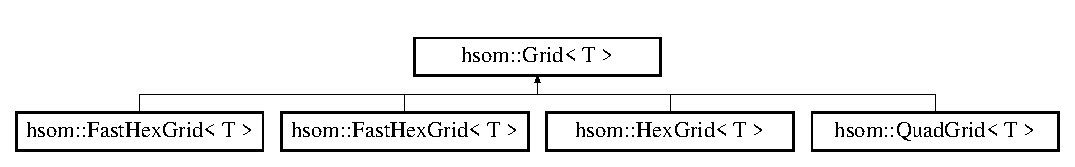
\includegraphics[height=1.794872cm]{classhsom_1_1_grid}
\end{center}
\end{figure}
\subsection*{\-Public \-Member \-Functions}
\begin{DoxyCompactItemize}
\item 
\hypertarget{classhsom_1_1_grid_aba0fb79105155eff14ca1d083af1d406}{\hyperlink{classhsom_1_1_grid_aba0fb79105155eff14ca1d083af1d406}{\-Grid} ()}\label{classhsom_1_1_grid_aba0fb79105155eff14ca1d083af1d406}

\begin{DoxyCompactList}\small\item\em \-Constructs a hex grid with no size information. \end{DoxyCompactList}\item 
\hypertarget{classhsom_1_1_grid_a9d6958c2d779bba109a5db3bc668e32c}{virtual \hyperlink{classhsom_1_1_grid_a9d6958c2d779bba109a5db3bc668e32c}{$\sim$\-Grid} ()}\label{classhsom_1_1_grid_a9d6958c2d779bba109a5db3bc668e32c}

\begin{DoxyCompactList}\small\item\em \-Destructs the \hyperlink{classhsom_1_1_grid}{\-Grid}. \end{DoxyCompactList}\item 
void \hyperlink{classhsom_1_1_grid_a0b78153431550f6261a64085e8fd2f47}{init} (\-Q\-Vector$<$ int $>$ \hyperlink{classhsom_1_1_grid_a3e846473299eb2c7c259659eb61a6234}{size})
\begin{DoxyCompactList}\small\item\em \-Initializes the hex grid with the specified size. \end{DoxyCompactList}\item 
void \hyperlink{classhsom_1_1_grid_a4f786deb4f55e777998b3d7e0c0822e7}{init} (\-Q\-Vector$<$ int $>$ \hyperlink{classhsom_1_1_grid_a3e846473299eb2c7c259659eb61a6234}{size}, \-Q\-Vector$<$ \-T $>$ \hyperlink{classhsom_1_1_grid_ae6b6ffb72e86c3904e8ac21253d85a24}{items})
\begin{DoxyCompactList}\small\item\em \-Initializes the hex grid with the specified size and fills it with the supplied values. \end{DoxyCompactList}\item 
void \hyperlink{classhsom_1_1_grid_ad9ca398c85fd00afc3de894e5bc52dfe}{set\-Items} (\-Q\-Vector$<$ \-T $>$ \hyperlink{classhsom_1_1_grid_ae6b6ffb72e86c3904e8ac21253d85a24}{items})
\begin{DoxyCompactList}\small\item\em \-Sets the items to the supplied items. \end{DoxyCompactList}\item 
\hypertarget{classhsom_1_1_grid_a7f6bd884d4b407dee64985a37fe0bd92}{void \hyperlink{classhsom_1_1_grid_a7f6bd884d4b407dee64985a37fe0bd92}{clear} ()}\label{classhsom_1_1_grid_a7f6bd884d4b407dee64985a37fe0bd92}

\begin{DoxyCompactList}\small\item\em \-Clears the grid. \end{DoxyCompactList}\item 
\hypertarget{classhsom_1_1_grid_ac9b2b7c938d29901e299711151900bbd}{void \hyperlink{classhsom_1_1_grid_ac9b2b7c938d29901e299711151900bbd}{set\-To} (const \-T \&\hyperlink{classhsom_1_1_grid_a991f2eb04dc799ef42c8b58868b9cb8f}{item})}\label{classhsom_1_1_grid_ac9b2b7c938d29901e299711151900bbd}

\begin{DoxyCompactList}\small\item\em \-Sets all of the slots in the grid to the specified item. \end{DoxyCompactList}\item 
\-Q\-Vector$<$ int $>$ \hyperlink{classhsom_1_1_grid_a6bb6f9a0f22054d0d5d39109c3309efd}{neighborhood} (int r, \-Q\-Vector$<$ int $>$ point)
\begin{DoxyCompactList}\small\item\em \-Fetches indices for all slots within a radius of the slot at the given point. \end{DoxyCompactList}\item 
\hypertarget{classhsom_1_1_grid_a7630a12f65349d893d54c9c8ef3b21e9}{virtual void \hyperlink{classhsom_1_1_grid_a7630a12f65349d893d54c9c8ef3b21e9}{set\-Size} (\-Q\-Vector$<$ int $>$ \hyperlink{classhsom_1_1_grid_a3e846473299eb2c7c259659eb61a6234}{size})}\label{classhsom_1_1_grid_a7630a12f65349d893d54c9c8ef3b21e9}

\begin{DoxyCompactList}\small\item\em \-Sets the size of the hex grid. \end{DoxyCompactList}\item 
\hypertarget{classhsom_1_1_grid_a3e846473299eb2c7c259659eb61a6234}{\-Q\-Vector$<$ int $>$ \hyperlink{classhsom_1_1_grid_a3e846473299eb2c7c259659eb61a6234}{size} ()}\label{classhsom_1_1_grid_a3e846473299eb2c7c259659eb61a6234}

\begin{DoxyCompactList}\small\item\em \-Fetches the size of the grid. \end{DoxyCompactList}\item 
\hypertarget{classhsom_1_1_grid_ae77f3109eaa4f66009f90d458bd28ed9}{int \hyperlink{classhsom_1_1_grid_ae77f3109eaa4f66009f90d458bd28ed9}{capacity} ()}\label{classhsom_1_1_grid_ae77f3109eaa4f66009f90d458bd28ed9}

\begin{DoxyCompactList}\small\item\em \-Fetches the linear capacity of the grid. \end{DoxyCompactList}\item 
\hypertarget{classhsom_1_1_grid_ae6b6ffb72e86c3904e8ac21253d85a24}{\-Q\-Vector$<$ \-T $>$ \hyperlink{classhsom_1_1_grid_ae6b6ffb72e86c3904e8ac21253d85a24}{items} ()}\label{classhsom_1_1_grid_ae6b6ffb72e86c3904e8ac21253d85a24}

\begin{DoxyCompactList}\small\item\em \-Fetches the vector of items from this grid. \end{DoxyCompactList}\item 
\-T \& \hyperlink{classhsom_1_1_grid_ac4d7188e7b75823a03a53317656473fa}{operator\mbox{[}$\,$\mbox{]}} (int idx)
\begin{DoxyCompactList}\small\item\em \-Fetches the item at a specific index in the grid. \end{DoxyCompactList}\item 
virtual \-T \& \hyperlink{classhsom_1_1_grid_a991f2eb04dc799ef42c8b58868b9cb8f}{item} (int idx)
\begin{DoxyCompactList}\small\item\em \-Fetches the item at a specific index in the grid. \end{DoxyCompactList}\item 
void \hyperlink{classhsom_1_1_grid_ac61a8700e1e4a3662642d30800046ebb}{check\-Index} (int idx)
\begin{DoxyCompactList}\small\item\em \-Ensures that a given index is valid for this grid. \end{DoxyCompactList}\item 
\-Q\-Vector$<$ \-Q\-Pair$<$ int, int $>$ $>$ \hyperlink{classhsom_1_1_grid_ae957e549123565f3709ad25d9d8c559b}{neighborhood} (int r, int idx)
\begin{DoxyCompactList}\small\item\em \-Fetches indices for all slots within a radius of the specified slot. \end{DoxyCompactList}\item 
\hypertarget{classhsom_1_1_grid_ad45b81e9f494b7d41a8b8a1691be2c8c}{\-Q\-Image \hyperlink{classhsom_1_1_grid_ad45b81e9f494b7d41a8b8a1691be2c8c}{visualize} (double cell\-Radius, \-Q\-Color($\ast$render)(\-T))}\label{classhsom_1_1_grid_ad45b81e9f494b7d41a8b8a1691be2c8c}

\begin{DoxyCompactList}\small\item\em \-Visualizes a hex grid given a function pointer to visualize its contents. \end{DoxyCompactList}\item 
\hypertarget{classhsom_1_1_grid_a785a4cfed83dd7a58fa8bc0b52e852d4}{virtual int \hyperlink{classhsom_1_1_grid_a785a4cfed83dd7a58fa8bc0b52e852d4}{capacity\-From\-Size} (\-Q\-Vector$<$ int $>$ \hyperlink{classhsom_1_1_grid_a3e846473299eb2c7c259659eb61a6234}{size})=0}\label{classhsom_1_1_grid_a785a4cfed83dd7a58fa8bc0b52e852d4}

\begin{DoxyCompactList}\small\item\em \-Gets the capacity of a grid based on the size of the grid. \end{DoxyCompactList}\item 
\hypertarget{classhsom_1_1_grid_a00939983a56d5a2aa8a66b8e1fa8a56d}{virtual void \hyperlink{classhsom_1_1_grid_a00939983a56d5a2aa8a66b8e1fa8a56d}{check\-Size} (\-Q\-Vector$<$ int $>$ \hyperlink{classhsom_1_1_grid_a3e846473299eb2c7c259659eb61a6234}{size})=0}\label{classhsom_1_1_grid_a00939983a56d5a2aa8a66b8e1fa8a56d}

\begin{DoxyCompactList}\small\item\em \-Checks the supplied size to ensure that it is valid for the \hyperlink{classhsom_1_1_grid}{\-Grid}. \end{DoxyCompactList}\item 
virtual void \hyperlink{classhsom_1_1_grid_abf12e08a06d3ad123ac7fcb72c04aae6}{check\-Coords} (\-Q\-Vector$<$ int $>$ \hyperlink{classhsom_1_1_grid_a4a68c15ff3ffcd052bff769e4d9e899b}{coords})=0
\begin{DoxyCompactList}\small\item\em \-Checks a given point to ensure it is a valid reference to an element in the grid. \end{DoxyCompactList}\item 
virtual int \hyperlink{classhsom_1_1_grid_a1c3162ea843ab3f7e79136425e011a5d}{index} (\-Q\-Vector$<$ int $>$ \hyperlink{classhsom_1_1_grid_a4a68c15ff3ffcd052bff769e4d9e899b}{coords})=0
\begin{DoxyCompactList}\small\item\em \-Fetches the index for the slot at the specified coordinates. \end{DoxyCompactList}\item 
virtual \-Q\-Vector$<$ int $>$ \hyperlink{classhsom_1_1_grid_a4a68c15ff3ffcd052bff769e4d9e899b}{coords} (int idx)=0
\begin{DoxyCompactList}\small\item\em \-Fetches the coordinates given an index. \end{DoxyCompactList}\item 
\hypertarget{classhsom_1_1_grid_acc0364a698525d1239a7042eb01f79e6}{virtual int \hyperlink{classhsom_1_1_grid_acc0364a698525d1239a7042eb01f79e6}{diagonal} ()=0}\label{classhsom_1_1_grid_acc0364a698525d1239a7042eb01f79e6}

\begin{DoxyCompactList}\small\item\em \-Fetches the length of the major diagonal running through the grid. \end{DoxyCompactList}\item 
\hypertarget{classhsom_1_1_grid_a91c2fe63cf5fdc2a9f82b4a09a7e0722}{virtual int \hyperlink{classhsom_1_1_grid_a91c2fe63cf5fdc2a9f82b4a09a7e0722}{distance} (int idx0, int idx1)=0}\label{classhsom_1_1_grid_a91c2fe63cf5fdc2a9f82b4a09a7e0722}

\begin{DoxyCompactList}\small\item\em \-Fetches the distance between two cells in the grid. \end{DoxyCompactList}\item 
\hypertarget{classhsom_1_1_grid_aadbdeb2f305d8549998866397450732f}{virtual \-Q\-Vector$<$ double $>$ \hyperlink{classhsom_1_1_grid_aadbdeb2f305d8549998866397450732f}{real\-Bounds} ()=0}\label{classhsom_1_1_grid_aadbdeb2f305d8549998866397450732f}

\begin{DoxyCompactList}\small\item\em \-Fetches the extents of the real coordinate mapping space ( should only be used for visualization ) \end{DoxyCompactList}\item 
\hypertarget{classhsom_1_1_grid_a9a40aeb6a5aea850e576224281f63504}{virtual \-Q\-Vector$<$ double $>$ \hyperlink{classhsom_1_1_grid_a9a40aeb6a5aea850e576224281f63504}{real\-Coords} (int idx)=0}\label{classhsom_1_1_grid_a9a40aeb6a5aea850e576224281f63504}

\begin{DoxyCompactList}\small\item\em \-Fetches the real coordinates of a given index in the grid ( should only be used for visualization ) \end{DoxyCompactList}\end{DoxyCompactItemize}
\subsection*{\-Protected \-Member \-Functions}
\begin{DoxyCompactItemize}
\item 
\hypertarget{classhsom_1_1_grid_a1a96dd2d3bfc55ab6968a55bc457460f}{void \hyperlink{classhsom_1_1_grid_a1a96dd2d3bfc55ab6968a55bc457460f}{set\-Capacity} (int \hyperlink{classhsom_1_1_grid_ae77f3109eaa4f66009f90d458bd28ed9}{capacity})}\label{classhsom_1_1_grid_a1a96dd2d3bfc55ab6968a55bc457460f}

\begin{DoxyCompactList}\small\item\em \-Sets the size of the grid. \end{DoxyCompactList}\end{DoxyCompactItemize}
\subsection*{\-Protected \-Attributes}
\begin{DoxyCompactItemize}
\item 
\hypertarget{classhsom_1_1_grid_a8d8e32e70c111bc5476d83f6f1837ed4}{\-Q\-Vector$<$ int $>$ \hyperlink{classhsom_1_1_grid_a8d8e32e70c111bc5476d83f6f1837ed4}{\-\_\-size}}\label{classhsom_1_1_grid_a8d8e32e70c111bc5476d83f6f1837ed4}

\begin{DoxyCompactList}\small\item\em \-A vector describing the size of the grid. \end{DoxyCompactList}\end{DoxyCompactItemize}
\subsubsection*{template$<$class \-T$>$ class hsom\-::\-Grid$<$ T $>$}



\subsection{\-Member \-Function \-Documentation}
\hypertarget{classhsom_1_1_grid_abf12e08a06d3ad123ac7fcb72c04aae6}{\index{hsom\-::\-Grid@{hsom\-::\-Grid}!check\-Coords@{check\-Coords}}
\index{check\-Coords@{check\-Coords}!hsom::Grid@{hsom\-::\-Grid}}
\subsubsection[{check\-Coords}]{\setlength{\rightskip}{0pt plus 5cm}template$<$class \-T$>$ virtual void {\bf hsom\-::\-Grid}$<$ \-T $>$\-::{\bf check\-Coords} (
\begin{DoxyParamCaption}
\item[{\-Q\-Vector$<$ int $>$}]{coords}
\end{DoxyParamCaption}
)\hspace{0.3cm}{\ttfamily  \mbox{[}pure virtual\mbox{]}}}}\label{classhsom_1_1_grid_abf12e08a06d3ad123ac7fcb72c04aae6}


\-Checks a given point to ensure it is a valid reference to an element in the grid. 


\begin{DoxyParams}{\-Parameters}
{\em coords} & \-The point in the grid for which to check for validity \\
\hline
\end{DoxyParams}


\-Implemented in \hyperlink{classhsom_1_1_hex_grid_a9fb21460ce970fdd8d3075ead9db49a7}{hsom\-::\-Hex\-Grid$<$ T $>$}, \hyperlink{classhsom_1_1_hex_grid_a9fb21460ce970fdd8d3075ead9db49a7}{hsom\-::\-Hex\-Grid$<$ double $>$}, \hyperlink{classhsom_1_1_quad_grid_a73f94c48b7544917753883ccd813c9e6}{hsom\-::\-Quad\-Grid$<$ T $>$}, \hyperlink{classhsom_1_1_fast_hex_grid_a8617bee85643b77b31b54644f019ceb3}{hsom\-::\-Fast\-Hex\-Grid$<$ T $>$}, and \hyperlink{classhsom_1_1_fast_hex_grid_a8617bee85643b77b31b54644f019ceb3}{hsom\-::\-Fast\-Hex\-Grid$<$ T $>$}.

\hypertarget{classhsom_1_1_grid_ac61a8700e1e4a3662642d30800046ebb}{\index{hsom\-::\-Grid@{hsom\-::\-Grid}!check\-Index@{check\-Index}}
\index{check\-Index@{check\-Index}!hsom::Grid@{hsom\-::\-Grid}}
\subsubsection[{check\-Index}]{\setlength{\rightskip}{0pt plus 5cm}template$<$class \-T$>$ void {\bf hsom\-::\-Grid}$<$ \-T $>$\-::{\bf check\-Index} (
\begin{DoxyParamCaption}
\item[{int}]{idx}
\end{DoxyParamCaption}
)\hspace{0.3cm}{\ttfamily  \mbox{[}inline\mbox{]}}}}\label{classhsom_1_1_grid_ac61a8700e1e4a3662642d30800046ebb}


\-Ensures that a given index is valid for this grid. 


\begin{DoxyParams}{\-Parameters}
{\em idx} & \-The index to check for validity \\
\hline
\end{DoxyParams}
\hypertarget{classhsom_1_1_grid_a4a68c15ff3ffcd052bff769e4d9e899b}{\index{hsom\-::\-Grid@{hsom\-::\-Grid}!coords@{coords}}
\index{coords@{coords}!hsom::Grid@{hsom\-::\-Grid}}
\subsubsection[{coords}]{\setlength{\rightskip}{0pt plus 5cm}template$<$class \-T$>$ virtual \-Q\-Vector$<$int$>$ {\bf hsom\-::\-Grid}$<$ \-T $>$\-::{\bf coords} (
\begin{DoxyParamCaption}
\item[{int}]{idx}
\end{DoxyParamCaption}
)\hspace{0.3cm}{\ttfamily  \mbox{[}pure virtual\mbox{]}}}}\label{classhsom_1_1_grid_a4a68c15ff3ffcd052bff769e4d9e899b}


\-Fetches the coordinates given an index. 


\begin{DoxyParams}{\-Parameters}
{\em idx} & \-The index in the grid for which to fetch the coordinates \\
\hline
\end{DoxyParams}


\-Implemented in \hyperlink{classhsom_1_1_hex_grid_a2016e6d1a0e8b01a705a7d9040797329}{hsom\-::\-Hex\-Grid$<$ T $>$}, \hyperlink{classhsom_1_1_hex_grid_a2016e6d1a0e8b01a705a7d9040797329}{hsom\-::\-Hex\-Grid$<$ double $>$}, \hyperlink{classhsom_1_1_quad_grid_a8f91269433c403a6034efdec7e97104b}{hsom\-::\-Quad\-Grid$<$ T $>$}, \hyperlink{classhsom_1_1_fast_hex_grid_a5305b83a2932122381f5c78a162cd147}{hsom\-::\-Fast\-Hex\-Grid$<$ T $>$}, and \hyperlink{classhsom_1_1_fast_hex_grid_a5305b83a2932122381f5c78a162cd147}{hsom\-::\-Fast\-Hex\-Grid$<$ T $>$}.

\hypertarget{classhsom_1_1_grid_a1c3162ea843ab3f7e79136425e011a5d}{\index{hsom\-::\-Grid@{hsom\-::\-Grid}!index@{index}}
\index{index@{index}!hsom::Grid@{hsom\-::\-Grid}}
\subsubsection[{index}]{\setlength{\rightskip}{0pt plus 5cm}template$<$class \-T$>$ virtual int {\bf hsom\-::\-Grid}$<$ \-T $>$\-::{\bf index} (
\begin{DoxyParamCaption}
\item[{\-Q\-Vector$<$ int $>$}]{coords}
\end{DoxyParamCaption}
)\hspace{0.3cm}{\ttfamily  \mbox{[}pure virtual\mbox{]}}}}\label{classhsom_1_1_grid_a1c3162ea843ab3f7e79136425e011a5d}


\-Fetches the index for the slot at the specified coordinates. 


\begin{DoxyParams}{\-Parameters}
{\em coords} & \-The point in the grid for which to fetch the index \\
\hline
\end{DoxyParams}


\-Implemented in \hyperlink{classhsom_1_1_hex_grid_a2fdc90350afd51ac994726ca5f161698}{hsom\-::\-Hex\-Grid$<$ T $>$}, \hyperlink{classhsom_1_1_hex_grid_a2fdc90350afd51ac994726ca5f161698}{hsom\-::\-Hex\-Grid$<$ double $>$}, \hyperlink{classhsom_1_1_quad_grid_a5623e24a82df043cec092e5cb61aed34}{hsom\-::\-Quad\-Grid$<$ T $>$}, \hyperlink{classhsom_1_1_fast_hex_grid_a74ef97079e75235a07f9dc70bdbf238a}{hsom\-::\-Fast\-Hex\-Grid$<$ T $>$}, and \hyperlink{classhsom_1_1_fast_hex_grid_a74ef97079e75235a07f9dc70bdbf238a}{hsom\-::\-Fast\-Hex\-Grid$<$ T $>$}.

\hypertarget{classhsom_1_1_grid_a0b78153431550f6261a64085e8fd2f47}{\index{hsom\-::\-Grid@{hsom\-::\-Grid}!init@{init}}
\index{init@{init}!hsom::Grid@{hsom\-::\-Grid}}
\subsubsection[{init}]{\setlength{\rightskip}{0pt plus 5cm}template$<$class \-T$>$ void {\bf hsom\-::\-Grid}$<$ \-T $>$\-::{\bf init} (
\begin{DoxyParamCaption}
\item[{\-Q\-Vector$<$ int $>$}]{size}
\end{DoxyParamCaption}
)\hspace{0.3cm}{\ttfamily  \mbox{[}inline\mbox{]}}}}\label{classhsom_1_1_grid_a0b78153431550f6261a64085e8fd2f47}


\-Initializes the hex grid with the specified size. 


\begin{DoxyParams}{\-Parameters}
{\em size} & \-The size of grid to create \\
\hline
\end{DoxyParams}
\hypertarget{classhsom_1_1_grid_a4f786deb4f55e777998b3d7e0c0822e7}{\index{hsom\-::\-Grid@{hsom\-::\-Grid}!init@{init}}
\index{init@{init}!hsom::Grid@{hsom\-::\-Grid}}
\subsubsection[{init}]{\setlength{\rightskip}{0pt plus 5cm}template$<$class \-T$>$ void {\bf hsom\-::\-Grid}$<$ \-T $>$\-::{\bf init} (
\begin{DoxyParamCaption}
\item[{\-Q\-Vector$<$ int $>$}]{size, }
\item[{\-Q\-Vector$<$ \-T $>$}]{items}
\end{DoxyParamCaption}
)\hspace{0.3cm}{\ttfamily  \mbox{[}inline\mbox{]}}}}\label{classhsom_1_1_grid_a4f786deb4f55e777998b3d7e0c0822e7}


\-Initializes the hex grid with the specified size and fills it with the supplied values. 


\begin{DoxyParams}{\-Parameters}
{\em size} & \-The size of grid to create \\
\hline
{\em items} & \-The items with which to populate the grid \\
\hline
\end{DoxyParams}
\hypertarget{classhsom_1_1_grid_a991f2eb04dc799ef42c8b58868b9cb8f}{\index{hsom\-::\-Grid@{hsom\-::\-Grid}!item@{item}}
\index{item@{item}!hsom::Grid@{hsom\-::\-Grid}}
\subsubsection[{item}]{\setlength{\rightskip}{0pt plus 5cm}template$<$class \-T$>$ virtual \-T\& {\bf hsom\-::\-Grid}$<$ \-T $>$\-::{\bf item} (
\begin{DoxyParamCaption}
\item[{int}]{idx}
\end{DoxyParamCaption}
)\hspace{0.3cm}{\ttfamily  \mbox{[}inline, virtual\mbox{]}}}}\label{classhsom_1_1_grid_a991f2eb04dc799ef42c8b58868b9cb8f}


\-Fetches the item at a specific index in the grid. 


\begin{DoxyParams}{\-Parameters}
{\em idx} & \-The index in the grid from which to fetch an item \\
\hline
\end{DoxyParams}
\hypertarget{classhsom_1_1_grid_a6bb6f9a0f22054d0d5d39109c3309efd}{\index{hsom\-::\-Grid@{hsom\-::\-Grid}!neighborhood@{neighborhood}}
\index{neighborhood@{neighborhood}!hsom::Grid@{hsom\-::\-Grid}}
\subsubsection[{neighborhood}]{\setlength{\rightskip}{0pt plus 5cm}template$<$class \-T$>$ \-Q\-Vector$<$int$>$ {\bf hsom\-::\-Grid}$<$ \-T $>$\-::{\bf neighborhood} (
\begin{DoxyParamCaption}
\item[{int}]{r, }
\item[{\-Q\-Vector$<$ int $>$}]{point}
\end{DoxyParamCaption}
)\hspace{0.3cm}{\ttfamily  \mbox{[}inline\mbox{]}}}}\label{classhsom_1_1_grid_a6bb6f9a0f22054d0d5d39109c3309efd}


\-Fetches indices for all slots within a radius of the slot at the given point. 


\begin{DoxyParams}{\-Parameters}
{\em r} & \-The radius within which a cell must lie to be part of the neighborhood \\
\hline
{\em point} & \-The origin cell for the neighborhood ( center cell ) \\
\hline
\end{DoxyParams}
\hypertarget{classhsom_1_1_grid_ae957e549123565f3709ad25d9d8c559b}{\index{hsom\-::\-Grid@{hsom\-::\-Grid}!neighborhood@{neighborhood}}
\index{neighborhood@{neighborhood}!hsom::Grid@{hsom\-::\-Grid}}
\subsubsection[{neighborhood}]{\setlength{\rightskip}{0pt plus 5cm}template$<$class \-T$>$ \-Q\-Vector$<$ \-Q\-Pair$<$int, int$>$ $>$ {\bf hsom\-::\-Grid}$<$ \-T $>$\-::{\bf neighborhood} (
\begin{DoxyParamCaption}
\item[{int}]{r, }
\item[{int}]{idx}
\end{DoxyParamCaption}
)\hspace{0.3cm}{\ttfamily  \mbox{[}inline\mbox{]}}}}\label{classhsom_1_1_grid_ae957e549123565f3709ad25d9d8c559b}


\-Fetches indices for all slots within a radius of the specified slot. 


\begin{DoxyParams}{\-Parameters}
{\em r} & \-The radius within which a cell must lie to be a part of the neighborhood \\
\hline
{\em idx} & \-The origin index for the neighborhood ( center cell ) \\
\hline
\end{DoxyParams}
\hypertarget{classhsom_1_1_grid_ac4d7188e7b75823a03a53317656473fa}{\index{hsom\-::\-Grid@{hsom\-::\-Grid}!operator\mbox{[}$\,$\mbox{]}@{operator[]}}
\index{operator\mbox{[}$\,$\mbox{]}@{operator[]}!hsom::Grid@{hsom\-::\-Grid}}
\subsubsection[{operator[]}]{\setlength{\rightskip}{0pt plus 5cm}template$<$class \-T$>$ \-T\& {\bf hsom\-::\-Grid}$<$ \-T $>$\-::operator\mbox{[}$\,$\mbox{]} (
\begin{DoxyParamCaption}
\item[{int}]{idx}
\end{DoxyParamCaption}
)\hspace{0.3cm}{\ttfamily  \mbox{[}inline\mbox{]}}}}\label{classhsom_1_1_grid_ac4d7188e7b75823a03a53317656473fa}


\-Fetches the item at a specific index in the grid. 

\begin{DoxyRefDesc}{\-Todo}
\item[\hyperlink{todo__todo000007}{\-Todo}]\-Add a bounds checking here and custom exceptions would be nice \end{DoxyRefDesc}

\begin{DoxyParams}{\-Parameters}
{\em idx} & \-The index in the grid from which to fetch an item \\
\hline
\end{DoxyParams}
\hypertarget{classhsom_1_1_grid_ad9ca398c85fd00afc3de894e5bc52dfe}{\index{hsom\-::\-Grid@{hsom\-::\-Grid}!set\-Items@{set\-Items}}
\index{set\-Items@{set\-Items}!hsom::Grid@{hsom\-::\-Grid}}
\subsubsection[{set\-Items}]{\setlength{\rightskip}{0pt plus 5cm}template$<$class \-T$>$ void {\bf hsom\-::\-Grid}$<$ \-T $>$\-::{\bf set\-Items} (
\begin{DoxyParamCaption}
\item[{\-Q\-Vector$<$ \-T $>$}]{items}
\end{DoxyParamCaption}
)\hspace{0.3cm}{\ttfamily  \mbox{[}inline\mbox{]}}}}\label{classhsom_1_1_grid_ad9ca398c85fd00afc3de894e5bc52dfe}


\-Sets the items to the supplied items. 


\begin{DoxyParams}{\-Parameters}
{\em items} & \-The items with which to populate the grid \\
\hline
\end{DoxyParams}


\-The documentation for this class was generated from the following file\-:\begin{DoxyCompactItemize}
\item 
\-C\-:/\-Users/d3x874/\-Documents/source/urania/grids/grid.\-hpp\end{DoxyCompactItemize}

\hypertarget{classhsom_1_1_hex_grid}{\section{hsom\-:\-:\-Hex\-Grid$<$ \-T $>$ \-Class \-Template \-Reference}
\label{classhsom_1_1_hex_grid}\index{hsom\-::\-Hex\-Grid$<$ T $>$@{hsom\-::\-Hex\-Grid$<$ T $>$}}
}


{\ttfamily \#include $<$hexgrid.\-hpp$>$}

\-Inheritance diagram for hsom\-:\-:\-Hex\-Grid$<$ \-T $>$\-:\begin{figure}[H]
\begin{center}
\leavevmode
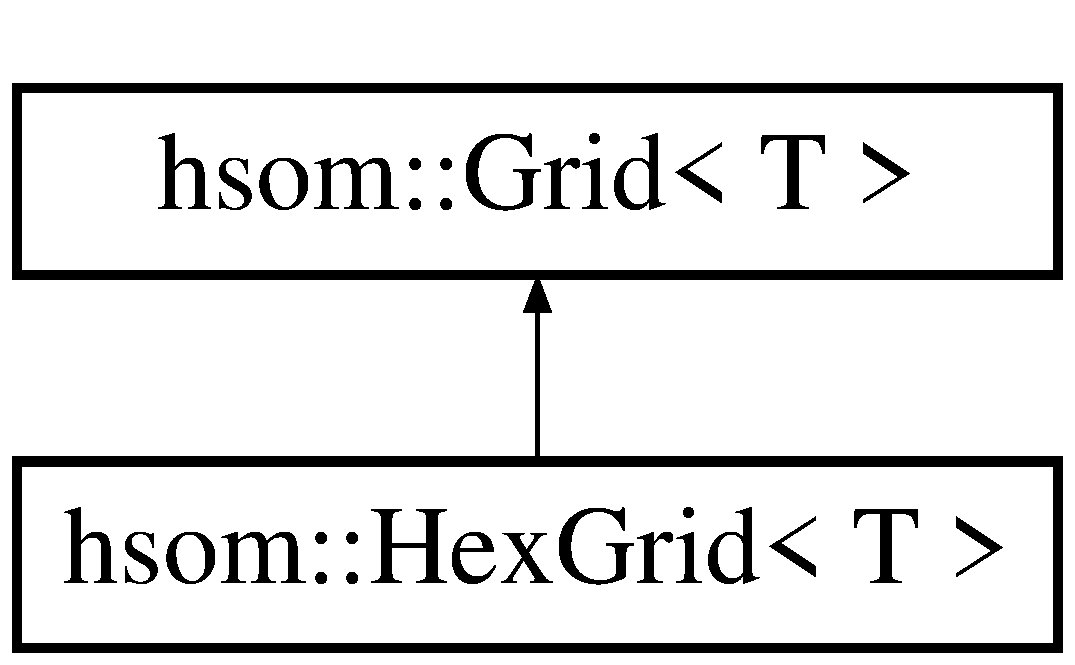
\includegraphics[height=2.000000cm]{classhsom_1_1_hex_grid}
\end{center}
\end{figure}
\subsection*{\-Public \-Member \-Functions}
\begin{DoxyCompactItemize}
\item 
\hypertarget{classhsom_1_1_hex_grid_a561fff2cdd479c0ea385229d47ae0de8}{\hyperlink{classhsom_1_1_hex_grid_a561fff2cdd479c0ea385229d47ae0de8}{\-Hex\-Grid} ()}\label{classhsom_1_1_hex_grid_a561fff2cdd479c0ea385229d47ae0de8}

\begin{DoxyCompactList}\small\item\em \-Constructs a hex grid with no size information. \end{DoxyCompactList}\item 
\hyperlink{classhsom_1_1_hex_grid_a116810466306642ff20c1f5a47d2fcdc}{\-Hex\-Grid} (\-Q\-Vector$<$ int $>$ \hyperlink{classhsom_1_1_grid_a3e846473299eb2c7c259659eb61a6234}{size})
\begin{DoxyCompactList}\small\item\em \-Constructs the hex grid with a specified size. \end{DoxyCompactList}\item 
\hyperlink{classhsom_1_1_hex_grid_a6ec57bd99b207a2de3b5464f363aefef}{\-Hex\-Grid} (int w, int h)
\begin{DoxyCompactList}\small\item\em \-Constructs the hex grid with a specified size. \end{DoxyCompactList}\item 
\hyperlink{classhsom_1_1_hex_grid_a9ba65c149bec76393d7c20b746f1b023}{\-Hex\-Grid} (\-Q\-Vector$<$ int $>$ \hyperlink{classhsom_1_1_grid_a3e846473299eb2c7c259659eb61a6234}{size}, \-Q\-Vector$<$ \-T $>$ \hyperlink{classhsom_1_1_grid_ae6b6ffb72e86c3904e8ac21253d85a24}{items})
\begin{DoxyCompactList}\small\item\em \-Constructs the hex grid with the specified size and fills it with the supplied values. \end{DoxyCompactList}\item 
\hyperlink{classhsom_1_1_hex_grid_a204c75cb7144f624a1456dd47eb93efe}{\-Hex\-Grid} (int w, int h, \-Q\-Vector$<$ \-T $>$ \hyperlink{classhsom_1_1_grid_ae6b6ffb72e86c3904e8ac21253d85a24}{items})
\begin{DoxyCompactList}\small\item\em \-Constructs the hex grid with the specified size and fills it with the supplied values. \end{DoxyCompactList}\item 
\hypertarget{classhsom_1_1_hex_grid_a7a5cec068de3378626aab09127f844c5}{virtual \hyperlink{classhsom_1_1_hex_grid_a7a5cec068de3378626aab09127f844c5}{$\sim$\-Hex\-Grid} ()}\label{classhsom_1_1_hex_grid_a7a5cec068de3378626aab09127f844c5}

\begin{DoxyCompactList}\small\item\em \-Destructs the \hyperlink{classhsom_1_1_hex_grid}{\-Hex\-Grid}. \end{DoxyCompactList}\item 
\hypertarget{classhsom_1_1_hex_grid_a2c1dfa6a6ecf7b75233aceb4384de4e0}{int {\bfseries w} ()}\label{classhsom_1_1_hex_grid_a2c1dfa6a6ecf7b75233aceb4384de4e0}

\item 
\hypertarget{classhsom_1_1_hex_grid_a28440198319e03676056109c7f89a43f}{int {\bfseries h} ()}\label{classhsom_1_1_hex_grid_a28440198319e03676056109c7f89a43f}

\item 
\hypertarget{classhsom_1_1_hex_grid_a614c32e28e2bf67015490c2e66bfb5c1}{virtual void \hyperlink{classhsom_1_1_hex_grid_a614c32e28e2bf67015490c2e66bfb5c1}{check\-Size} (\-Q\-Vector$<$ int $>$ \hyperlink{classhsom_1_1_grid_a3e846473299eb2c7c259659eb61a6234}{size})}\label{classhsom_1_1_hex_grid_a614c32e28e2bf67015490c2e66bfb5c1}

\begin{DoxyCompactList}\small\item\em \-Checks the supplied size to ensure that it is valid for the \hyperlink{classhsom_1_1_hex_grid}{\-Hex\-Grid}. \end{DoxyCompactList}\item 
\hypertarget{classhsom_1_1_hex_grid_a782533d1c9c15f1da2f0b9c7af44c48d}{virtual int \hyperlink{classhsom_1_1_hex_grid_a782533d1c9c15f1da2f0b9c7af44c48d}{capacity\-From\-Size} (\-Q\-Vector$<$ int $>$ \hyperlink{classhsom_1_1_grid_a3e846473299eb2c7c259659eb61a6234}{size})}\label{classhsom_1_1_hex_grid_a782533d1c9c15f1da2f0b9c7af44c48d}

\begin{DoxyCompactList}\small\item\em \-Gets the capacity of a grid based on the size of the grid. \end{DoxyCompactList}\item 
\hypertarget{classhsom_1_1_hex_grid_a9fb21460ce970fdd8d3075ead9db49a7}{virtual void \hyperlink{classhsom_1_1_hex_grid_a9fb21460ce970fdd8d3075ead9db49a7}{check\-Coords} (\-Q\-Vector$<$ int $>$ \hyperlink{classhsom_1_1_hex_grid_a2016e6d1a0e8b01a705a7d9040797329}{coords})}\label{classhsom_1_1_hex_grid_a9fb21460ce970fdd8d3075ead9db49a7}

\begin{DoxyCompactList}\small\item\em \-Checks a given point to ensure it is a valid reference to an element in the grid. \end{DoxyCompactList}\item 
virtual int \hyperlink{classhsom_1_1_hex_grid_a2fdc90350afd51ac994726ca5f161698}{index} (\-Q\-Vector$<$ int $>$ \hyperlink{classhsom_1_1_hex_grid_a2016e6d1a0e8b01a705a7d9040797329}{coords})
\begin{DoxyCompactList}\small\item\em \-Fetches the index for the slot at the specified coordinates. \end{DoxyCompactList}\item 
virtual \-Q\-Vector$<$ int $>$ \hyperlink{classhsom_1_1_hex_grid_a2016e6d1a0e8b01a705a7d9040797329}{coords} (int idx)
\begin{DoxyCompactList}\small\item\em \-Fetches the coordinates given an index. \end{DoxyCompactList}\item 
\hypertarget{classhsom_1_1_hex_grid_ad74b8e5fe63c4d41d4b531a7fe95163c}{virtual \-Q\-Vector$<$ double $>$ \hyperlink{classhsom_1_1_hex_grid_ad74b8e5fe63c4d41d4b531a7fe95163c}{real\-Bounds} ()}\label{classhsom_1_1_hex_grid_ad74b8e5fe63c4d41d4b531a7fe95163c}

\begin{DoxyCompactList}\small\item\em \-Fetches the extents of the real coordinate mapping space ( should only be used for visualization ) \end{DoxyCompactList}\item 
\hypertarget{classhsom_1_1_hex_grid_afb2e7dc46222030dceea28e35eff2a06}{virtual \-Q\-Vector$<$ double $>$ \hyperlink{classhsom_1_1_hex_grid_afb2e7dc46222030dceea28e35eff2a06}{real\-Coords} (int idx)}\label{classhsom_1_1_hex_grid_afb2e7dc46222030dceea28e35eff2a06}

\begin{DoxyCompactList}\small\item\em \-Fetches the real coordinates of a given index in the grid ( should only be used for visualization ) \end{DoxyCompactList}\item 
virtual int \hyperlink{classhsom_1_1_hex_grid_aa1fe9291ee1c82da00bca12b906959cb}{diagonal} ()
\begin{DoxyCompactList}\small\item\em \-Fetches the length of the major diagonal running through the grid. \end{DoxyCompactList}\item 
\hypertarget{classhsom_1_1_hex_grid_ad926d9db99d77cc238536de4dbb427d9}{virtual int \hyperlink{classhsom_1_1_hex_grid_ad926d9db99d77cc238536de4dbb427d9}{distance} (int idx0, int idx1)}\label{classhsom_1_1_hex_grid_ad926d9db99d77cc238536de4dbb427d9}

\begin{DoxyCompactList}\small\item\em \-Fetches indices for all slots within a radius of the specified slot. \end{DoxyCompactList}\end{DoxyCompactItemize}


\subsection{\-Detailed \-Description}
\subsubsection*{template$<$class \-T$>$class hsom\-::\-Hex\-Grid$<$ T $>$}

\-The \hyperlink{classhsom_1_1_hex_grid}{\-Hex\-Grid} class provides the basis for the spatial organization of the \-Self \-Organizing \-Map. \-It provides a hexagonal grid which supports neighborhood searches, edge wrapping, and other functionality. 

\subsection{\-Constructor \& \-Destructor \-Documentation}
\hypertarget{classhsom_1_1_hex_grid_a116810466306642ff20c1f5a47d2fcdc}{\index{hsom\-::\-Hex\-Grid@{hsom\-::\-Hex\-Grid}!\-Hex\-Grid@{\-Hex\-Grid}}
\index{\-Hex\-Grid@{\-Hex\-Grid}!hsom::HexGrid@{hsom\-::\-Hex\-Grid}}
\subsubsection[{\-Hex\-Grid}]{\setlength{\rightskip}{0pt plus 5cm}template$<$class \-T$>$ {\bf hsom\-::\-Hex\-Grid}$<$ \-T $>$\-::{\bf \-Hex\-Grid} (
\begin{DoxyParamCaption}
\item[{\-Q\-Vector$<$ int $>$}]{size}
\end{DoxyParamCaption}
)\hspace{0.3cm}{\ttfamily  \mbox{[}inline\mbox{]}}}}\label{classhsom_1_1_hex_grid_a116810466306642ff20c1f5a47d2fcdc}


\-Constructs the hex grid with a specified size. 


\begin{DoxyParams}{\-Parameters}
{\em size} & \-The size of the new grid \\
\hline
\end{DoxyParams}
\hypertarget{classhsom_1_1_hex_grid_a6ec57bd99b207a2de3b5464f363aefef}{\index{hsom\-::\-Hex\-Grid@{hsom\-::\-Hex\-Grid}!\-Hex\-Grid@{\-Hex\-Grid}}
\index{\-Hex\-Grid@{\-Hex\-Grid}!hsom::HexGrid@{hsom\-::\-Hex\-Grid}}
\subsubsection[{\-Hex\-Grid}]{\setlength{\rightskip}{0pt plus 5cm}template$<$class \-T$>$ {\bf hsom\-::\-Hex\-Grid}$<$ \-T $>$\-::{\bf \-Hex\-Grid} (
\begin{DoxyParamCaption}
\item[{int}]{w, }
\item[{int}]{h}
\end{DoxyParamCaption}
)\hspace{0.3cm}{\ttfamily  \mbox{[}inline\mbox{]}}}}\label{classhsom_1_1_hex_grid_a6ec57bd99b207a2de3b5464f363aefef}


\-Constructs the hex grid with a specified size. 


\begin{DoxyParams}{\-Parameters}
{\em w} & \-The width of the hex grid \\
\hline
{\em h} & \-The height of the hex grid \\
\hline
\end{DoxyParams}
\hypertarget{classhsom_1_1_hex_grid_a9ba65c149bec76393d7c20b746f1b023}{\index{hsom\-::\-Hex\-Grid@{hsom\-::\-Hex\-Grid}!\-Hex\-Grid@{\-Hex\-Grid}}
\index{\-Hex\-Grid@{\-Hex\-Grid}!hsom::HexGrid@{hsom\-::\-Hex\-Grid}}
\subsubsection[{\-Hex\-Grid}]{\setlength{\rightskip}{0pt plus 5cm}template$<$class \-T$>$ {\bf hsom\-::\-Hex\-Grid}$<$ \-T $>$\-::{\bf \-Hex\-Grid} (
\begin{DoxyParamCaption}
\item[{\-Q\-Vector$<$ int $>$}]{size, }
\item[{\-Q\-Vector$<$ \-T $>$}]{items}
\end{DoxyParamCaption}
)\hspace{0.3cm}{\ttfamily  \mbox{[}inline\mbox{]}}}}\label{classhsom_1_1_hex_grid_a9ba65c149bec76393d7c20b746f1b023}


\-Constructs the hex grid with the specified size and fills it with the supplied values. 


\begin{DoxyParams}{\-Parameters}
{\em size} & \-The size of the new grid \\
\hline
{\em items} & \-The items with which to populate the grid \\
\hline
\end{DoxyParams}
\hypertarget{classhsom_1_1_hex_grid_a204c75cb7144f624a1456dd47eb93efe}{\index{hsom\-::\-Hex\-Grid@{hsom\-::\-Hex\-Grid}!\-Hex\-Grid@{\-Hex\-Grid}}
\index{\-Hex\-Grid@{\-Hex\-Grid}!hsom::HexGrid@{hsom\-::\-Hex\-Grid}}
\subsubsection[{\-Hex\-Grid}]{\setlength{\rightskip}{0pt plus 5cm}template$<$class \-T$>$ {\bf hsom\-::\-Hex\-Grid}$<$ \-T $>$\-::{\bf \-Hex\-Grid} (
\begin{DoxyParamCaption}
\item[{int}]{w, }
\item[{int}]{h, }
\item[{\-Q\-Vector$<$ \-T $>$}]{items}
\end{DoxyParamCaption}
)\hspace{0.3cm}{\ttfamily  \mbox{[}inline\mbox{]}}}}\label{classhsom_1_1_hex_grid_a204c75cb7144f624a1456dd47eb93efe}


\-Constructs the hex grid with the specified size and fills it with the supplied values. 


\begin{DoxyParams}{\-Parameters}
{\em w} & \-The width of the hex grid \\
\hline
{\em h} & \-The height of the hex grid \\
\hline
{\em items} & \-The items with which to populate the grid \\
\hline
\end{DoxyParams}


\subsection{\-Member \-Function \-Documentation}
\hypertarget{classhsom_1_1_hex_grid_a2016e6d1a0e8b01a705a7d9040797329}{\index{hsom\-::\-Hex\-Grid@{hsom\-::\-Hex\-Grid}!coords@{coords}}
\index{coords@{coords}!hsom::HexGrid@{hsom\-::\-Hex\-Grid}}
\subsubsection[{coords}]{\setlength{\rightskip}{0pt plus 5cm}template$<$class \-T$>$ virtual \-Q\-Vector$<$int$>$ {\bf hsom\-::\-Hex\-Grid}$<$ \-T $>$\-::{\bf coords} (
\begin{DoxyParamCaption}
\item[{int}]{idx}
\end{DoxyParamCaption}
)\hspace{0.3cm}{\ttfamily  \mbox{[}inline, virtual\mbox{]}}}}\label{classhsom_1_1_hex_grid_a2016e6d1a0e8b01a705a7d9040797329}


\-Fetches the coordinates given an index. 


\begin{DoxyParams}{\-Parameters}
{\em idx} & \-The index in the grid for which to fetch the coordinates \\
\hline
\end{DoxyParams}


\-Implements \hyperlink{classhsom_1_1_grid_a4a68c15ff3ffcd052bff769e4d9e899b}{hsom\-::\-Grid$<$ T $>$}.

\hypertarget{classhsom_1_1_hex_grid_aa1fe9291ee1c82da00bca12b906959cb}{\index{hsom\-::\-Hex\-Grid@{hsom\-::\-Hex\-Grid}!diagonal@{diagonal}}
\index{diagonal@{diagonal}!hsom::HexGrid@{hsom\-::\-Hex\-Grid}}
\subsubsection[{diagonal}]{\setlength{\rightskip}{0pt plus 5cm}template$<$class \-T$>$ virtual int {\bf hsom\-::\-Hex\-Grid}$<$ \-T $>$\-::{\bf diagonal} (
\begin{DoxyParamCaption}
{}
\end{DoxyParamCaption}
)\hspace{0.3cm}{\ttfamily  \mbox{[}inline, virtual\mbox{]}}}}\label{classhsom_1_1_hex_grid_aa1fe9291ee1c82da00bca12b906959cb}


\-Fetches the length of the major diagonal running through the grid. 

\begin{DoxyRefDesc}{\-Todo}
\item[\hyperlink{todo__todo000008}{\-Todo}]\-Come up with a more precise computation of this \end{DoxyRefDesc}


\-Implements \hyperlink{classhsom_1_1_grid_acc0364a698525d1239a7042eb01f79e6}{hsom\-::\-Grid$<$ T $>$}.

\hypertarget{classhsom_1_1_hex_grid_a2fdc90350afd51ac994726ca5f161698}{\index{hsom\-::\-Hex\-Grid@{hsom\-::\-Hex\-Grid}!index@{index}}
\index{index@{index}!hsom::HexGrid@{hsom\-::\-Hex\-Grid}}
\subsubsection[{index}]{\setlength{\rightskip}{0pt plus 5cm}template$<$class \-T$>$ virtual int {\bf hsom\-::\-Hex\-Grid}$<$ \-T $>$\-::{\bf index} (
\begin{DoxyParamCaption}
\item[{\-Q\-Vector$<$ int $>$}]{coords}
\end{DoxyParamCaption}
)\hspace{0.3cm}{\ttfamily  \mbox{[}inline, virtual\mbox{]}}}}\label{classhsom_1_1_hex_grid_a2fdc90350afd51ac994726ca5f161698}


\-Fetches the index for the slot at the specified coordinates. 


\begin{DoxyParams}{\-Parameters}
{\em coords} & \-The point in the grid for which to fetch the index \\
\hline
\end{DoxyParams}


\-Implements \hyperlink{classhsom_1_1_grid_a1c3162ea843ab3f7e79136425e011a5d}{hsom\-::\-Grid$<$ T $>$}.



\-The documentation for this class was generated from the following file\-:\begin{DoxyCompactItemize}
\item 
\-C\-:/\-Users/d3x874/\-Documents/source/urania/grids/hexgrid.\-hpp\end{DoxyCompactItemize}

\hypertarget{classhsom_1_1_histogram}{\section{hsom\-:\-:\-Histogram \-Class \-Reference}
\label{classhsom_1_1_histogram}\index{hsom\-::\-Histogram@{hsom\-::\-Histogram}}
}
\subsection*{\-Public \-Member \-Functions}
\begin{DoxyCompactItemize}
\item 
\hypertarget{classhsom_1_1_histogram_a41eb5ce79d812d39fc9d650f3b9874f7}{\hyperlink{classhsom_1_1_histogram_a41eb5ce79d812d39fc9d650f3b9874f7}{\-Histogram} ()}\label{classhsom_1_1_histogram_a41eb5ce79d812d39fc9d650f3b9874f7}

\begin{DoxyCompactList}\small\item\em \-Constructs a \hyperlink{classhsom_1_1_histogram}{\-Histogram} with default values. \end{DoxyCompactList}\item 
\hyperlink{classhsom_1_1_histogram_aff49055a52107bd97767d2eae313272a}{\-Histogram} (\-Q\-Size size)
\begin{DoxyCompactList}\small\item\em \-Constructs the \hyperlink{classhsom_1_1_histogram}{\-Histogram} with specified size. \end{DoxyCompactList}\item 
\hypertarget{classhsom_1_1_histogram_a0b7e057690970983d770ac299076792a}{virtual \hyperlink{classhsom_1_1_histogram_a0b7e057690970983d770ac299076792a}{$\sim$\-Histogram} ()}\label{classhsom_1_1_histogram_a0b7e057690970983d770ac299076792a}

\begin{DoxyCompactList}\small\item\em \-Destructs the \hyperlink{classhsom_1_1_histogram}{\-Histogram}. \end{DoxyCompactList}\item 
\hypertarget{classhsom_1_1_histogram_ac40e46b1cfcc0761c97ec81909c2186d}{void \hyperlink{classhsom_1_1_histogram_ac40e46b1cfcc0761c97ec81909c2186d}{reset} ()}\label{classhsom_1_1_histogram_ac40e46b1cfcc0761c97ec81909c2186d}

\begin{DoxyCompactList}\small\item\em \-Resets this \hyperlink{classhsom_1_1_histogram}{\-Histogram}'s bins to 0. \end{DoxyCompactList}\item 
void \hyperlink{classhsom_1_1_histogram_a776befe4699ed118a5950eeb411bee1e}{increment} (\-Q\-Point point)
\begin{DoxyCompactList}\small\item\em \-Increments a bin in the histogram. \end{DoxyCompactList}\item 
void \hyperlink{classhsom_1_1_histogram_a58d2fd912c9e08284cc412422a93dcb8}{increment} (int idx)
\begin{DoxyCompactList}\small\item\em \-Increments a bin in the histogram. \end{DoxyCompactList}\item 
double \hyperlink{classhsom_1_1_histogram_abb26049b94e85453ff0fa1be76b08eab}{bin} (int idx)
\begin{DoxyCompactList}\small\item\em \-Gets the value of a bin at the given index. \end{DoxyCompactList}\item 
double \hyperlink{classhsom_1_1_histogram_a639ac3ca28a029ca8fc97d9734150bb8}{bin} (\-Q\-Point point)
\begin{DoxyCompactList}\small\item\em \-Gets the value of a bin at the given index. \end{DoxyCompactList}\item 
void \hyperlink{classhsom_1_1_histogram_a8f4a1e9947fa29a974e550c0b97f7496}{normalize} ()
\end{DoxyCompactItemize}


\subsection{\-Constructor \& \-Destructor \-Documentation}
\hypertarget{classhsom_1_1_histogram_aff49055a52107bd97767d2eae313272a}{\index{hsom\-::\-Histogram@{hsom\-::\-Histogram}!\-Histogram@{\-Histogram}}
\index{\-Histogram@{\-Histogram}!hsom::Histogram@{hsom\-::\-Histogram}}
\subsubsection[{\-Histogram}]{\setlength{\rightskip}{0pt plus 5cm}{\bf hsom\-::\-Histogram\-::\-Histogram} (
\begin{DoxyParamCaption}
\item[{\-Q\-Size}]{size}
\end{DoxyParamCaption}
)}}\label{classhsom_1_1_histogram_aff49055a52107bd97767d2eae313272a}


\-Constructs the \hyperlink{classhsom_1_1_histogram}{\-Histogram} with specified size. 


\begin{DoxyParams}{\-Parameters}
{\em size} & \-The desired size of the histogram \\
\hline
\end{DoxyParams}


\subsection{\-Member \-Function \-Documentation}
\hypertarget{classhsom_1_1_histogram_abb26049b94e85453ff0fa1be76b08eab}{\index{hsom\-::\-Histogram@{hsom\-::\-Histogram}!bin@{bin}}
\index{bin@{bin}!hsom::Histogram@{hsom\-::\-Histogram}}
\subsubsection[{bin}]{\setlength{\rightskip}{0pt plus 5cm}double {\bf hsom\-::\-Histogram\-::bin} (
\begin{DoxyParamCaption}
\item[{int}]{idx}
\end{DoxyParamCaption}
)}}\label{classhsom_1_1_histogram_abb26049b94e85453ff0fa1be76b08eab}


\-Gets the value of a bin at the given index. 


\begin{DoxyParams}{\-Parameters}
{\em idx} & \-The index of the bin from wich to fetch the value \\
\hline
\end{DoxyParams}
\hypertarget{classhsom_1_1_histogram_a639ac3ca28a029ca8fc97d9734150bb8}{\index{hsom\-::\-Histogram@{hsom\-::\-Histogram}!bin@{bin}}
\index{bin@{bin}!hsom::Histogram@{hsom\-::\-Histogram}}
\subsubsection[{bin}]{\setlength{\rightskip}{0pt plus 5cm}double {\bf hsom\-::\-Histogram\-::bin} (
\begin{DoxyParamCaption}
\item[{\-Q\-Point}]{point}
\end{DoxyParamCaption}
)}}\label{classhsom_1_1_histogram_a639ac3ca28a029ca8fc97d9734150bb8}


\-Gets the value of a bin at the given index. 


\begin{DoxyParams}{\-Parameters}
{\em point} & \-The coordiates of the bin from which to fetch the value \\
\hline
\end{DoxyParams}
\hypertarget{classhsom_1_1_histogram_a776befe4699ed118a5950eeb411bee1e}{\index{hsom\-::\-Histogram@{hsom\-::\-Histogram}!increment@{increment}}
\index{increment@{increment}!hsom::Histogram@{hsom\-::\-Histogram}}
\subsubsection[{increment}]{\setlength{\rightskip}{0pt plus 5cm}void {\bf hsom\-::\-Histogram\-::increment} (
\begin{DoxyParamCaption}
\item[{\-Q\-Point}]{point}
\end{DoxyParamCaption}
)}}\label{classhsom_1_1_histogram_a776befe4699ed118a5950eeb411bee1e}


\-Increments a bin in the histogram. 


\begin{DoxyParams}{\-Parameters}
{\em point} & \-The coordinates of the bin to increment \\
\hline
\end{DoxyParams}
\hypertarget{classhsom_1_1_histogram_a58d2fd912c9e08284cc412422a93dcb8}{\index{hsom\-::\-Histogram@{hsom\-::\-Histogram}!increment@{increment}}
\index{increment@{increment}!hsom::Histogram@{hsom\-::\-Histogram}}
\subsubsection[{increment}]{\setlength{\rightskip}{0pt plus 5cm}void {\bf hsom\-::\-Histogram\-::increment} (
\begin{DoxyParamCaption}
\item[{int}]{idx}
\end{DoxyParamCaption}
)}}\label{classhsom_1_1_histogram_a58d2fd912c9e08284cc412422a93dcb8}


\-Increments a bin in the histogram. 


\begin{DoxyParams}{\-Parameters}
{\em idx} & \-The index of the bin to increment \\
\hline
\end{DoxyParams}
\hypertarget{classhsom_1_1_histogram_a8f4a1e9947fa29a974e550c0b97f7496}{\index{hsom\-::\-Histogram@{hsom\-::\-Histogram}!normalize@{normalize}}
\index{normalize@{normalize}!hsom::Histogram@{hsom\-::\-Histogram}}
\subsubsection[{normalize}]{\setlength{\rightskip}{0pt plus 5cm}void {\bf hsom\-::\-Histogram\-::normalize} (
\begin{DoxyParamCaption}
{}
\end{DoxyParamCaption}
)}}\label{classhsom_1_1_histogram_a8f4a1e9947fa29a974e550c0b97f7496}
\-Normalizes the histogram's bins \begin{DoxyRefDesc}{\-Todo}
\item[\hyperlink{todo__todo000011}{\-Todo}]\-Add a parameter to choose normalization method \end{DoxyRefDesc}
\begin{DoxyRefDesc}{\-Todo}
\item[\hyperlink{todo__todo000010}{\-Todo}]investigate other normalizations. \end{DoxyRefDesc}


\-The documentation for this class was generated from the following files\-:\begin{DoxyCompactItemize}
\item 
\-C\-:/\-Users/d3x874/\-Documents/source/somtk/histogram.\-h\item 
\-C\-:/\-Users/d3x874/\-Documents/source/somtk/histogram.\-cpp\end{DoxyCompactItemize}

\hypertarget{classhsom_1_1_h_s_o_m}{\section{hsom\-:\-:\-H\-S\-O\-M \-Class \-Reference}
\label{classhsom_1_1_h_s_o_m}\index{hsom\-::\-H\-S\-O\-M@{hsom\-::\-H\-S\-O\-M}}
}


\-The \-S\-O\-M class provides an abstract base class for \-Self-\/\-Organizing \-Maps.  




{\ttfamily \#include $<$hsom.\-h$>$}

\subsection*{\-Public \-Member \-Functions}
\begin{DoxyCompactItemize}
\item 
\hyperlink{classhsom_1_1_h_s_o_m_af03125b52782ed511021562aa9e44acf}{\-H\-S\-O\-M} (\-Q\-Object $\ast$parent=\-N\-U\-L\-L)
\begin{DoxyCompactList}\small\item\em \-Constructs an empty \-Hybrid \-S\-O\-M. \end{DoxyCompactList}\item 
\hyperlink{classhsom_1_1_h_s_o_m_a96b649d5e6d6531a07e699c2ea807abb}{\-H\-S\-O\-M} (\-Normalizer\-Ptr normalizer, \-S\-O\-M\-Ptr som, \-Classifier\-Ptr classifier, \-Q\-Object $\ast$parent=\-N\-U\-L\-L)
\begin{DoxyCompactList}\small\item\em \-Constructs the \-Hybrid-\/\-S\-O\-M and supplies a \-S\-O\-M and an \-A\-N\-N for it to use. \end{DoxyCompactList}\item 
\hypertarget{classhsom_1_1_h_s_o_m_a58038ba3d4bd255ec0dd15604d9a2a3e}{virtual \hyperlink{classhsom_1_1_h_s_o_m_a58038ba3d4bd255ec0dd15604d9a2a3e}{$\sim$\-H\-S\-O\-M} ()}\label{classhsom_1_1_h_s_o_m_a58038ba3d4bd255ec0dd15604d9a2a3e}

\begin{DoxyCompactList}\small\item\em \-Destructs the \hyperlink{classhsom_1_1_h_s_o_m}{\-H\-S\-O\-M}. \end{DoxyCompactList}\item 
\hypertarget{classhsom_1_1_h_s_o_m_a4a7d4cd2e51394425dcce16667832130}{virtual void \hyperlink{classhsom_1_1_h_s_o_m_a4a7d4cd2e51394425dcce16667832130}{clear} ()}\label{classhsom_1_1_h_s_o_m_a4a7d4cd2e51394425dcce16667832130}

\begin{DoxyCompactList}\small\item\em \-Clears the \hyperlink{classhsom_1_1_h_s_o_m}{\-H\-S\-O\-M}. \end{DoxyCompactList}\item 
void \hyperlink{classhsom_1_1_h_s_o_m_a1c7d16d551f08ee274fe8a9ebe5debda}{train} (\-Q\-Vector$<$ \-Suspect\-Ptr $>$ \&training\-Suspects, \-Q\-Map$<$ \-Q\-String, \-Q\-Variant $>$ normlizer\-Parameters, \-Q\-Map$<$ \-Q\-String, \-Q\-Variant $>$ som\-Paramters, \-Q\-Map$<$ \-Q\-String, \-Q\-Variant $>$ classifier\-Parameters)
\begin{DoxyCompactList}\small\item\em \-Trains the \hyperlink{classhsom_1_1_h_s_o_m}{\-H\-S\-O\-M}. \end{DoxyCompactList}\item 
void \hyperlink{classhsom_1_1_h_s_o_m_a5aca4d2c55beab117f090a6f2a43197c}{classify} (\-Q\-Vector$<$ \-Suspect\-Ptr $>$ \&suspects)
\begin{DoxyCompactList}\small\item\em \-Classifies suspects. \end{DoxyCompactList}\item 
void \hyperlink{classhsom_1_1_h_s_o_m_a9e5eebef993a09bb3e2702259fc1a140}{classify} (\-Suspect\-Ptr suspect)
\begin{DoxyCompactList}\small\item\em \-Classifies a single suspect. \end{DoxyCompactList}\end{DoxyCompactItemize}


\subsection{\-Detailed \-Description}
\-The \-S\-O\-M class provides an abstract base class for \-Self-\/\-Organizing \-Maps. 

\begin{DoxyRefDesc}{\-Todo}
\item[\hyperlink{todo__todo000013}{\-Todo}]\-Implement this as a thread so that training can run in the background \end{DoxyRefDesc}


\subsection{\-Constructor \& \-Destructor \-Documentation}
\hypertarget{classhsom_1_1_h_s_o_m_af03125b52782ed511021562aa9e44acf}{\index{hsom\-::\-H\-S\-O\-M@{hsom\-::\-H\-S\-O\-M}!\-H\-S\-O\-M@{\-H\-S\-O\-M}}
\index{\-H\-S\-O\-M@{\-H\-S\-O\-M}!hsom::HSOM@{hsom\-::\-H\-S\-O\-M}}
\subsubsection[{\-H\-S\-O\-M}]{\setlength{\rightskip}{0pt plus 5cm}{\bf hsom\-::\-H\-S\-O\-M\-::\-H\-S\-O\-M} (
\begin{DoxyParamCaption}
\item[{\-Q\-Object $\ast$}]{parent = {\ttfamily \-N\-U\-L\-L}}
\end{DoxyParamCaption}
)}}\label{classhsom_1_1_h_s_o_m_af03125b52782ed511021562aa9e44acf}


\-Constructs an empty \-Hybrid \-S\-O\-M. 


\begin{DoxyParams}{\-Parameters}
{\em parent} & \-The parent object for this \hyperlink{classhsom_1_1_h_s_o_m}{\-H\-S\-O\-M} ( inheriting from \-Q\-Thread ) \\
\hline
\end{DoxyParams}
\hypertarget{classhsom_1_1_h_s_o_m_a96b649d5e6d6531a07e699c2ea807abb}{\index{hsom\-::\-H\-S\-O\-M@{hsom\-::\-H\-S\-O\-M}!\-H\-S\-O\-M@{\-H\-S\-O\-M}}
\index{\-H\-S\-O\-M@{\-H\-S\-O\-M}!hsom::HSOM@{hsom\-::\-H\-S\-O\-M}}
\subsubsection[{\-H\-S\-O\-M}]{\setlength{\rightskip}{0pt plus 5cm}{\bf hsom\-::\-H\-S\-O\-M\-::\-H\-S\-O\-M} (
\begin{DoxyParamCaption}
\item[{\-Normalizer\-Ptr}]{normalizer, }
\item[{\-S\-O\-M\-Ptr}]{som, }
\item[{\-Classifier\-Ptr}]{classifier, }
\item[{\-Q\-Object $\ast$}]{parent = {\ttfamily \-N\-U\-L\-L}}
\end{DoxyParamCaption}
)}}\label{classhsom_1_1_h_s_o_m_a96b649d5e6d6531a07e699c2ea807abb}


\-Constructs the \-Hybrid-\/\-S\-O\-M and supplies a \-S\-O\-M and an \-A\-N\-N for it to use. 


\begin{DoxyParams}{\-Parameters}
{\em normalizer} & \-The normalizer used to normalizer features for the \-S\-O\-M \\
\hline
{\em som} & \-The \-S\-O\-M that this \hyperlink{classhsom_1_1_h_s_o_m}{\-H\-S\-O\-M} will use to build histograms of suspects \\
\hline
{\em classifier} & \-The back-\/end classifier used to identify incoming suspect's category \\
\hline
{\em parent} & \-The parent object for this \hyperlink{classhsom_1_1_h_s_o_m}{\-H\-S\-O\-M} ( inheriting from \-Q\-Thread ) \\
\hline
\end{DoxyParams}


\subsection{\-Member \-Function \-Documentation}
\hypertarget{classhsom_1_1_h_s_o_m_a5aca4d2c55beab117f090a6f2a43197c}{\index{hsom\-::\-H\-S\-O\-M@{hsom\-::\-H\-S\-O\-M}!classify@{classify}}
\index{classify@{classify}!hsom::HSOM@{hsom\-::\-H\-S\-O\-M}}
\subsubsection[{classify}]{\setlength{\rightskip}{0pt plus 5cm}void {\bf hsom\-::\-H\-S\-O\-M\-::classify} (
\begin{DoxyParamCaption}
\item[{\-Q\-Vector$<$ \-Suspect\-Ptr $>$ \&}]{suspects}
\end{DoxyParamCaption}
)}}\label{classhsom_1_1_h_s_o_m_a5aca4d2c55beab117f090a6f2a43197c}


\-Classifies suspects. 


\begin{DoxyParams}{\-Parameters}
{\em suspects} & \-The suspects to train with this \-H\-S\-Om \\
\hline
\end{DoxyParams}
\hypertarget{classhsom_1_1_h_s_o_m_a9e5eebef993a09bb3e2702259fc1a140}{\index{hsom\-::\-H\-S\-O\-M@{hsom\-::\-H\-S\-O\-M}!classify@{classify}}
\index{classify@{classify}!hsom::HSOM@{hsom\-::\-H\-S\-O\-M}}
\subsubsection[{classify}]{\setlength{\rightskip}{0pt plus 5cm}void {\bf hsom\-::\-H\-S\-O\-M\-::classify} (
\begin{DoxyParamCaption}
\item[{\-Suspect\-Ptr}]{suspect}
\end{DoxyParamCaption}
)}}\label{classhsom_1_1_h_s_o_m_a9e5eebef993a09bb3e2702259fc1a140}


\-Classifies a single suspect. 


\begin{DoxyParams}{\-Parameters}
{\em suspect} & \-The suspect to classify \\
\hline
\end{DoxyParams}
\hypertarget{classhsom_1_1_h_s_o_m_a1c7d16d551f08ee274fe8a9ebe5debda}{\index{hsom\-::\-H\-S\-O\-M@{hsom\-::\-H\-S\-O\-M}!train@{train}}
\index{train@{train}!hsom::HSOM@{hsom\-::\-H\-S\-O\-M}}
\subsubsection[{train}]{\setlength{\rightskip}{0pt plus 5cm}void {\bf hsom\-::\-H\-S\-O\-M\-::train} (
\begin{DoxyParamCaption}
\item[{\-Q\-Vector$<$ \-Suspect\-Ptr $>$ \&}]{training\-Suspects, }
\item[{\-Q\-Map$<$ \-Q\-String, \-Q\-Variant $>$}]{normlizer\-Parameters, }
\item[{\-Q\-Map$<$ \-Q\-String, \-Q\-Variant $>$}]{som\-Paramters, }
\item[{\-Q\-Map$<$ \-Q\-String, \-Q\-Variant $>$}]{classifier\-Parameters}
\end{DoxyParamCaption}
)}}\label{classhsom_1_1_h_s_o_m_a1c7d16d551f08ee274fe8a9ebe5debda}


\-Trains the \hyperlink{classhsom_1_1_h_s_o_m}{\-H\-S\-O\-M}. 


\begin{DoxyParams}{\-Parameters}
{\em training\-Suspects} & \-The suspects to use for training \\
\hline
{\em normlizer\-Parameters} & \-The calculation parameters to be used for the normalizer \\
\hline
{\em som\-Paramters} & \-The training parameters to be used for the som \\
\hline
{\em classifier\-Parameters} & \-The training parameters to be used for the classifier \\
\hline
\end{DoxyParams}


\-The documentation for this class was generated from the following files\-:\begin{DoxyCompactItemize}
\item 
\-C\-:/\-Users/d3x874/\-Documents/source/somtk/hsom.\-h\item 
\-C\-:/\-Users/d3x874/\-Documents/source/somtk/hsom.\-cpp\end{DoxyCompactItemize}

\hypertarget{classhsom_1_1_min_max_normalizer}{\section{hsom\-:\-:\-Min\-Max\-Normalizer \-Class \-Reference}
\label{classhsom_1_1_min_max_normalizer}\index{hsom\-::\-Min\-Max\-Normalizer@{hsom\-::\-Min\-Max\-Normalizer}}
}


{\ttfamily \#include $<$minmaxnormalizer.\-h$>$}

\-Inheritance diagram for hsom\-:\-:\-Min\-Max\-Normalizer\-:\begin{figure}[H]
\begin{center}
\leavevmode
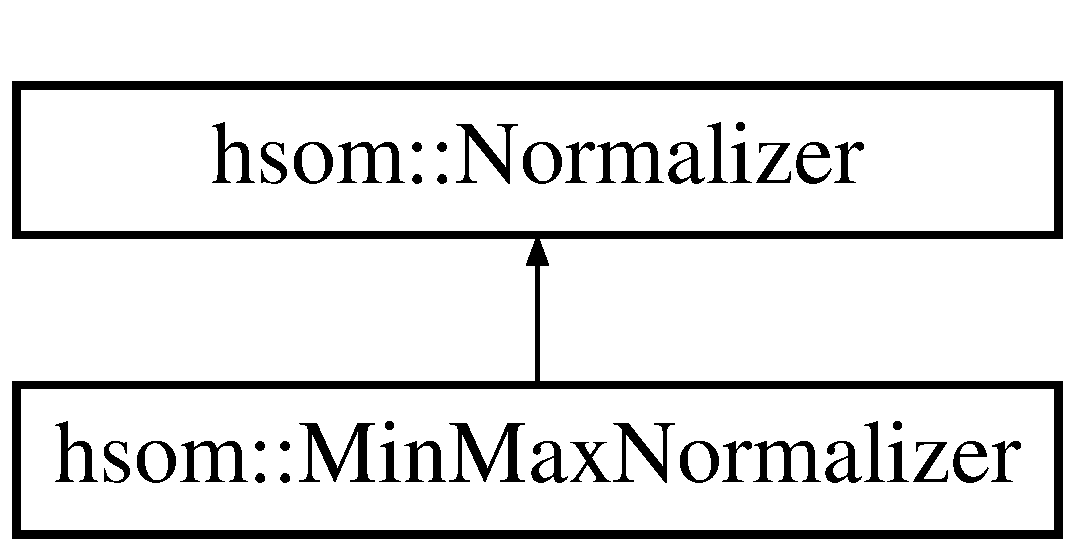
\includegraphics[height=2.000000cm]{classhsom_1_1_min_max_normalizer}
\end{center}
\end{figure}
\subsection*{\-Public \-Member \-Functions}
\begin{DoxyCompactItemize}
\item 
virtual void \hyperlink{classhsom_1_1_min_max_normalizer_a9d7504876aadfb2dc473af23550fef39}{normalize} (\hyperlink{classhsom_1_1_feature}{\-Feature} \&feature)
\item 
virtual void \hyperlink{classhsom_1_1_min_max_normalizer_a659a9e0299dee946934b37f2b62720fc}{set\-Feature} (\hyperlink{classhsom_1_1_feature}{\-Feature} \&feature)
\end{DoxyCompactItemize}
\subsection*{\-Protected \-Member \-Functions}
\begin{DoxyCompactItemize}
\item 
virtual void \hyperlink{classhsom_1_1_min_max_normalizer_a767b6a382aa190053e41f4c664f6594d}{calculate\-Normalizer} (\-Q\-Vector$<$ \-Feature\-Ptr $>$ features, \-Q\-Map$<$ \-Q\-String, \-Q\-Variant $>$ nomalizer\-Parameters)
\end{DoxyCompactItemize}


\subsection{\-Detailed \-Description}
\begin{DoxySeeAlso}{\-See also}
\hyperlink{normalizer_8h_source}{normalizer.\-h} for full documentation of the \hyperlink{classhsom_1_1_normalizer}{\-Normalizer} \-A\-P\-I 
\end{DoxySeeAlso}


\subsection{\-Member \-Function \-Documentation}
\hypertarget{classhsom_1_1_min_max_normalizer_a767b6a382aa190053e41f4c664f6594d}{\index{hsom\-::\-Min\-Max\-Normalizer@{hsom\-::\-Min\-Max\-Normalizer}!calculate\-Normalizer@{calculate\-Normalizer}}
\index{calculate\-Normalizer@{calculate\-Normalizer}!hsom::MinMaxNormalizer@{hsom\-::\-Min\-Max\-Normalizer}}
\subsubsection[{calculate\-Normalizer}]{\setlength{\rightskip}{0pt plus 5cm}void {\bf hsom\-::\-Min\-Max\-Normalizer\-::calculate\-Normalizer} (
\begin{DoxyParamCaption}
\item[{\-Q\-Vector$<$ \-Feature\-Ptr $>$}]{features, }
\item[{\-Q\-Map$<$ \-Q\-String, \-Q\-Variant $>$}]{nomalizer\-Parameters}
\end{DoxyParamCaption}
)\hspace{0.3cm}{\ttfamily  \mbox{[}protected, virtual\mbox{]}}}}\label{classhsom_1_1_min_max_normalizer_a767b6a382aa190053e41f4c664f6594d}
\begin{DoxySeeAlso}{\-See also}
\hyperlink{normalizer_8h_source}{normalizer.\-h} for full documentation 
\end{DoxySeeAlso}
\hypertarget{classhsom_1_1_min_max_normalizer_a9d7504876aadfb2dc473af23550fef39}{\index{hsom\-::\-Min\-Max\-Normalizer@{hsom\-::\-Min\-Max\-Normalizer}!normalize@{normalize}}
\index{normalize@{normalize}!hsom::MinMaxNormalizer@{hsom\-::\-Min\-Max\-Normalizer}}
\subsubsection[{normalize}]{\setlength{\rightskip}{0pt plus 5cm}void {\bf hsom\-::\-Min\-Max\-Normalizer\-::normalize} (
\begin{DoxyParamCaption}
\item[{{\bf \-Feature} \&}]{feature}
\end{DoxyParamCaption}
)\hspace{0.3cm}{\ttfamily  \mbox{[}virtual\mbox{]}}}}\label{classhsom_1_1_min_max_normalizer_a9d7504876aadfb2dc473af23550fef39}
\begin{DoxySeeAlso}{\-See also}
\hyperlink{normalizer_8h_source}{normalizer.\-h} for full documentation 
\end{DoxySeeAlso}


\-Implements \hyperlink{classhsom_1_1_normalizer_af00cb37e6079f3802b24389fb336debd}{hsom\-::\-Normalizer}.

\hypertarget{classhsom_1_1_min_max_normalizer_a659a9e0299dee946934b37f2b62720fc}{\index{hsom\-::\-Min\-Max\-Normalizer@{hsom\-::\-Min\-Max\-Normalizer}!set\-Feature@{set\-Feature}}
\index{set\-Feature@{set\-Feature}!hsom::MinMaxNormalizer@{hsom\-::\-Min\-Max\-Normalizer}}
\subsubsection[{set\-Feature}]{\setlength{\rightskip}{0pt plus 5cm}void {\bf hsom\-::\-Min\-Max\-Normalizer\-::set\-Feature} (
\begin{DoxyParamCaption}
\item[{{\bf \-Feature} \&}]{feature}
\end{DoxyParamCaption}
)\hspace{0.3cm}{\ttfamily  \mbox{[}virtual\mbox{]}}}}\label{classhsom_1_1_min_max_normalizer_a659a9e0299dee946934b37f2b62720fc}
\begin{DoxySeeAlso}{\-See also}
\hyperlink{normalizer_8h_source}{normalizer.\-h} for full documentation 
\end{DoxySeeAlso}


\-Implements \hyperlink{classhsom_1_1_normalizer_afb0c21572e09b44a67c49c4f18d34837}{hsom\-::\-Normalizer}.



\-The documentation for this class was generated from the following files\-:\begin{DoxyCompactItemize}
\item 
\-C\-:/\-Users/d3x874/\-Documents/source/urania/normalizers/minmaxnormalizer.\-h\item 
\-C\-:/\-Users/d3x874/\-Documents/source/urania/normalizers/minmaxnormalizer.\-cpp\end{DoxyCompactItemize}

\hypertarget{classhsom_1_1_normalizer}{\section{hsom\-:\-:\-Normalizer \-Class \-Reference}
\label{classhsom_1_1_normalizer}\index{hsom\-::\-Normalizer@{hsom\-::\-Normalizer}}
}


{\ttfamily \#include $<$normalizer.\-h$>$}

\-Inheritance diagram for hsom\-:\-:\-Normalizer\-:\begin{figure}[H]
\begin{center}
\leavevmode
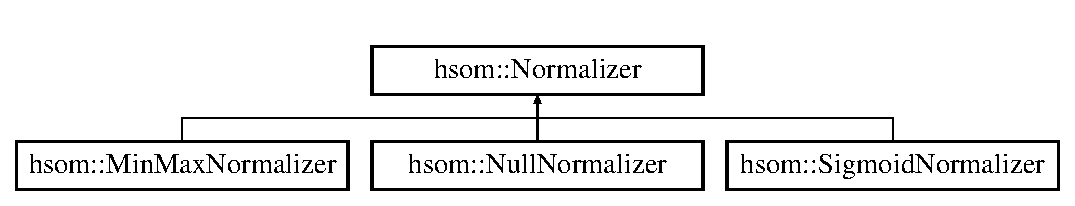
\includegraphics[height=2.000000cm]{classhsom_1_1_normalizer}
\end{center}
\end{figure}
\subsection*{\-Public \-Member \-Functions}
\begin{DoxyCompactItemize}
\item 
\hypertarget{classhsom_1_1_normalizer_a333d863efb0f68c743e85d6b0f2cda05}{\hyperlink{classhsom_1_1_normalizer_a333d863efb0f68c743e85d6b0f2cda05}{\-Normalizer} ()}\label{classhsom_1_1_normalizer_a333d863efb0f68c743e85d6b0f2cda05}

\begin{DoxyCompactList}\small\item\em \-Constructs a \hyperlink{classhsom_1_1_normalizer}{\-Normalizer}. \end{DoxyCompactList}\item 
void \hyperlink{classhsom_1_1_normalizer_ad033162f2f4d207c170fd97e349dfb65}{calculate} (\-Q\-Vector$<$ \hyperlink{classhsom_1_1_feature}{\-Feature} $>$ features, \-Q\-Map$<$ \-Q\-String, \-Q\-Variant $>$ nomalizer\-Parameters)
\begin{DoxyCompactList}\small\item\em \-Computes the normalization statisticts to be used for future normalizations. \end{DoxyCompactList}\item 
\hypertarget{classhsom_1_1_normalizer_ada54af29a7b7527eb555d267ca82d849}{virtual void \hyperlink{classhsom_1_1_normalizer_ada54af29a7b7527eb555d267ca82d849}{clear} ()=0}\label{classhsom_1_1_normalizer_ada54af29a7b7527eb555d267ca82d849}

\begin{DoxyCompactList}\small\item\em \-Clears the normalizer. \end{DoxyCompactList}\item 
\hypertarget{classhsom_1_1_normalizer_af00cb37e6079f3802b24389fb336debd}{virtual void \hyperlink{classhsom_1_1_normalizer_af00cb37e6079f3802b24389fb336debd}{normalize} (\hyperlink{classhsom_1_1_feature}{\-Feature} \&feature)=0}\label{classhsom_1_1_normalizer_af00cb37e6079f3802b24389fb336debd}

\begin{DoxyCompactList}\small\item\em \-Normalizes a single feature. \end{DoxyCompactList}\item 
\hypertarget{classhsom_1_1_normalizer_afb0c21572e09b44a67c49c4f18d34837}{virtual void \hyperlink{classhsom_1_1_normalizer_afb0c21572e09b44a67c49c4f18d34837}{set\-Feature} (\hyperlink{classhsom_1_1_feature}{\-Feature} \&feature)=0}\label{classhsom_1_1_normalizer_afb0c21572e09b44a67c49c4f18d34837}

\begin{DoxyCompactList}\small\item\em \-Sets a features values based upon calculated normalization. \end{DoxyCompactList}\end{DoxyCompactItemize}
\subsection*{\-Protected \-Member \-Functions}
\begin{DoxyCompactItemize}
\item 
virtual void \hyperlink{classhsom_1_1_normalizer_addd6ca248cc630ffa677788872b0ee13}{calculate\-Normalizer} (\-Q\-Vector$<$ \hyperlink{classhsom_1_1_feature}{\-Feature} $>$ features, \-Q\-Map$<$ \-Q\-String, \-Q\-Variant $>$ nomalizer\-Parameters)=0
\begin{DoxyCompactList}\small\item\em \-Computes the normalization statisticts to be used for future normalizations. \end{DoxyCompactList}\end{DoxyCompactItemize}
\subsection*{\-Protected \-Attributes}
\begin{DoxyCompactItemize}
\item 
\hypertarget{classhsom_1_1_normalizer_a0f156a4d8557dd56026ba1a82eefed23}{\-Q\-Map$<$ \-Q\-String, \-Q\-Variant $>$ \hyperlink{classhsom_1_1_normalizer_a0f156a4d8557dd56026ba1a82eefed23}{\-\_\-calculation\-Parameters}}\label{classhsom_1_1_normalizer_a0f156a4d8557dd56026ba1a82eefed23}

\begin{DoxyCompactList}\small\item\em \-Describes the parameters used to tune the calculation of this normalizer. \end{DoxyCompactList}\item 
\hypertarget{classhsom_1_1_normalizer_a3c888c25a91e9e01755c284b1100bdb3}{\-Rand\-Master \hyperlink{classhsom_1_1_normalizer_a3c888c25a91e9e01755c284b1100bdb3}{randomizer}}\label{classhsom_1_1_normalizer_a3c888c25a91e9e01755c284b1100bdb3}

\begin{DoxyCompactList}\small\item\em \-Provides random functionality if needed by derived instances. \end{DoxyCompactList}\end{DoxyCompactItemize}


\subsection{\-Detailed \-Description}
\begin{DoxyRefDesc}{\-Todo}
\item[\hyperlink{todo__todo000015}{\-Todo}]\-Document \-Classes and files \end{DoxyRefDesc}


\subsection{\-Member \-Function \-Documentation}
\hypertarget{classhsom_1_1_normalizer_ad033162f2f4d207c170fd97e349dfb65}{\index{hsom\-::\-Normalizer@{hsom\-::\-Normalizer}!calculate@{calculate}}
\index{calculate@{calculate}!hsom::Normalizer@{hsom\-::\-Normalizer}}
\subsubsection[{calculate}]{\setlength{\rightskip}{0pt plus 5cm}void {\bf hsom\-::\-Normalizer\-::calculate} (
\begin{DoxyParamCaption}
\item[{\-Q\-Vector$<$ {\bf \-Feature} $>$}]{features, }
\item[{\-Q\-Map$<$ \-Q\-String, \-Q\-Variant $>$}]{nomalizer\-Parameters}
\end{DoxyParamCaption}
)}}\label{classhsom_1_1_normalizer_ad033162f2f4d207c170fd97e349dfb65}


\-Computes the normalization statisticts to be used for future normalizations. 

\begin{DoxyNote}{\-Note}
\-This function calls the virtual calculate\-Normalizer function. \-The calculate\-Normalizer function should never be called explicitly. 
\end{DoxyNote}

\begin{DoxyParams}{\-Parameters}
{\em features} & \-A sample of features for which to compute the normalization \\
\hline
{\em nomalizer\-Parameters} & \-The tuning parameters used to compute the normalization \\
\hline
\end{DoxyParams}
\hypertarget{classhsom_1_1_normalizer_addd6ca248cc630ffa677788872b0ee13}{\index{hsom\-::\-Normalizer@{hsom\-::\-Normalizer}!calculate\-Normalizer@{calculate\-Normalizer}}
\index{calculate\-Normalizer@{calculate\-Normalizer}!hsom::Normalizer@{hsom\-::\-Normalizer}}
\subsubsection[{calculate\-Normalizer}]{\setlength{\rightskip}{0pt plus 5cm}virtual void {\bf hsom\-::\-Normalizer\-::calculate\-Normalizer} (
\begin{DoxyParamCaption}
\item[{\-Q\-Vector$<$ {\bf \-Feature} $>$}]{features, }
\item[{\-Q\-Map$<$ \-Q\-String, \-Q\-Variant $>$}]{nomalizer\-Parameters}
\end{DoxyParamCaption}
)\hspace{0.3cm}{\ttfamily  \mbox{[}protected, pure virtual\mbox{]}}}}\label{classhsom_1_1_normalizer_addd6ca248cc630ffa677788872b0ee13}


\-Computes the normalization statisticts to be used for future normalizations. 

\begin{DoxyNote}{\-Note}
\-This function is called by \hyperlink{classhsom_1_1_normalizer_ad033162f2f4d207c170fd97e349dfb65}{calculate()} in this base class. \-It should never be called explicitly. 
\end{DoxyNote}

\begin{DoxyParams}{\-Parameters}
{\em features} & \-A sample of features for which to compute the normalization \\
\hline
{\em nomalizer\-Parameters} & \-The tuning parameters used to compute the normalization \\
\hline
\end{DoxyParams}


\-Implemented in \hyperlink{classhsom_1_1_sigmoid_normalizer_a96240b51c8c107cbb1183b6f61cd5a8a}{hsom\-::\-Sigmoid\-Normalizer}, and \hyperlink{classhsom_1_1_null_normalizer_afa74034fd30d11ee08535078adabb190}{hsom\-::\-Null\-Normalizer}.



\-The documentation for this class was generated from the following files\-:\begin{DoxyCompactItemize}
\item 
\-C\-:/\-Users/d3x874/\-Documents/source/urania/normalizers/normalizer.\-h\item 
\-C\-:/\-Users/d3x874/\-Documents/source/urania/normalizers/normalizer.\-cpp\end{DoxyCompactItemize}

\hypertarget{classhsom_1_1_null_normalizer}{\section{hsom\-:\-:\-Null\-Normalizer \-Class \-Reference}
\label{classhsom_1_1_null_normalizer}\index{hsom\-::\-Null\-Normalizer@{hsom\-::\-Null\-Normalizer}}
}


{\ttfamily \#include $<$nullnormalizer.\-h$>$}

\-Inheritance diagram for hsom\-:\-:\-Null\-Normalizer\-:\begin{figure}[H]
\begin{center}
\leavevmode
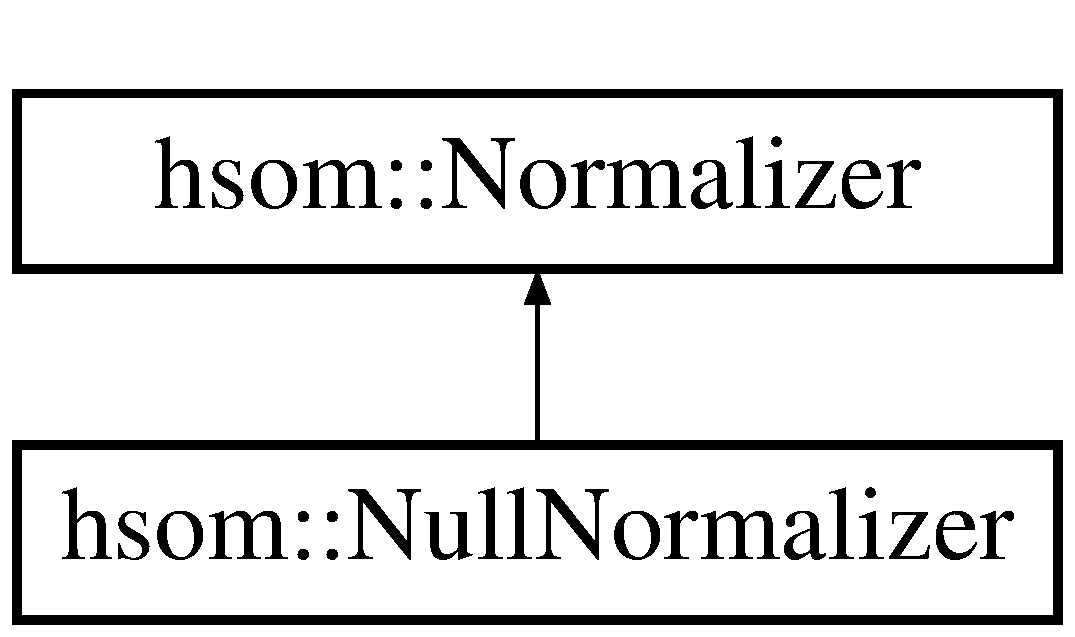
\includegraphics[height=2.000000cm]{classhsom_1_1_null_normalizer}
\end{center}
\end{figure}
\subsection*{\-Public \-Member \-Functions}
\begin{DoxyCompactItemize}
\item 
virtual void \hyperlink{classhsom_1_1_null_normalizer_a53a02e902af518f06611bf8d787f4832}{normalize} (\hyperlink{classhsom_1_1_feature}{\-Feature} \&)
\item 
virtual void \hyperlink{classhsom_1_1_null_normalizer_aace8f0e20fa4592ad7557a6485361239}{set\-Feature} (\hyperlink{classhsom_1_1_feature}{\-Feature} \&feature)
\end{DoxyCompactItemize}
\subsection*{\-Protected \-Member \-Functions}
\begin{DoxyCompactItemize}
\item 
virtual void \hyperlink{classhsom_1_1_null_normalizer_afa74034fd30d11ee08535078adabb190}{calculate\-Normalizer} (\-Q\-Vector$<$ \hyperlink{classhsom_1_1_feature}{\-Feature} $>$, \-Q\-Map$<$ \-Q\-String, \-Q\-Variant $>$)
\end{DoxyCompactItemize}


\subsection{\-Detailed \-Description}
\begin{DoxySeeAlso}{\-See also}
\hyperlink{normalizer_8h_source}{normalizer.\-h} for full documentation of the \hyperlink{classhsom_1_1_normalizer}{\-Normalizer} \-A\-P\-I 
\end{DoxySeeAlso}


\subsection{\-Member \-Function \-Documentation}
\hypertarget{classhsom_1_1_null_normalizer_afa74034fd30d11ee08535078adabb190}{\index{hsom\-::\-Null\-Normalizer@{hsom\-::\-Null\-Normalizer}!calculate\-Normalizer@{calculate\-Normalizer}}
\index{calculate\-Normalizer@{calculate\-Normalizer}!hsom::NullNormalizer@{hsom\-::\-Null\-Normalizer}}
\subsubsection[{calculate\-Normalizer}]{\setlength{\rightskip}{0pt plus 5cm}void {\bf hsom\-::\-Null\-Normalizer\-::calculate\-Normalizer} (
\begin{DoxyParamCaption}
\item[{\-Q\-Vector$<$ {\bf \-Feature} $>$}]{, }
\item[{\-Q\-Map$<$ \-Q\-String, \-Q\-Variant $>$}]{}
\end{DoxyParamCaption}
)\hspace{0.3cm}{\ttfamily  \mbox{[}protected, virtual\mbox{]}}}}\label{classhsom_1_1_null_normalizer_afa74034fd30d11ee08535078adabb190}
\begin{DoxySeeAlso}{\-See also}
\hyperlink{normalizer_8h_source}{normalizer.\-h} for full documentation 
\end{DoxySeeAlso}


\-Implements \hyperlink{classhsom_1_1_normalizer_addd6ca248cc630ffa677788872b0ee13}{hsom\-::\-Normalizer}.

\hypertarget{classhsom_1_1_null_normalizer_a53a02e902af518f06611bf8d787f4832}{\index{hsom\-::\-Null\-Normalizer@{hsom\-::\-Null\-Normalizer}!normalize@{normalize}}
\index{normalize@{normalize}!hsom::NullNormalizer@{hsom\-::\-Null\-Normalizer}}
\subsubsection[{normalize}]{\setlength{\rightskip}{0pt plus 5cm}void {\bf hsom\-::\-Null\-Normalizer\-::normalize} (
\begin{DoxyParamCaption}
\item[{{\bf \-Feature} \&}]{}
\end{DoxyParamCaption}
)\hspace{0.3cm}{\ttfamily  \mbox{[}virtual\mbox{]}}}}\label{classhsom_1_1_null_normalizer_a53a02e902af518f06611bf8d787f4832}
\begin{DoxySeeAlso}{\-See also}
\hyperlink{normalizer_8h_source}{normalizer.\-h} for full documentation 
\end{DoxySeeAlso}


\-Implements \hyperlink{classhsom_1_1_normalizer_af00cb37e6079f3802b24389fb336debd}{hsom\-::\-Normalizer}.

\hypertarget{classhsom_1_1_null_normalizer_aace8f0e20fa4592ad7557a6485361239}{\index{hsom\-::\-Null\-Normalizer@{hsom\-::\-Null\-Normalizer}!set\-Feature@{set\-Feature}}
\index{set\-Feature@{set\-Feature}!hsom::NullNormalizer@{hsom\-::\-Null\-Normalizer}}
\subsubsection[{set\-Feature}]{\setlength{\rightskip}{0pt plus 5cm}void {\bf hsom\-::\-Null\-Normalizer\-::set\-Feature} (
\begin{DoxyParamCaption}
\item[{{\bf \-Feature} \&}]{feature}
\end{DoxyParamCaption}
)\hspace{0.3cm}{\ttfamily  \mbox{[}virtual\mbox{]}}}}\label{classhsom_1_1_null_normalizer_aace8f0e20fa4592ad7557a6485361239}
\begin{DoxySeeAlso}{\-See also}
\hyperlink{normalizer_8h_source}{normalizer.\-h} for full documentation 
\end{DoxySeeAlso}


\-Implements \hyperlink{classhsom_1_1_normalizer_afb0c21572e09b44a67c49c4f18d34837}{hsom\-::\-Normalizer}.



\-The documentation for this class was generated from the following files\-:\begin{DoxyCompactItemize}
\item 
\-C\-:/\-Users/d3x874/\-Documents/source/urania/normalizers/nullnormalizer.\-h\item 
\-C\-:/\-Users/d3x874/\-Documents/source/urania/normalizers/nullnormalizer.\-cpp\end{DoxyCompactItemize}

\hypertarget{classhsom_1_1_quad_grid}{\section{hsom\-:\-:\-Quad\-Grid$<$ \-T $>$ \-Class \-Template \-Reference}
\label{classhsom_1_1_quad_grid}\index{hsom\-::\-Quad\-Grid$<$ T $>$@{hsom\-::\-Quad\-Grid$<$ T $>$}}
}


{\ttfamily \#include $<$quadgrid.\-hpp$>$}

\-Inheritance diagram for hsom\-:\-:\-Quad\-Grid$<$ \-T $>$\-:\begin{figure}[H]
\begin{center}
\leavevmode
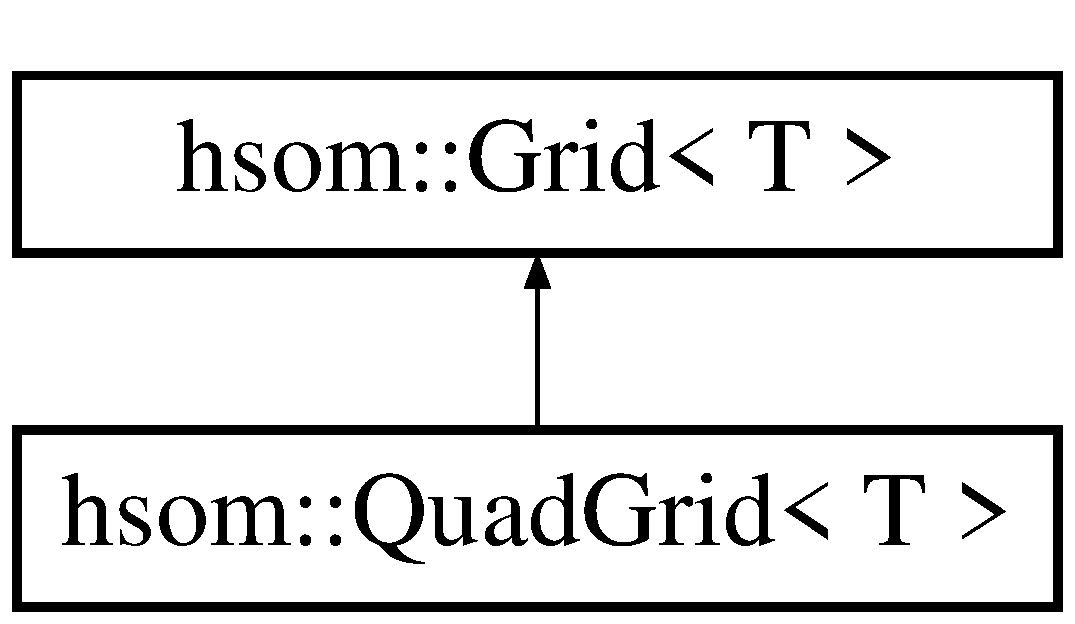
\includegraphics[height=2.000000cm]{classhsom_1_1_quad_grid}
\end{center}
\end{figure}
\subsection*{\-Public \-Member \-Functions}
\begin{DoxyCompactItemize}
\item 
\hypertarget{classhsom_1_1_quad_grid_a6b20b45657281184ac54ed0bda4ad088}{\hyperlink{classhsom_1_1_quad_grid_a6b20b45657281184ac54ed0bda4ad088}{\-Quad\-Grid} ()}\label{classhsom_1_1_quad_grid_a6b20b45657281184ac54ed0bda4ad088}

\begin{DoxyCompactList}\small\item\em \-Constructs a hex grid with no size information. \end{DoxyCompactList}\item 
\hyperlink{classhsom_1_1_quad_grid_a0cec637e161240b9a7241ac83d0c6ff4}{\-Quad\-Grid} (\-Q\-Vector$<$ int $>$ \hyperlink{classhsom_1_1_grid_a3e846473299eb2c7c259659eb61a6234}{size})
\begin{DoxyCompactList}\small\item\em \-Constructs the hex grid with a specified size. \end{DoxyCompactList}\item 
\hyperlink{classhsom_1_1_quad_grid_a3aebaea9b496991fdd61026e74d013d4}{\-Quad\-Grid} (int w, int h)
\begin{DoxyCompactList}\small\item\em \-Constructs the hex grid with a specified size. \end{DoxyCompactList}\item 
\hyperlink{classhsom_1_1_quad_grid_abe9c6802339cc0fe89574c718b16cefc}{\-Quad\-Grid} (\-Q\-Vector$<$ int $>$ \hyperlink{classhsom_1_1_grid_a3e846473299eb2c7c259659eb61a6234}{size}, \-Q\-Vector$<$ \-T $>$ \hyperlink{classhsom_1_1_grid_ae6b6ffb72e86c3904e8ac21253d85a24}{items})
\begin{DoxyCompactList}\small\item\em \-Constructs the hex grid with the specified size and fills it with the supplied values. \end{DoxyCompactList}\item 
\hyperlink{classhsom_1_1_quad_grid_ab9762ecd6652451e4243bfa55d762b45}{\-Quad\-Grid} (int w, int h, \-Q\-Vector$<$ \-T $>$ \hyperlink{classhsom_1_1_grid_ae6b6ffb72e86c3904e8ac21253d85a24}{items})
\begin{DoxyCompactList}\small\item\em \-Constructs the hex grid with the specified size and fills it with the supplied values. \end{DoxyCompactList}\item 
\hypertarget{classhsom_1_1_quad_grid_abe87f9710cfe2e66b90243598928b1c0}{virtual \hyperlink{classhsom_1_1_quad_grid_abe87f9710cfe2e66b90243598928b1c0}{$\sim$\-Quad\-Grid} ()}\label{classhsom_1_1_quad_grid_abe87f9710cfe2e66b90243598928b1c0}

\begin{DoxyCompactList}\small\item\em \-Destructs the \hyperlink{classhsom_1_1_hex_grid}{\-Hex\-Grid}. \end{DoxyCompactList}\item 
\hypertarget{classhsom_1_1_quad_grid_a0cdfb7f9c5ce4e36510279f1edf8133b}{int {\bfseries w} ()}\label{classhsom_1_1_quad_grid_a0cdfb7f9c5ce4e36510279f1edf8133b}

\item 
\hypertarget{classhsom_1_1_quad_grid_afe8556629d71bd960710ba566b245c9a}{int {\bfseries h} ()}\label{classhsom_1_1_quad_grid_afe8556629d71bd960710ba566b245c9a}

\item 
\hypertarget{classhsom_1_1_quad_grid_a249f85b1d84a4219ccdd1d42d6a283f3}{virtual void \hyperlink{classhsom_1_1_quad_grid_a249f85b1d84a4219ccdd1d42d6a283f3}{check\-Size} (\-Q\-Vector$<$ int $>$ \hyperlink{classhsom_1_1_grid_a3e846473299eb2c7c259659eb61a6234}{size})}\label{classhsom_1_1_quad_grid_a249f85b1d84a4219ccdd1d42d6a283f3}

\begin{DoxyCompactList}\small\item\em \-Checks the supplied size to ensure that it is valid for the \hyperlink{classhsom_1_1_hex_grid}{\-Hex\-Grid}. \end{DoxyCompactList}\item 
\hypertarget{classhsom_1_1_quad_grid_a426dfe4e7a75f55c01d9e99865941633}{virtual int \hyperlink{classhsom_1_1_quad_grid_a426dfe4e7a75f55c01d9e99865941633}{capacity\-From\-Size} (\-Q\-Vector$<$ int $>$ \hyperlink{classhsom_1_1_grid_a3e846473299eb2c7c259659eb61a6234}{size})}\label{classhsom_1_1_quad_grid_a426dfe4e7a75f55c01d9e99865941633}

\begin{DoxyCompactList}\small\item\em \-Gets the capacity of a grid based on the size of the grid. \end{DoxyCompactList}\item 
\hypertarget{classhsom_1_1_quad_grid_a73f94c48b7544917753883ccd813c9e6}{virtual void \hyperlink{classhsom_1_1_quad_grid_a73f94c48b7544917753883ccd813c9e6}{check\-Coords} (\-Q\-Vector$<$ int $>$ \hyperlink{classhsom_1_1_quad_grid_a8f91269433c403a6034efdec7e97104b}{coords})}\label{classhsom_1_1_quad_grid_a73f94c48b7544917753883ccd813c9e6}

\begin{DoxyCompactList}\small\item\em \-Checks a given point to ensure it is a valid reference to an element in the grid. \end{DoxyCompactList}\item 
virtual int \hyperlink{classhsom_1_1_quad_grid_a5623e24a82df043cec092e5cb61aed34}{index} (\-Q\-Vector$<$ int $>$ \hyperlink{classhsom_1_1_quad_grid_a8f91269433c403a6034efdec7e97104b}{coords})
\begin{DoxyCompactList}\small\item\em \-Fetches the index for the slot at the specified coordinates. \end{DoxyCompactList}\item 
virtual \-Q\-Vector$<$ int $>$ \hyperlink{classhsom_1_1_quad_grid_a8f91269433c403a6034efdec7e97104b}{coords} (int idx)
\begin{DoxyCompactList}\small\item\em \-Fetches the coordinates given an index. \end{DoxyCompactList}\item 
\hypertarget{classhsom_1_1_quad_grid_ae78eac9f185cb53602023827f6060773}{virtual \-Q\-Vector$<$ double $>$ \hyperlink{classhsom_1_1_quad_grid_ae78eac9f185cb53602023827f6060773}{real\-Bounds} ()}\label{classhsom_1_1_quad_grid_ae78eac9f185cb53602023827f6060773}

\begin{DoxyCompactList}\small\item\em \-Fetches the extents of the real coordinate mapping space ( should only be used for visualization ) \end{DoxyCompactList}\item 
\hypertarget{classhsom_1_1_quad_grid_aa5a1d2ccf49fe787a0bb433274f1c6fd}{virtual \-Q\-Vector$<$ double $>$ \hyperlink{classhsom_1_1_quad_grid_aa5a1d2ccf49fe787a0bb433274f1c6fd}{real\-Coords} (int idx)}\label{classhsom_1_1_quad_grid_aa5a1d2ccf49fe787a0bb433274f1c6fd}

\begin{DoxyCompactList}\small\item\em \-Fetches the real coordinates of a given index in the grid ( should only be used for visualization ) \end{DoxyCompactList}\item 
virtual int \hyperlink{classhsom_1_1_quad_grid_a8f5bc5583e2d254f3850dfa0542a5505}{diagonal} ()
\begin{DoxyCompactList}\small\item\em \-Fetches the length of the major diagonal running through the grid. \end{DoxyCompactList}\item 
\hypertarget{classhsom_1_1_quad_grid_a28fe768065b4559a5e9e0e7c9fcca1c8}{virtual int \hyperlink{classhsom_1_1_quad_grid_a28fe768065b4559a5e9e0e7c9fcca1c8}{distance} (int idx0, int idx1)}\label{classhsom_1_1_quad_grid_a28fe768065b4559a5e9e0e7c9fcca1c8}

\begin{DoxyCompactList}\small\item\em \-Fetches indices for all slots within a radius of the specified slot. \end{DoxyCompactList}\end{DoxyCompactItemize}


\subsection{\-Detailed \-Description}
\subsubsection*{template$<$class T$>$class hsom\-::\-Quad\-Grid$<$ T $>$}

\-The \hyperlink{classhsom_1_1_hex_grid}{\-Hex\-Grid} class provides the basis for the spatial organization of the \-Self \-Organizing \-Map. \-It provides a hexagonal grid which supports neighborhood searches, edge wrapping, and other functionality. 

\subsection{\-Constructor \& \-Destructor \-Documentation}
\hypertarget{classhsom_1_1_quad_grid_a0cec637e161240b9a7241ac83d0c6ff4}{\index{hsom\-::\-Quad\-Grid@{hsom\-::\-Quad\-Grid}!\-Quad\-Grid@{\-Quad\-Grid}}
\index{\-Quad\-Grid@{\-Quad\-Grid}!hsom::QuadGrid@{hsom\-::\-Quad\-Grid}}
\subsubsection[{\-Quad\-Grid}]{\setlength{\rightskip}{0pt plus 5cm}template$<$class T $>$ {\bf hsom\-::\-Quad\-Grid}$<$ \-T $>$\-::{\bf \-Quad\-Grid} (
\begin{DoxyParamCaption}
\item[{\-Q\-Vector$<$ int $>$}]{size}
\end{DoxyParamCaption}
)\hspace{0.3cm}{\ttfamily  \mbox{[}inline\mbox{]}}}}\label{classhsom_1_1_quad_grid_a0cec637e161240b9a7241ac83d0c6ff4}


\-Constructs the hex grid with a specified size. 


\begin{DoxyParams}{\-Parameters}
{\em size} & \-The size of the new grid \\
\hline
\end{DoxyParams}
\hypertarget{classhsom_1_1_quad_grid_a3aebaea9b496991fdd61026e74d013d4}{\index{hsom\-::\-Quad\-Grid@{hsom\-::\-Quad\-Grid}!\-Quad\-Grid@{\-Quad\-Grid}}
\index{\-Quad\-Grid@{\-Quad\-Grid}!hsom::QuadGrid@{hsom\-::\-Quad\-Grid}}
\subsubsection[{\-Quad\-Grid}]{\setlength{\rightskip}{0pt plus 5cm}template$<$class T $>$ {\bf hsom\-::\-Quad\-Grid}$<$ \-T $>$\-::{\bf \-Quad\-Grid} (
\begin{DoxyParamCaption}
\item[{int}]{w, }
\item[{int}]{h}
\end{DoxyParamCaption}
)\hspace{0.3cm}{\ttfamily  \mbox{[}inline\mbox{]}}}}\label{classhsom_1_1_quad_grid_a3aebaea9b496991fdd61026e74d013d4}


\-Constructs the hex grid with a specified size. 


\begin{DoxyParams}{\-Parameters}
{\em w} & \-The width of the hex grid \\
\hline
{\em h} & \-The height of the hex grid \\
\hline
\end{DoxyParams}
\hypertarget{classhsom_1_1_quad_grid_abe9c6802339cc0fe89574c718b16cefc}{\index{hsom\-::\-Quad\-Grid@{hsom\-::\-Quad\-Grid}!\-Quad\-Grid@{\-Quad\-Grid}}
\index{\-Quad\-Grid@{\-Quad\-Grid}!hsom::QuadGrid@{hsom\-::\-Quad\-Grid}}
\subsubsection[{\-Quad\-Grid}]{\setlength{\rightskip}{0pt plus 5cm}template$<$class T $>$ {\bf hsom\-::\-Quad\-Grid}$<$ \-T $>$\-::{\bf \-Quad\-Grid} (
\begin{DoxyParamCaption}
\item[{\-Q\-Vector$<$ int $>$}]{size, }
\item[{\-Q\-Vector$<$ \-T $>$}]{items}
\end{DoxyParamCaption}
)\hspace{0.3cm}{\ttfamily  \mbox{[}inline\mbox{]}}}}\label{classhsom_1_1_quad_grid_abe9c6802339cc0fe89574c718b16cefc}


\-Constructs the hex grid with the specified size and fills it with the supplied values. 


\begin{DoxyParams}{\-Parameters}
{\em size} & \-The size of the new grid \\
\hline
{\em items} & \-The items with which to populate the grid \\
\hline
\end{DoxyParams}
\hypertarget{classhsom_1_1_quad_grid_ab9762ecd6652451e4243bfa55d762b45}{\index{hsom\-::\-Quad\-Grid@{hsom\-::\-Quad\-Grid}!\-Quad\-Grid@{\-Quad\-Grid}}
\index{\-Quad\-Grid@{\-Quad\-Grid}!hsom::QuadGrid@{hsom\-::\-Quad\-Grid}}
\subsubsection[{\-Quad\-Grid}]{\setlength{\rightskip}{0pt plus 5cm}template$<$class T $>$ {\bf hsom\-::\-Quad\-Grid}$<$ \-T $>$\-::{\bf \-Quad\-Grid} (
\begin{DoxyParamCaption}
\item[{int}]{w, }
\item[{int}]{h, }
\item[{\-Q\-Vector$<$ \-T $>$}]{items}
\end{DoxyParamCaption}
)\hspace{0.3cm}{\ttfamily  \mbox{[}inline\mbox{]}}}}\label{classhsom_1_1_quad_grid_ab9762ecd6652451e4243bfa55d762b45}


\-Constructs the hex grid with the specified size and fills it with the supplied values. 


\begin{DoxyParams}{\-Parameters}
{\em w} & \-The width of the hex grid \\
\hline
{\em h} & \-The height of the hex grid \\
\hline
{\em items} & \-The items with which to populate the grid \\
\hline
\end{DoxyParams}


\subsection{\-Member \-Function \-Documentation}
\hypertarget{classhsom_1_1_quad_grid_a8f91269433c403a6034efdec7e97104b}{\index{hsom\-::\-Quad\-Grid@{hsom\-::\-Quad\-Grid}!coords@{coords}}
\index{coords@{coords}!hsom::QuadGrid@{hsom\-::\-Quad\-Grid}}
\subsubsection[{coords}]{\setlength{\rightskip}{0pt plus 5cm}template$<$class T $>$ virtual \-Q\-Vector$<$int$>$ {\bf hsom\-::\-Quad\-Grid}$<$ \-T $>$\-::{\bf coords} (
\begin{DoxyParamCaption}
\item[{int}]{idx}
\end{DoxyParamCaption}
)\hspace{0.3cm}{\ttfamily  \mbox{[}inline, virtual\mbox{]}}}}\label{classhsom_1_1_quad_grid_a8f91269433c403a6034efdec7e97104b}


\-Fetches the coordinates given an index. 


\begin{DoxyParams}{\-Parameters}
{\em idx} & \-The index in the grid for which to fetch the coordinates \\
\hline
\end{DoxyParams}


\-Implements \hyperlink{classhsom_1_1_grid_a4a68c15ff3ffcd052bff769e4d9e899b}{hsom\-::\-Grid$<$ T $>$}.

\hypertarget{classhsom_1_1_quad_grid_a8f5bc5583e2d254f3850dfa0542a5505}{\index{hsom\-::\-Quad\-Grid@{hsom\-::\-Quad\-Grid}!diagonal@{diagonal}}
\index{diagonal@{diagonal}!hsom::QuadGrid@{hsom\-::\-Quad\-Grid}}
\subsubsection[{diagonal}]{\setlength{\rightskip}{0pt plus 5cm}template$<$class T $>$ virtual int {\bf hsom\-::\-Quad\-Grid}$<$ \-T $>$\-::{\bf diagonal} (
\begin{DoxyParamCaption}
{}
\end{DoxyParamCaption}
)\hspace{0.3cm}{\ttfamily  \mbox{[}inline, virtual\mbox{]}}}}\label{classhsom_1_1_quad_grid_a8f5bc5583e2d254f3850dfa0542a5505}


\-Fetches the length of the major diagonal running through the grid. 

\begin{DoxyRefDesc}{\-Todo}
\item[\hyperlink{todo__todo000009}{\-Todo}]\-Come up with a more precise computation of this \end{DoxyRefDesc}


\-Implements \hyperlink{classhsom_1_1_grid_acc0364a698525d1239a7042eb01f79e6}{hsom\-::\-Grid$<$ T $>$}.

\hypertarget{classhsom_1_1_quad_grid_a5623e24a82df043cec092e5cb61aed34}{\index{hsom\-::\-Quad\-Grid@{hsom\-::\-Quad\-Grid}!index@{index}}
\index{index@{index}!hsom::QuadGrid@{hsom\-::\-Quad\-Grid}}
\subsubsection[{index}]{\setlength{\rightskip}{0pt plus 5cm}template$<$class T $>$ virtual int {\bf hsom\-::\-Quad\-Grid}$<$ \-T $>$\-::{\bf index} (
\begin{DoxyParamCaption}
\item[{\-Q\-Vector$<$ int $>$}]{coords}
\end{DoxyParamCaption}
)\hspace{0.3cm}{\ttfamily  \mbox{[}inline, virtual\mbox{]}}}}\label{classhsom_1_1_quad_grid_a5623e24a82df043cec092e5cb61aed34}


\-Fetches the index for the slot at the specified coordinates. 


\begin{DoxyParams}{\-Parameters}
{\em coords} & \-The point in the grid for which to fetch the index \\
\hline
\end{DoxyParams}


\-Implements \hyperlink{classhsom_1_1_grid_a1c3162ea843ab3f7e79136425e011a5d}{hsom\-::\-Grid$<$ T $>$}.



\-The documentation for this class was generated from the following file\-:\begin{DoxyCompactItemize}
\item 
\-C\-:/\-Users/d3x874/\-Documents/source/urania/grids/quadgrid.\-hpp\end{DoxyCompactItemize}

\hypertarget{classhsom_1_1_sigmoid_normalizer}{\section{hsom\-:\-:\-Sigmoid\-Normalizer \-Class \-Reference}
\label{classhsom_1_1_sigmoid_normalizer}\index{hsom\-::\-Sigmoid\-Normalizer@{hsom\-::\-Sigmoid\-Normalizer}}
}


{\ttfamily \#include $<$sigmoidnormalizer.\-h$>$}

\-Inheritance diagram for hsom\-:\-:\-Sigmoid\-Normalizer\-:\begin{figure}[H]
\begin{center}
\leavevmode
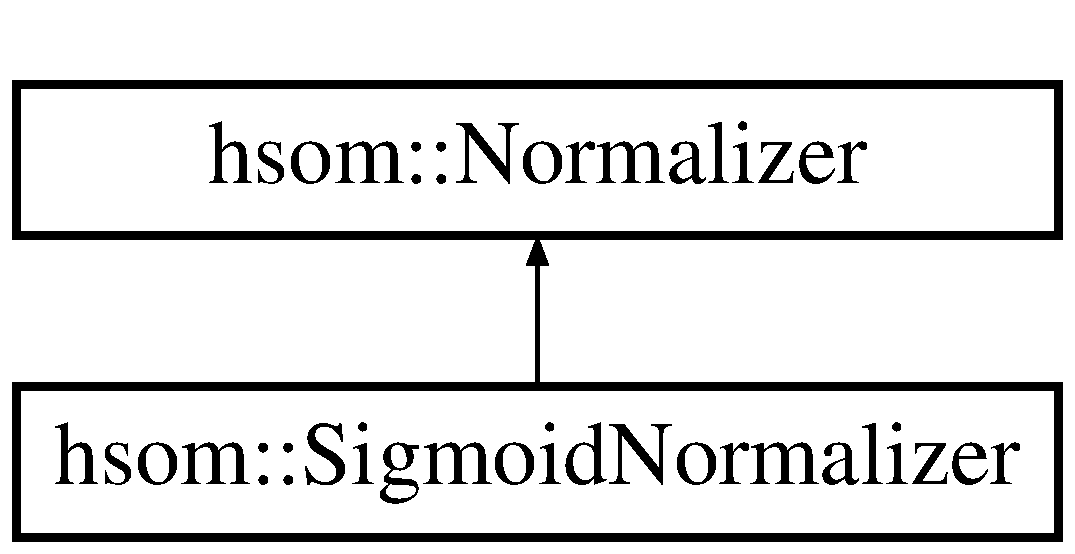
\includegraphics[height=2.000000cm]{classhsom_1_1_sigmoid_normalizer}
\end{center}
\end{figure}
\subsection*{\-Public \-Member \-Functions}
\begin{DoxyCompactItemize}
\item 
virtual void \hyperlink{classhsom_1_1_sigmoid_normalizer_a16256f0977a0bb6983e4e46edf00067b}{normalize} (\hyperlink{classhsom_1_1_feature}{\-Feature} \&feature)
\item 
virtual void \hyperlink{classhsom_1_1_sigmoid_normalizer_af31b9bcbcfefd2c98881a92116c0ba2c}{set\-Feature} (\hyperlink{classhsom_1_1_feature}{\-Feature} \&feature)
\end{DoxyCompactItemize}
\subsection*{\-Protected \-Member \-Functions}
\begin{DoxyCompactItemize}
\item 
virtual void \hyperlink{classhsom_1_1_sigmoid_normalizer_a96240b51c8c107cbb1183b6f61cd5a8a}{calculate\-Normalizer} (\-Q\-Vector$<$ \hyperlink{classhsom_1_1_feature}{\-Feature} $>$ features, \-Q\-Map$<$ \-Q\-String, \-Q\-Variant $>$ normalizer\-Parameters)
\end{DoxyCompactItemize}


\subsection{\-Detailed \-Description}
\begin{DoxySeeAlso}{\-See also}
\hyperlink{normalizer_8h_source}{normalizer.\-h} for full documentation of the \hyperlink{classhsom_1_1_normalizer}{\-Normalizer} \-A\-P\-I 
\end{DoxySeeAlso}


\subsection{\-Member \-Function \-Documentation}
\hypertarget{classhsom_1_1_sigmoid_normalizer_a96240b51c8c107cbb1183b6f61cd5a8a}{\index{hsom\-::\-Sigmoid\-Normalizer@{hsom\-::\-Sigmoid\-Normalizer}!calculate\-Normalizer@{calculate\-Normalizer}}
\index{calculate\-Normalizer@{calculate\-Normalizer}!hsom::SigmoidNormalizer@{hsom\-::\-Sigmoid\-Normalizer}}
\subsubsection[{calculate\-Normalizer}]{\setlength{\rightskip}{0pt plus 5cm}void {\bf hsom\-::\-Sigmoid\-Normalizer\-::calculate\-Normalizer} (
\begin{DoxyParamCaption}
\item[{\-Q\-Vector$<$ {\bf \-Feature} $>$}]{features, }
\item[{\-Q\-Map$<$ \-Q\-String, \-Q\-Variant $>$}]{normalizer\-Parameters}
\end{DoxyParamCaption}
)\hspace{0.3cm}{\ttfamily  \mbox{[}protected, virtual\mbox{]}}}}\label{classhsom_1_1_sigmoid_normalizer_a96240b51c8c107cbb1183b6f61cd5a8a}
\begin{DoxySeeAlso}{\-See also}
\hyperlink{normalizer_8h_source}{normalizer.\-h} for full documentation 
\end{DoxySeeAlso}


\-Implements \hyperlink{classhsom_1_1_normalizer_addd6ca248cc630ffa677788872b0ee13}{hsom\-::\-Normalizer}.

\hypertarget{classhsom_1_1_sigmoid_normalizer_a16256f0977a0bb6983e4e46edf00067b}{\index{hsom\-::\-Sigmoid\-Normalizer@{hsom\-::\-Sigmoid\-Normalizer}!normalize@{normalize}}
\index{normalize@{normalize}!hsom::SigmoidNormalizer@{hsom\-::\-Sigmoid\-Normalizer}}
\subsubsection[{normalize}]{\setlength{\rightskip}{0pt plus 5cm}void {\bf hsom\-::\-Sigmoid\-Normalizer\-::normalize} (
\begin{DoxyParamCaption}
\item[{{\bf \-Feature} \&}]{feature}
\end{DoxyParamCaption}
)\hspace{0.3cm}{\ttfamily  \mbox{[}virtual\mbox{]}}}}\label{classhsom_1_1_sigmoid_normalizer_a16256f0977a0bb6983e4e46edf00067b}
\begin{DoxySeeAlso}{\-See also}
\hyperlink{normalizer_8h_source}{normalizer.\-h} for full documentation 
\end{DoxySeeAlso}


\-Implements \hyperlink{classhsom_1_1_normalizer_af00cb37e6079f3802b24389fb336debd}{hsom\-::\-Normalizer}.

\hypertarget{classhsom_1_1_sigmoid_normalizer_af31b9bcbcfefd2c98881a92116c0ba2c}{\index{hsom\-::\-Sigmoid\-Normalizer@{hsom\-::\-Sigmoid\-Normalizer}!set\-Feature@{set\-Feature}}
\index{set\-Feature@{set\-Feature}!hsom::SigmoidNormalizer@{hsom\-::\-Sigmoid\-Normalizer}}
\subsubsection[{set\-Feature}]{\setlength{\rightskip}{0pt plus 5cm}void {\bf hsom\-::\-Sigmoid\-Normalizer\-::set\-Feature} (
\begin{DoxyParamCaption}
\item[{{\bf \-Feature} \&}]{feature}
\end{DoxyParamCaption}
)\hspace{0.3cm}{\ttfamily  \mbox{[}virtual\mbox{]}}}}\label{classhsom_1_1_sigmoid_normalizer_af31b9bcbcfefd2c98881a92116c0ba2c}
\begin{DoxySeeAlso}{\-See also}
\hyperlink{normalizer_8h_source}{normalizer.\-h} for full documentation 
\end{DoxySeeAlso}


\-Implements \hyperlink{classhsom_1_1_normalizer_afb0c21572e09b44a67c49c4f18d34837}{hsom\-::\-Normalizer}.



\-The documentation for this class was generated from the following files\-:\begin{DoxyCompactItemize}
\item 
\-C\-:/\-Users/d3x874/\-Documents/source/urania/normalizers/sigmoidnormalizer.\-h\item 
\-C\-:/\-Users/d3x874/\-Documents/source/urania/normalizers/sigmoidnormalizer.\-cpp\end{DoxyCompactItemize}

\hypertarget{classhsom_1_1_s_o_m}{\section{hsom\-:\-:\-S\-O\-M \-Class \-Reference}
\label{classhsom_1_1_s_o_m}\index{hsom\-::\-S\-O\-M@{hsom\-::\-S\-O\-M}}
}
\subsection*{\-Public \-Member \-Functions}
\begin{DoxyCompactItemize}
\item 
\hyperlink{classhsom_1_1_s_o_m_ab4b14f1b6e57fe03a7adadf17a9b795c}{\-S\-O\-M} (\hyperlink{classhsom_1_1_grid}{\-Grid}$<$ \hyperlink{classhsom_1_1_feature}{\-Feature} $>$ \&grid)
\begin{DoxyCompactList}\small\item\em \-Constructs an \hyperlink{classhsom_1_1_s_o_m}{\-S\-O\-M} with a specific size. \end{DoxyCompactList}\item 
\hypertarget{classhsom_1_1_s_o_m_af57a10bef7963dda7075084eee9863cd}{virtual \hyperlink{classhsom_1_1_s_o_m_af57a10bef7963dda7075084eee9863cd}{$\sim$\-S\-O\-M} ()}\label{classhsom_1_1_s_o_m_af57a10bef7963dda7075084eee9863cd}

\begin{DoxyCompactList}\small\item\em \-Destructs this \hyperlink{classhsom_1_1_s_o_m}{\-S\-O\-M}. \end{DoxyCompactList}\item 
void \hyperlink{classhsom_1_1_s_o_m_ab49f133b064128ddce266f806ece2229}{initialize\-Training} (\-Q\-Map$<$ \-Q\-String, \-Q\-Variant $>$ som\-Parameters, \-Normalizer\-Ptr normalizer, int feature\-Size)
\begin{DoxyCompactList}\small\item\em \-Initializes the \hyperlink{classhsom_1_1_s_o_m}{\-S\-O\-M} training process by resetting the epochs, alpha, radius, and the target feature type. \end{DoxyCompactList}\item 
bool \hyperlink{classhsom_1_1_s_o_m_a48f8a8d75b242f13536dafaf6cd1f4b0}{next\-Epoch} ()
\begin{DoxyCompactList}\small\item\em \-Advances the \hyperlink{classhsom_1_1_s_o_m}{\-S\-O\-M} to the next epoch. \end{DoxyCompactList}\item 
void \hyperlink{classhsom_1_1_s_o_m_a0a538a4ffbb3701eed2dce4701ab9ffa}{update} (\hyperlink{classhsom_1_1_feature}{\-Feature} feature)
\begin{DoxyCompactList}\small\item\em \-Trains the \hyperlink{classhsom_1_1_s_o_m}{\-S\-O\-M} with a single feature. \end{DoxyCompactList}\item 
void \hyperlink{classhsom_1_1_s_o_m_af2da5b87e68a9c593d69b345ac0cffee}{train} (\-Q\-Vector$<$ \hyperlink{classhsom_1_1_feature}{\-Feature} $>$ features, \-Normalizer\-Ptr normalizer, \-Q\-Map$<$ \-Q\-String, \-Q\-Variant $>$ som\-Parameters, bool skip\-Init\-\_\-debug\-Only=false)
\item 
int \hyperlink{classhsom_1_1_s_o_m_a24d43f02fbf821f5ef25530906f73d85}{closest\-Feature} (\hyperlink{classhsom_1_1_feature}{\-Feature} feature)
\begin{DoxyCompactList}\small\item\em \-Fetches the index of the cell that holds the closest feature in the \hyperlink{classhsom_1_1_s_o_m}{\-S\-O\-M} to an input feature. \end{DoxyCompactList}\item 
\hypertarget{classhsom_1_1_s_o_m_a86b03005201c40b1f657c2811ff5b51c}{\-Q\-Vector$<$ \hyperlink{classhsom_1_1_feature}{\-Feature} $>$ \hyperlink{classhsom_1_1_s_o_m_a86b03005201c40b1f657c2811ff5b51c}{dump\-Features} ()}\label{classhsom_1_1_s_o_m_a86b03005201c40b1f657c2811ff5b51c}

\begin{DoxyCompactList}\small\item\em \-Dumps the features from this \hyperlink{classhsom_1_1_s_o_m}{\-S\-O\-M} out to a regular vector. \end{DoxyCompactList}\end{DoxyCompactItemize}


\subsection{\-Constructor \& \-Destructor \-Documentation}
\hypertarget{classhsom_1_1_s_o_m_ab4b14f1b6e57fe03a7adadf17a9b795c}{\index{hsom\-::\-S\-O\-M@{hsom\-::\-S\-O\-M}!\-S\-O\-M@{\-S\-O\-M}}
\index{\-S\-O\-M@{\-S\-O\-M}!hsom::SOM@{hsom\-::\-S\-O\-M}}
\subsubsection[{\-S\-O\-M}]{\setlength{\rightskip}{0pt plus 5cm}{\bf hsom\-::\-S\-O\-M\-::\-S\-O\-M} (
\begin{DoxyParamCaption}
\item[{{\bf \-Grid}$<$ {\bf \-Feature} $>$ \&}]{grid}
\end{DoxyParamCaption}
)}}\label{classhsom_1_1_s_o_m_ab4b14f1b6e57fe03a7adadf17a9b795c}


\-Constructs an \hyperlink{classhsom_1_1_s_o_m}{\-S\-O\-M} with a specific size. 


\begin{DoxyParams}{\-Parameters}
{\em grid} & \-The grid of features that the \hyperlink{classhsom_1_1_s_o_m}{\-S\-O\-M} will use internally \\
\hline
\end{DoxyParams}


\subsection{\-Member \-Function \-Documentation}
\hypertarget{classhsom_1_1_s_o_m_a24d43f02fbf821f5ef25530906f73d85}{\index{hsom\-::\-S\-O\-M@{hsom\-::\-S\-O\-M}!closest\-Feature@{closest\-Feature}}
\index{closest\-Feature@{closest\-Feature}!hsom::SOM@{hsom\-::\-S\-O\-M}}
\subsubsection[{closest\-Feature}]{\setlength{\rightskip}{0pt plus 5cm}int {\bf hsom\-::\-S\-O\-M\-::closest\-Feature} (
\begin{DoxyParamCaption}
\item[{{\bf \-Feature}}]{feature}
\end{DoxyParamCaption}
)}}\label{classhsom_1_1_s_o_m_a24d43f02fbf821f5ef25530906f73d85}


\-Fetches the index of the cell that holds the closest feature in the \hyperlink{classhsom_1_1_s_o_m}{\-S\-O\-M} to an input feature. 


\begin{DoxyParams}{\-Parameters}
{\em feature} & \-The input feature to compare against feature in the \hyperlink{classhsom_1_1_s_o_m}{\-S\-O\-M} \\
\hline
\end{DoxyParams}
\hypertarget{classhsom_1_1_s_o_m_ab49f133b064128ddce266f806ece2229}{\index{hsom\-::\-S\-O\-M@{hsom\-::\-S\-O\-M}!initialize\-Training@{initialize\-Training}}
\index{initialize\-Training@{initialize\-Training}!hsom::SOM@{hsom\-::\-S\-O\-M}}
\subsubsection[{initialize\-Training}]{\setlength{\rightskip}{0pt plus 5cm}void {\bf hsom\-::\-S\-O\-M\-::initialize\-Training} (
\begin{DoxyParamCaption}
\item[{\-Q\-Map$<$ \-Q\-String, \-Q\-Variant $>$}]{som\-Parameters, }
\item[{\-Normalizer\-Ptr}]{normalizer, }
\item[{int}]{feature\-Size}
\end{DoxyParamCaption}
)}}\label{classhsom_1_1_s_o_m_ab49f133b064128ddce266f806ece2229}


\-Initializes the \hyperlink{classhsom_1_1_s_o_m}{\-S\-O\-M} training process by resetting the epochs, alpha, radius, and the target feature type. 

\begin{DoxyRefDesc}{\-Todo}
\item[\hyperlink{todo__todo000016}{\-Todo}]\-Add range check to alpha (hint on values) \end{DoxyRefDesc}
\begin{DoxyRefDesc}{\-Todo}
\item[\hyperlink{todo__todo000017}{\-Todo}]\-Perhaps use default values if the parameters aren't specified \end{DoxyRefDesc}


\begin{DoxyRefDesc}{\-Todo}
\item[\hyperlink{todo__todo000018}{\-Todo}]determine if there should be other constraints to alpha and radius ratio (negatives, ffs!) \end{DoxyRefDesc}

\begin{DoxyParams}{\-Parameters}
{\em som\-Parameters} & \-The parameters to be used for training this \hyperlink{classhsom_1_1_s_o_m}{\-S\-O\-M} \\
\hline
{\em normalizer} & \-A normalizer to adjust new features in the grid \\
\hline
{\em feature\-Size} & \-The length of the features with which to train \\
\hline
\end{DoxyParams}
\hypertarget{classhsom_1_1_s_o_m_a48f8a8d75b242f13536dafaf6cd1f4b0}{\index{hsom\-::\-S\-O\-M@{hsom\-::\-S\-O\-M}!next\-Epoch@{next\-Epoch}}
\index{next\-Epoch@{next\-Epoch}!hsom::SOM@{hsom\-::\-S\-O\-M}}
\subsubsection[{next\-Epoch}]{\setlength{\rightskip}{0pt plus 5cm}bool {\bf hsom\-::\-S\-O\-M\-::next\-Epoch} (
\begin{DoxyParamCaption}
{}
\end{DoxyParamCaption}
)}}\label{classhsom_1_1_s_o_m_a48f8a8d75b242f13536dafaf6cd1f4b0}


\-Advances the \hyperlink{classhsom_1_1_s_o_m}{\-S\-O\-M} to the next epoch. 

\begin{DoxyReturn}{\-Returns}
\-A boolean flag indicating training status. \-A false value indicates that all epochs have been finished 
\end{DoxyReturn}
\hypertarget{classhsom_1_1_s_o_m_af2da5b87e68a9c593d69b345ac0cffee}{\index{hsom\-::\-S\-O\-M@{hsom\-::\-S\-O\-M}!train@{train}}
\index{train@{train}!hsom::SOM@{hsom\-::\-S\-O\-M}}
\subsubsection[{train}]{\setlength{\rightskip}{0pt plus 5cm}void {\bf hsom\-::\-S\-O\-M\-::train} (
\begin{DoxyParamCaption}
\item[{\-Q\-Vector$<$ {\bf \-Feature} $>$}]{features, }
\item[{\-Normalizer\-Ptr}]{normalizer, }
\item[{\-Q\-Map$<$ \-Q\-String, \-Q\-Variant $>$}]{som\-Parameters, }
\item[{bool}]{skip\-Init\-\_\-debug\-Only = {\ttfamily false}}
\end{DoxyParamCaption}
)}}\label{classhsom_1_1_s_o_m_af2da5b87e68a9c593d69b345ac0cffee}

\begin{DoxyParams}{\-Parameters}
{\em features} & \-The features with which to train the \hyperlink{classhsom_1_1_s_o_m}{\-S\-O\-M} \\
\hline
{\em normalizer} & \-A normalizer used to adjust new features in the grid \\
\hline
{\em som\-Parameters} & \-The tuning parameters to use for the training \\
\hline
{\em skip\-Init\-\_\-debug\-Only} & \-Only to be used for debugging \\
\hline
\end{DoxyParams}
\hypertarget{classhsom_1_1_s_o_m_a0a538a4ffbb3701eed2dce4701ab9ffa}{\index{hsom\-::\-S\-O\-M@{hsom\-::\-S\-O\-M}!update@{update}}
\index{update@{update}!hsom::SOM@{hsom\-::\-S\-O\-M}}
\subsubsection[{update}]{\setlength{\rightskip}{0pt plus 5cm}void {\bf hsom\-::\-S\-O\-M\-::update} (
\begin{DoxyParamCaption}
\item[{{\bf \-Feature}}]{feature}
\end{DoxyParamCaption}
)}}\label{classhsom_1_1_s_o_m_a0a538a4ffbb3701eed2dce4701ab9ffa}


\-Trains the \hyperlink{classhsom_1_1_s_o_m}{\-S\-O\-M} with a single feature. 


\begin{DoxyParams}{\-Parameters}
{\em feature} & \-The feature with which to update the \hyperlink{classhsom_1_1_s_o_m}{\-S\-O\-M} \\
\hline
\end{DoxyParams}


\-The documentation for this class was generated from the following files\-:\begin{DoxyCompactItemize}
\item 
\-C\-:/\-Users/d3x874/\-Documents/source/urania/som.\-h\item 
\-C\-:/\-Users/d3x874/\-Documents/source/urania/som.\-cpp\end{DoxyCompactItemize}

\hypertarget{classhsom_1_1_s_o_m_error}{\section{hsom\-:\-:\-S\-O\-M\-Error \-Class \-Reference}
\label{classhsom_1_1_s_o_m_error}\index{hsom\-::\-S\-O\-M\-Error@{hsom\-::\-S\-O\-M\-Error}}
}
\subsection*{\-Public \-Member \-Functions}
\begin{DoxyCompactItemize}
\item 
\hypertarget{classhsom_1_1_s_o_m_error_a2ccb636128e3144d2ce7af76896b8112}{{\bfseries \-S\-O\-M\-Error} (\-Q\-String message)}\label{classhsom_1_1_s_o_m_error_a2ccb636128e3144d2ce7af76896b8112}

\item 
\hypertarget{classhsom_1_1_s_o_m_error_a88ca34c7840c2494163bd7fa7d4511d3}{virtual const char $\ast$ {\bfseries what} () const   throw ()}\label{classhsom_1_1_s_o_m_error_a88ca34c7840c2494163bd7fa7d4511d3}

\item 
\hypertarget{classhsom_1_1_s_o_m_error_a0dcdc04bf99b4d999a13d8caaf68d998}{\-Q\-String {\bfseries message} () const }\label{classhsom_1_1_s_o_m_error_a0dcdc04bf99b4d999a13d8caaf68d998}

\end{DoxyCompactItemize}
\subsection*{\-Static \-Public \-Member \-Functions}
\begin{DoxyCompactItemize}
\item 
\hypertarget{classhsom_1_1_s_o_m_error_a08542dab6df0a06d60c33faf8f92055f}{static void {\bfseries require\-Condition} (bool condition, \-Q\-String message=\char`\"{}\-Condition failed\char`\"{})}\label{classhsom_1_1_s_o_m_error_a08542dab6df0a06d60c33faf8f92055f}

\end{DoxyCompactItemize}


\-The documentation for this class was generated from the following file\-:\begin{DoxyCompactItemize}
\item 
\-C\-:/\-Users/d3x874/\-Documents/source/urania/errors/somerror.\-h\end{DoxyCompactItemize}

\printindex
\end{document}
